\documentclass[twoside]{book}

% Packages required by doxygen
\usepackage{fixltx2e}
\usepackage{calc}
\usepackage{doxygen}
\usepackage{graphicx}
\usepackage[utf8]{inputenc}
\usepackage{makeidx}
\usepackage{multicol}
\usepackage{multirow}
\PassOptionsToPackage{warn}{textcomp}
\usepackage{textcomp}
\usepackage[nointegrals]{wasysym}
\usepackage[table]{xcolor}

% Font selection
\usepackage[T1]{fontenc}
\usepackage{mathptmx}
\usepackage[scaled=.90]{helvet}
\usepackage{courier}
\usepackage{amssymb}
\usepackage{sectsty}
\renewcommand{\familydefault}{\sfdefault}
\allsectionsfont{%
  \fontseries{bc}\selectfont%
  \color{darkgray}%
}
\renewcommand{\DoxyLabelFont}{%
  \fontseries{bc}\selectfont%
  \color{darkgray}%
}
\newcommand{\+}{\discretionary{\mbox{\scriptsize$\hookleftarrow$}}{}{}}

% Page & text layout
\usepackage{geometry}
\geometry{%
  a4paper,%
  top=2.5cm,%
  bottom=2.5cm,%
  left=2.5cm,%
  right=2.5cm%
}
\tolerance=750
\hfuzz=15pt
\hbadness=750
\setlength{\emergencystretch}{15pt}
\setlength{\parindent}{0cm}
\setlength{\parskip}{0.2cm}
\makeatletter
\renewcommand{\paragraph}{%
  \@startsection{paragraph}{4}{0ex}{-1.0ex}{1.0ex}{%
    \normalfont\normalsize\bfseries\SS@parafont%
  }%
}
\renewcommand{\subparagraph}{%
  \@startsection{subparagraph}{5}{0ex}{-1.0ex}{1.0ex}{%
    \normalfont\normalsize\bfseries\SS@subparafont%
  }%
}
\makeatother

% Headers & footers
\usepackage{fancyhdr}
\pagestyle{fancyplain}
\fancyhead[LE]{\fancyplain{}{\bfseries\thepage}}
\fancyhead[CE]{\fancyplain{}{}}
\fancyhead[RE]{\fancyplain{}{\bfseries\leftmark}}
\fancyhead[LO]{\fancyplain{}{\bfseries\rightmark}}
\fancyhead[CO]{\fancyplain{}{}}
\fancyhead[RO]{\fancyplain{}{\bfseries\thepage}}
\fancyfoot[LE]{\fancyplain{}{}}
\fancyfoot[CE]{\fancyplain{}{}}
\fancyfoot[RE]{\fancyplain{}{\bfseries\scriptsize Generated on Tue Nov 11 2014 14\+:11\+:03 for G\+M\+A\+S by Doxygen }}
\fancyfoot[LO]{\fancyplain{}{\bfseries\scriptsize Generated on Tue Nov 11 2014 14\+:11\+:03 for G\+M\+A\+S by Doxygen }}
\fancyfoot[CO]{\fancyplain{}{}}
\fancyfoot[RO]{\fancyplain{}{}}
\renewcommand{\footrulewidth}{0.4pt}
\renewcommand{\chaptermark}[1]{%
  \markboth{#1}{}%
}
\renewcommand{\sectionmark}[1]{%
  \markright{\thesection\ #1}%
}

% Indices & bibliography
\usepackage{natbib}
\usepackage[titles]{tocloft}
\setcounter{tocdepth}{3}
\setcounter{secnumdepth}{5}
\makeindex

% Hyperlinks (required, but should be loaded last)
\usepackage{ifpdf}
\ifpdf
  \usepackage[pdftex,pagebackref=true]{hyperref}
\else
  \usepackage[ps2pdf,pagebackref=true]{hyperref}
\fi
\hypersetup{%
  colorlinks=true,%
  linkcolor=blue,%
  citecolor=blue,%
  unicode%
}

% Custom commands
\newcommand{\clearemptydoublepage}{%
  \newpage{\pagestyle{empty}\cleardoublepage}%
}


%===== C O N T E N T S =====

\begin{document}

% Titlepage & ToC
\hypersetup{pageanchor=false,
             bookmarks=true,
             bookmarksnumbered=true,
             pdfencoding=unicode
            }
\pagenumbering{roman}
\begin{titlepage}
\vspace*{7cm}
\begin{center}%
{\Large G\+M\+A\+S }\\
\vspace*{1cm}
{\large Generated by Doxygen 1.8.8}\\
\vspace*{0.5cm}
{\small Tue Nov 11 2014 14:11:03}\\
\end{center}
\end{titlepage}
\clearemptydoublepage
\tableofcontents
\clearemptydoublepage
\pagenumbering{arabic}
\hypersetup{pageanchor=true}

%--- Begin generated contents ---
\chapter{Hierarchical Index}
\section{Class Hierarchy}
This inheritance list is sorted roughly, but not completely, alphabetically\+:\begin{DoxyCompactList}
\item \contentsline{section}{servidor.\+Gerenciador\+Arquivos}{\pageref{classservidor_1_1_gerenciador_arquivos}}{}
\item J\+Frame\begin{DoxyCompactList}
\item \contentsline{section}{cliente.\+Cliente}{\pageref{classcliente_1_1_cliente}}{}
\end{DoxyCompactList}
\item \contentsline{section}{utils.\+Manipulador\+X\+M\+L}{\pageref{classutils_1_1_manipulador_x_m_l}}{}
\item \contentsline{section}{middleware.\+Middleware}{\pageref{classmiddleware_1_1_middleware}}{}
\item \contentsline{section}{utils.\+Painel\+De\+Controle}{\pageref{classutils_1_1_painel_de_controle}}{}
\item Runnable\begin{DoxyCompactList}
\item \contentsline{section}{servidor.\+Sistema\+Arquivo.\+Heartbeat}{\pageref{classservidor_1_1_sistema_arquivo_1_1_heartbeat}}{}
\end{DoxyCompactList}
\item \contentsline{section}{Testes.\+Teste}{\pageref{class_testes_1_1_teste}}{}
\item \contentsline{section}{jtree.\+X\+M\+L\+Tree\+Node}{\pageref{classjtree_1_1_x_m_l_tree_node}}{}
\item J\+Dialog\begin{DoxyCompactList}
\item \contentsline{section}{forms.\+Default\+Dialog}{\pageref{classforms_1_1_default_dialog}}{}
\begin{DoxyCompactList}
\item \contentsline{section}{forms.\+Copiar\+Arquivo}{\pageref{classforms_1_1_copiar_arquivo}}{}
\item \contentsline{section}{forms.\+Copiar\+Pasta}{\pageref{classforms_1_1_copiar_pasta}}{}
\item \contentsline{section}{forms.\+Mover\+Arquivo}{\pageref{classforms_1_1_mover_arquivo}}{}
\item \contentsline{section}{forms.\+Mover\+Pasta}{\pageref{classforms_1_1_mover_pasta}}{}
\item \contentsline{section}{forms.\+Nova\+Pasta}{\pageref{classforms_1_1_nova_pasta}}{}
\item \contentsline{section}{forms.\+Novo\+Arquivo}{\pageref{classforms_1_1_novo_arquivo}}{}
\item \contentsline{section}{forms.\+Renomear}{\pageref{classforms_1_1_renomear}}{}
\end{DoxyCompactList}
\end{DoxyCompactList}
\item J\+Frame\begin{DoxyCompactList}
\item \contentsline{section}{cliente.\+Interface\+Usuario}{\pageref{classcliente_1_1_interface_usuario}}{}
\item \contentsline{section}{Testes.\+Vellone}{\pageref{class_testes_1_1_vellone}}{}
\item \contentsline{section}{utils.\+G\+M\+A\+S\+Editor}{\pageref{classutils_1_1_g_m_a_s_editor}}{}
\end{DoxyCompactList}
\item J\+Menu\+Bar\begin{DoxyCompactList}
\item \contentsline{section}{jtree.\+X\+M\+L\+Menu}{\pageref{classjtree_1_1_x_m_l_menu}}{}
\end{DoxyCompactList}
\item J\+Panel\begin{DoxyCompactList}
\item \contentsline{section}{jtree.\+X\+M\+L\+Info\+Panel}{\pageref{classjtree_1_1_x_m_l_info_panel}}{}
\item \contentsline{section}{jtree.\+X\+M\+L\+Tree\+Panel}{\pageref{classjtree_1_1_x_m_l_tree_panel}}{}
\end{DoxyCompactList}
\item Remote\begin{DoxyCompactList}
\item \contentsline{section}{servidor.\+Sistema\+Arquivo\+Interface}{\pageref{interfaceservidor_1_1_sistema_arquivo_interface}}{}
\begin{DoxyCompactList}
\item \contentsline{section}{servidor.\+Sistema\+Arquivo}{\pageref{classservidor_1_1_sistema_arquivo}}{}
\end{DoxyCompactList}
\end{DoxyCompactList}
\item Serializable\begin{DoxyCompactList}
\item \contentsline{section}{model.\+Arquivo}{\pageref{classmodel_1_1_arquivo}}{}
\end{DoxyCompactList}
\item Tree\+Model\begin{DoxyCompactList}
\item \contentsline{section}{jtree.\+X\+M\+L\+Tree\+Model}{\pageref{classjtree_1_1_x_m_l_tree_model}}{}
\end{DoxyCompactList}
\item Unicast\+Remote\+Object\begin{DoxyCompactList}
\item \contentsline{section}{servidor.\+Sistema\+Arquivo}{\pageref{classservidor_1_1_sistema_arquivo}}{}
\end{DoxyCompactList}
\end{DoxyCompactList}

\chapter{Class Index}
\section{Class List}
Here are the classes, structs, unions and interfaces with brief descriptions\+:\begin{DoxyCompactList}
\item\contentsline{section}{\hyperlink{classmodel_1_1_arquivo}{model.\+Arquivo} }{\pageref{classmodel_1_1_arquivo}}{}
\item\contentsline{section}{\hyperlink{classcliente_1_1_cliente}{cliente.\+Cliente} }{\pageref{classcliente_1_1_cliente}}{}
\item\contentsline{section}{\hyperlink{classforms_1_1_copiar_arquivo}{forms.\+Copiar\+Arquivo} }{\pageref{classforms_1_1_copiar_arquivo}}{}
\item\contentsline{section}{\hyperlink{classforms_1_1_copiar_pasta}{forms.\+Copiar\+Pasta} }{\pageref{classforms_1_1_copiar_pasta}}{}
\item\contentsline{section}{\hyperlink{classforms_1_1_default_dialog}{forms.\+Default\+Dialog} }{\pageref{classforms_1_1_default_dialog}}{}
\item\contentsline{section}{\hyperlink{classservidor_1_1_gerenciador_arquivos}{servidor.\+Gerenciador\+Arquivos} }{\pageref{classservidor_1_1_gerenciador_arquivos}}{}
\item\contentsline{section}{\hyperlink{classutils_1_1_g_m_a_s_editor}{utils.\+G\+M\+A\+S\+Editor} }{\pageref{classutils_1_1_g_m_a_s_editor}}{}
\item\contentsline{section}{\hyperlink{classservidor_1_1_sistema_arquivo_1_1_heartbeat}{servidor.\+Sistema\+Arquivo.\+Heartbeat} }{\pageref{classservidor_1_1_sistema_arquivo_1_1_heartbeat}}{}
\item\contentsline{section}{\hyperlink{classcliente_1_1_interface_usuario}{cliente.\+Interface\+Usuario} }{\pageref{classcliente_1_1_interface_usuario}}{}
\item\contentsline{section}{\hyperlink{classutils_1_1_manipulador_x_m_l}{utils.\+Manipulador\+X\+M\+L} }{\pageref{classutils_1_1_manipulador_x_m_l}}{}
\item\contentsline{section}{\hyperlink{classmiddleware_1_1_middleware}{middleware.\+Middleware} }{\pageref{classmiddleware_1_1_middleware}}{}
\item\contentsline{section}{\hyperlink{classforms_1_1_mover_arquivo}{forms.\+Mover\+Arquivo} }{\pageref{classforms_1_1_mover_arquivo}}{}
\item\contentsline{section}{\hyperlink{classforms_1_1_mover_pasta}{forms.\+Mover\+Pasta} }{\pageref{classforms_1_1_mover_pasta}}{}
\item\contentsline{section}{\hyperlink{classforms_1_1_nova_pasta}{forms.\+Nova\+Pasta} }{\pageref{classforms_1_1_nova_pasta}}{}
\item\contentsline{section}{\hyperlink{classforms_1_1_novo_arquivo}{forms.\+Novo\+Arquivo} }{\pageref{classforms_1_1_novo_arquivo}}{}
\item\contentsline{section}{\hyperlink{classutils_1_1_painel_de_controle}{utils.\+Painel\+De\+Controle} }{\pageref{classutils_1_1_painel_de_controle}}{}
\item\contentsline{section}{\hyperlink{classforms_1_1_renomear}{forms.\+Renomear} }{\pageref{classforms_1_1_renomear}}{}
\item\contentsline{section}{\hyperlink{classservidor_1_1_sistema_arquivo}{servidor.\+Sistema\+Arquivo} }{\pageref{classservidor_1_1_sistema_arquivo}}{}
\item\contentsline{section}{\hyperlink{interfaceservidor_1_1_sistema_arquivo_interface}{servidor.\+Sistema\+Arquivo\+Interface} }{\pageref{interfaceservidor_1_1_sistema_arquivo_interface}}{}
\item\contentsline{section}{\hyperlink{class_testes_1_1_teste}{Testes.\+Teste} }{\pageref{class_testes_1_1_teste}}{}
\item\contentsline{section}{\hyperlink{class_testes_1_1_vellone}{Testes.\+Vellone} }{\pageref{class_testes_1_1_vellone}}{}
\item\contentsline{section}{\hyperlink{classjtree_1_1_x_m_l_info_panel}{jtree.\+X\+M\+L\+Info\+Panel} }{\pageref{classjtree_1_1_x_m_l_info_panel}}{}
\item\contentsline{section}{\hyperlink{classjtree_1_1_x_m_l_menu}{jtree.\+X\+M\+L\+Menu} }{\pageref{classjtree_1_1_x_m_l_menu}}{}
\item\contentsline{section}{\hyperlink{classjtree_1_1_x_m_l_tree_model}{jtree.\+X\+M\+L\+Tree\+Model} }{\pageref{classjtree_1_1_x_m_l_tree_model}}{}
\item\contentsline{section}{\hyperlink{classjtree_1_1_x_m_l_tree_node}{jtree.\+X\+M\+L\+Tree\+Node} }{\pageref{classjtree_1_1_x_m_l_tree_node}}{}
\item\contentsline{section}{\hyperlink{classjtree_1_1_x_m_l_tree_panel}{jtree.\+X\+M\+L\+Tree\+Panel} }{\pageref{classjtree_1_1_x_m_l_tree_panel}}{}
\end{DoxyCompactList}

\chapter{Class Documentation}
\hypertarget{classmodel_1_1_arquivo}{\section{model.\+Arquivo Class Reference}
\label{classmodel_1_1_arquivo}\index{model.\+Arquivo@{model.\+Arquivo}}
}
Inheritance diagram for model.\+Arquivo\+:\begin{figure}[H]
\begin{center}
\leavevmode
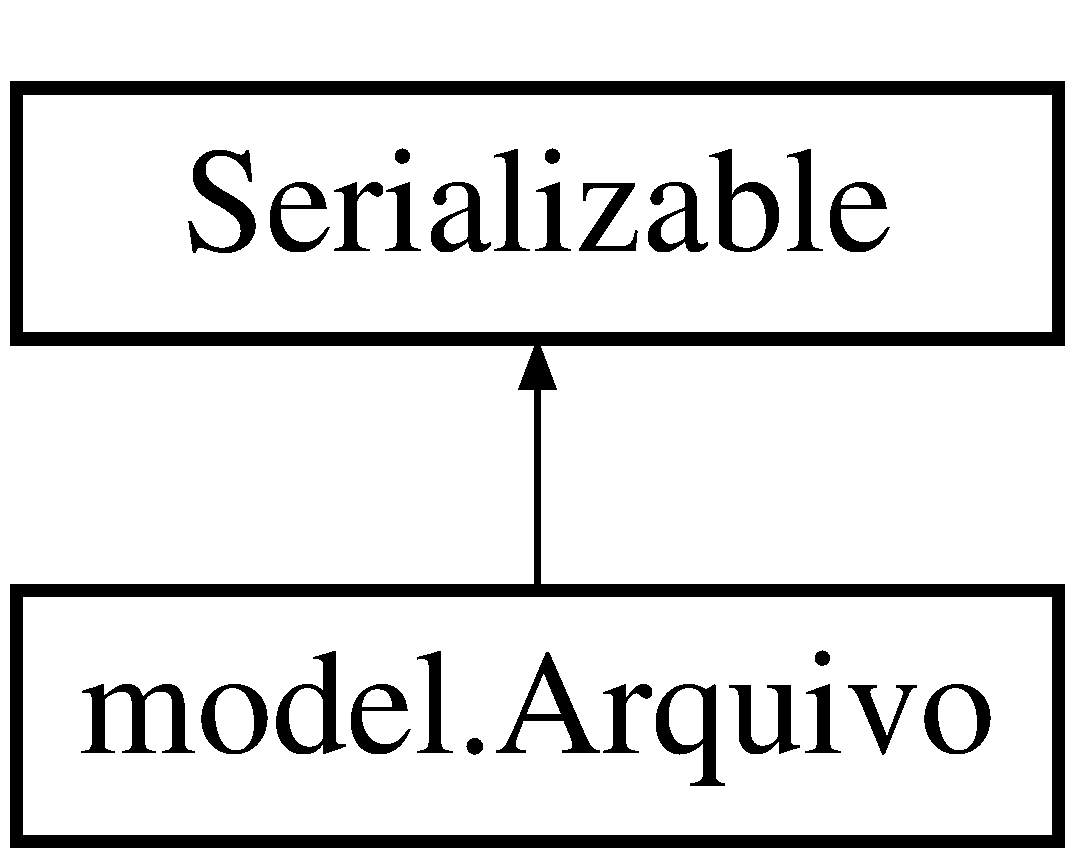
\includegraphics[height=2.000000cm]{classmodel_1_1_arquivo}
\end{center}
\end{figure}
\subsection*{Public Member Functions}
\begin{DoxyCompactItemize}
\item 
\hypertarget{classmodel_1_1_arquivo_a580693728bbdaa7906333c7e5de74190}{String {\bfseries to\+String} ()}\label{classmodel_1_1_arquivo_a580693728bbdaa7906333c7e5de74190}

\item 
\hypertarget{classmodel_1_1_arquivo_a7d033e942466ae8f3150d3ee26a4f3dc}{String {\bfseries get\+Nome} ()}\label{classmodel_1_1_arquivo_a7d033e942466ae8f3150d3ee26a4f3dc}

\item 
\hypertarget{classmodel_1_1_arquivo_aeb26ae518929ffb319923f2627f6efc6}{void {\bfseries set\+Nome} (String nome)}\label{classmodel_1_1_arquivo_aeb26ae518929ffb319923f2627f6efc6}

\item 
\hypertarget{classmodel_1_1_arquivo_ae952e3c2814c80659c9544172e8c7148}{float {\bfseries get\+Tamanho} ()}\label{classmodel_1_1_arquivo_ae952e3c2814c80659c9544172e8c7148}

\item 
\hypertarget{classmodel_1_1_arquivo_a72de705e73dc067a3224ab424d3d7c43}{void {\bfseries set\+Tamanho} (float tamanho)}\label{classmodel_1_1_arquivo_a72de705e73dc067a3224ab424d3d7c43}

\item 
\hypertarget{classmodel_1_1_arquivo_afb695a8c5c9351d13ecf8992a47c62fc}{Date {\bfseries get\+Data\+Criacao} ()}\label{classmodel_1_1_arquivo_afb695a8c5c9351d13ecf8992a47c62fc}

\item 
\hypertarget{classmodel_1_1_arquivo_a92ea42514e4c2fe33738a880ede6374e}{void {\bfseries set\+Data\+Criacao} (Date data\+Criacao)}\label{classmodel_1_1_arquivo_a92ea42514e4c2fe33738a880ede6374e}

\item 
\hypertarget{classmodel_1_1_arquivo_ac26be3a6809e5318d6f3ac6569ecaf46}{Date {\bfseries get\+Data\+Ultima\+Modificacao} ()}\label{classmodel_1_1_arquivo_ac26be3a6809e5318d6f3ac6569ecaf46}

\item 
\hypertarget{classmodel_1_1_arquivo_a9a1fcff51bb12d03d9e8acc97272c9fc}{void {\bfseries set\+Data\+Ultima\+Modificacao} (Date data\+Ultima\+Modificacao)}\label{classmodel_1_1_arquivo_a9a1fcff51bb12d03d9e8acc97272c9fc}

\item 
\hypertarget{classmodel_1_1_arquivo_a651184830b8c5ed0985167d3b77fc7ae}{String {\bfseries get\+Conteudo} ()}\label{classmodel_1_1_arquivo_a651184830b8c5ed0985167d3b77fc7ae}

\item 
\hypertarget{classmodel_1_1_arquivo_ab374f2d11f50ef294c12676fa560e673}{void {\bfseries set\+Conteudo} (String conteudo)}\label{classmodel_1_1_arquivo_ab374f2d11f50ef294c12676fa560e673}

\end{DoxyCompactItemize}


\subsection{Detailed Description}
Classe que implementa operações básicas sobre um arquivo

\begin{DoxyAuthor}{Author}
minoro 
\end{DoxyAuthor}


The documentation for this class was generated from the following file\+:\begin{DoxyCompactItemize}
\item 
src/model/Arquivo.\+java\end{DoxyCompactItemize}

\hypertarget{classcliente_1_1_cliente}{\section{cliente.\+Cliente Class Reference}
\label{classcliente_1_1_cliente}\index{cliente.\+Cliente@{cliente.\+Cliente}}
}
Inheritance diagram for cliente.\+Cliente\+:\begin{figure}[H]
\begin{center}
\leavevmode
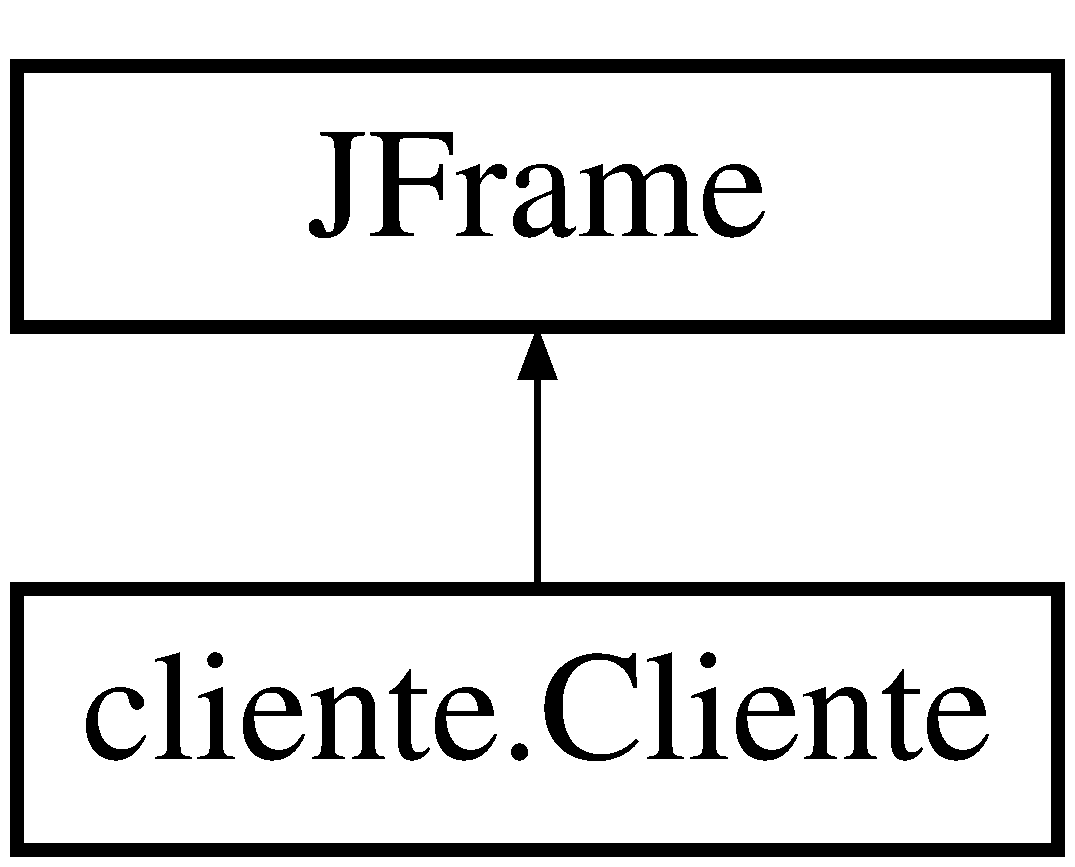
\includegraphics[height=2.000000cm]{classcliente_1_1_cliente}
\end{center}
\end{figure}
\subsection*{Public Member Functions}
\begin{DoxyCompactItemize}
\item 
\hyperlink{classcliente_1_1_cliente_a541ca7f31911cc2642cb081df9619931}{Cliente} ()
\end{DoxyCompactItemize}
\subsection*{Static Public Member Functions}
\begin{DoxyCompactItemize}
\item 
static void \hyperlink{classcliente_1_1_cliente_aa6bafb3ec499c400dd4b43e039d5131c}{main} (String args\mbox{[}$\,$\mbox{]})
\end{DoxyCompactItemize}


\subsection{Detailed Description}
\begin{DoxyAuthor}{Author}
Matheus 
\end{DoxyAuthor}


\subsection{Constructor \& Destructor Documentation}
\hypertarget{classcliente_1_1_cliente_a541ca7f31911cc2642cb081df9619931}{\index{cliente\+::\+Cliente@{cliente\+::\+Cliente}!Cliente@{Cliente}}
\index{Cliente@{Cliente}!cliente\+::\+Cliente@{cliente\+::\+Cliente}}
\subsubsection[{Cliente}]{\setlength{\rightskip}{0pt plus 5cm}cliente.\+Cliente.\+Cliente (
\begin{DoxyParamCaption}
{}
\end{DoxyParamCaption}
)}}\label{classcliente_1_1_cliente_a541ca7f31911cc2642cb081df9619931}
Creates new form \hyperlink{classcliente_1_1_cliente}{Cliente} 

\subsection{Member Function Documentation}
\hypertarget{classcliente_1_1_cliente_aa6bafb3ec499c400dd4b43e039d5131c}{\index{cliente\+::\+Cliente@{cliente\+::\+Cliente}!main@{main}}
\index{main@{main}!cliente\+::\+Cliente@{cliente\+::\+Cliente}}
\subsubsection[{main}]{\setlength{\rightskip}{0pt plus 5cm}static void cliente.\+Cliente.\+main (
\begin{DoxyParamCaption}
\item[{String}]{args\mbox{[}$\,$\mbox{]}}
\end{DoxyParamCaption}
)\hspace{0.3cm}{\ttfamily [static]}}}\label{classcliente_1_1_cliente_aa6bafb3ec499c400dd4b43e039d5131c}

\begin{DoxyParams}{Parameters}
{\em args} & the command line arguments \\
\hline
\end{DoxyParams}


The documentation for this class was generated from the following file\+:\begin{DoxyCompactItemize}
\item 
src/cliente/Cliente.\+java\end{DoxyCompactItemize}

\hypertarget{classforms_1_1_copiar_arquivo}{\section{forms.\+Copiar\+Arquivo Class Reference}
\label{classforms_1_1_copiar_arquivo}\index{forms.\+Copiar\+Arquivo@{forms.\+Copiar\+Arquivo}}
}
Inheritance diagram for forms.\+Copiar\+Arquivo\+:\begin{figure}[H]
\begin{center}
\leavevmode
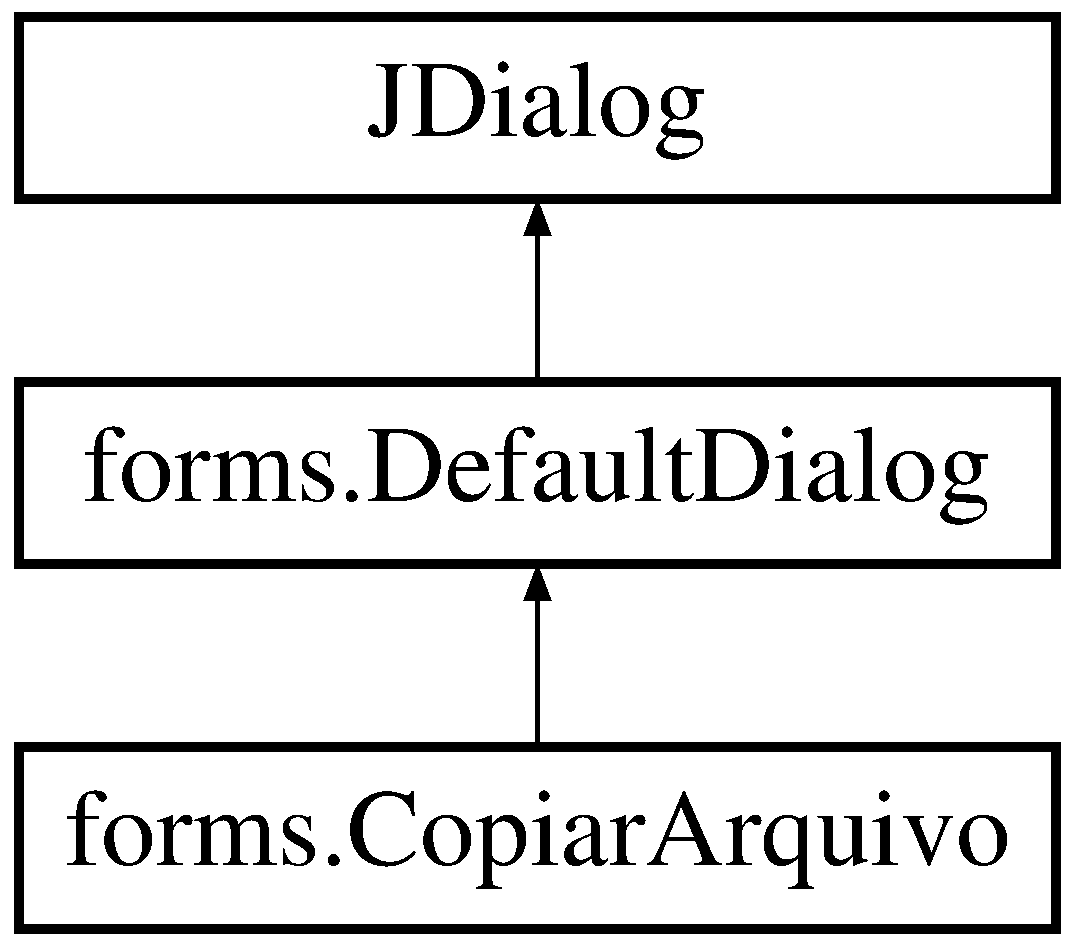
\includegraphics[height=3.000000cm]{classforms_1_1_copiar_arquivo}
\end{center}
\end{figure}
\subsection*{Public Member Functions}
\begin{DoxyCompactItemize}
\item 
\hyperlink{classforms_1_1_copiar_arquivo_a5f808b39debb3e730407ec79e279fe65}{Copiar\+Arquivo} (java.\+awt.\+Frame parent, boolean modal)
\end{DoxyCompactItemize}
\subsection*{Additional Inherited Members}


\subsection{Detailed Description}
\begin{DoxyAuthor}{Author}
Matheus 
\end{DoxyAuthor}


\subsection{Constructor \& Destructor Documentation}
\hypertarget{classforms_1_1_copiar_arquivo_a5f808b39debb3e730407ec79e279fe65}{\index{forms\+::\+Copiar\+Arquivo@{forms\+::\+Copiar\+Arquivo}!Copiar\+Arquivo@{Copiar\+Arquivo}}
\index{Copiar\+Arquivo@{Copiar\+Arquivo}!forms\+::\+Copiar\+Arquivo@{forms\+::\+Copiar\+Arquivo}}
\subsubsection[{Copiar\+Arquivo}]{\setlength{\rightskip}{0pt plus 5cm}forms.\+Copiar\+Arquivo.\+Copiar\+Arquivo (
\begin{DoxyParamCaption}
\item[{java.\+awt.\+Frame}]{parent, }
\item[{boolean}]{modal}
\end{DoxyParamCaption}
)}}\label{classforms_1_1_copiar_arquivo_a5f808b39debb3e730407ec79e279fe65}
Creates new form \hyperlink{classforms_1_1_copiar_arquivo}{Copiar\+Arquivo} 

The documentation for this class was generated from the following file\+:\begin{DoxyCompactItemize}
\item 
src/forms/Copiar\+Arquivo.\+java\end{DoxyCompactItemize}

\hypertarget{classforms_1_1_copiar_pasta}{\section{forms.\+Copiar\+Pasta Class Reference}
\label{classforms_1_1_copiar_pasta}\index{forms.\+Copiar\+Pasta@{forms.\+Copiar\+Pasta}}
}
Inheritance diagram for forms.\+Copiar\+Pasta\+:\begin{figure}[H]
\begin{center}
\leavevmode
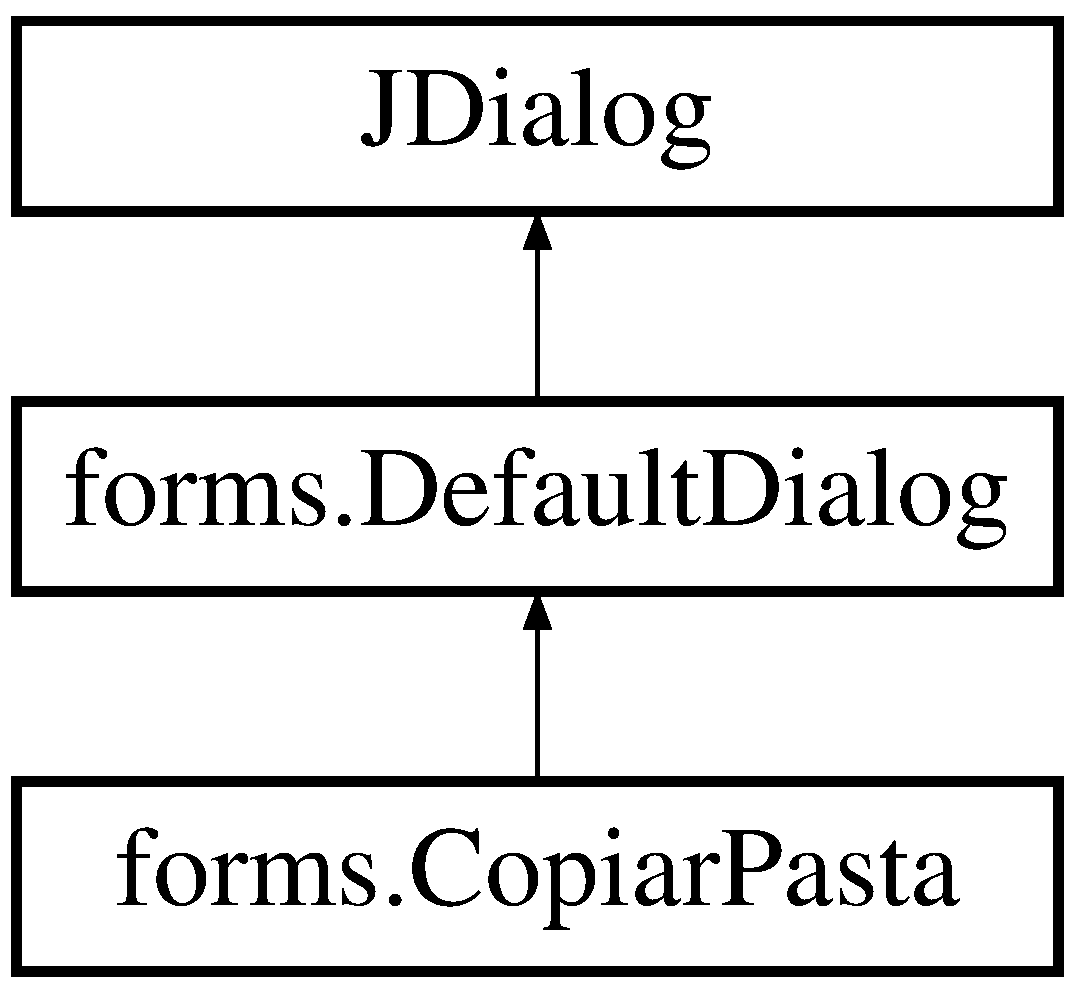
\includegraphics[height=3.000000cm]{classforms_1_1_copiar_pasta}
\end{center}
\end{figure}
\subsection*{Public Member Functions}
\begin{DoxyCompactItemize}
\item 
\hyperlink{classforms_1_1_copiar_pasta_af917360791ee284df8067818c1d522d5}{Copiar\+Pasta} (java.\+awt.\+Frame parent, boolean modal)
\end{DoxyCompactItemize}
\subsection*{Additional Inherited Members}


\subsection{Detailed Description}
\begin{DoxyAuthor}{Author}
Matheus 
\end{DoxyAuthor}


\subsection{Constructor \& Destructor Documentation}
\hypertarget{classforms_1_1_copiar_pasta_af917360791ee284df8067818c1d522d5}{\index{forms\+::\+Copiar\+Pasta@{forms\+::\+Copiar\+Pasta}!Copiar\+Pasta@{Copiar\+Pasta}}
\index{Copiar\+Pasta@{Copiar\+Pasta}!forms\+::\+Copiar\+Pasta@{forms\+::\+Copiar\+Pasta}}
\subsubsection[{Copiar\+Pasta}]{\setlength{\rightskip}{0pt plus 5cm}forms.\+Copiar\+Pasta.\+Copiar\+Pasta (
\begin{DoxyParamCaption}
\item[{java.\+awt.\+Frame}]{parent, }
\item[{boolean}]{modal}
\end{DoxyParamCaption}
)}}\label{classforms_1_1_copiar_pasta_af917360791ee284df8067818c1d522d5}
Creates new form \hyperlink{classforms_1_1_copiar_arquivo}{Copiar\+Arquivo} 

The documentation for this class was generated from the following file\+:\begin{DoxyCompactItemize}
\item 
src/forms/Copiar\+Pasta.\+java\end{DoxyCompactItemize}

\hypertarget{classforms_1_1_default_dialog}{\section{forms.\+Default\+Dialog Class Reference}
\label{classforms_1_1_default_dialog}\index{forms.\+Default\+Dialog@{forms.\+Default\+Dialog}}
}
Inheritance diagram for forms.\+Default\+Dialog\+:\begin{figure}[H]
\begin{center}
\leavevmode
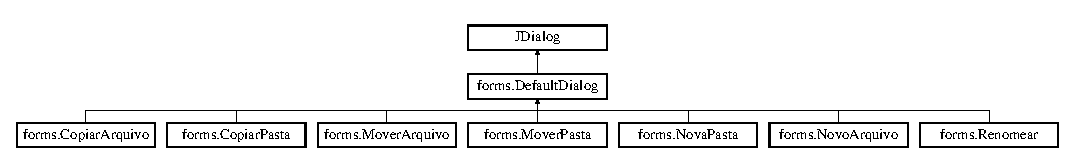
\includegraphics[height=1.751825cm]{classforms_1_1_default_dialog}
\end{center}
\end{figure}
\subsection*{Public Member Functions}
\begin{DoxyCompactItemize}
\item 
\hypertarget{classforms_1_1_default_dialog_a3af4fbc1582744720afe42567a65fb47}{{\bfseries Default\+Dialog} (java.\+awt.\+Frame parent, boolean modal)}\label{classforms_1_1_default_dialog_a3af4fbc1582744720afe42567a65fb47}

\end{DoxyCompactItemize}
\subsection*{Protected Member Functions}
\begin{DoxyCompactItemize}
\item 
void \hyperlink{classforms_1_1_default_dialog_a2d8fa1f5b3090c1fa2d15870a5159c77}{close} ()
\end{DoxyCompactItemize}


\subsection{Detailed Description}
\begin{DoxyAuthor}{Author}
Matheus 
\end{DoxyAuthor}


\subsection{Member Function Documentation}
\hypertarget{classforms_1_1_default_dialog_a2d8fa1f5b3090c1fa2d15870a5159c77}{\index{forms\+::\+Default\+Dialog@{forms\+::\+Default\+Dialog}!close@{close}}
\index{close@{close}!forms\+::\+Default\+Dialog@{forms\+::\+Default\+Dialog}}
\subsubsection[{close}]{\setlength{\rightskip}{0pt plus 5cm}void forms.\+Default\+Dialog.\+close (
\begin{DoxyParamCaption}
{}
\end{DoxyParamCaption}
)\hspace{0.3cm}{\ttfamily [protected]}}}\label{classforms_1_1_default_dialog_a2d8fa1f5b3090c1fa2d15870a5159c77}
Método personalizado para fechar a janela e atualizar a árvore de hierarquia automaticamente 

The documentation for this class was generated from the following file\+:\begin{DoxyCompactItemize}
\item 
src/forms/Default\+Dialog.\+java\end{DoxyCompactItemize}

\hypertarget{classservidor_1_1_gerenciador_arquivos}{\section{servidor.\+Gerenciador\+Arquivos Class Reference}
\label{classservidor_1_1_gerenciador_arquivos}\index{servidor.\+Gerenciador\+Arquivos@{servidor.\+Gerenciador\+Arquivos}}
}
\subsection*{Static Public Member Functions}
\begin{DoxyCompactItemize}
\item 
static String \hyperlink{classservidor_1_1_gerenciador_arquivos_a986e89c4c8c481eff09b7418c50ba69e}{criar\+Arquivo} (\hyperlink{classmodel_1_1_arquivo}{Arquivo} arquivo)
\item 
static boolean \hyperlink{classservidor_1_1_gerenciador_arquivos_a80c02193564d7e59ad81af60021a62ce}{apagar\+Arquivo} (String nome)
\item 
static boolean \hyperlink{classservidor_1_1_gerenciador_arquivos_a6252ba0a3ef659ea4d6082ea496be15a}{salvar\+Arquivo} (\hyperlink{classmodel_1_1_arquivo}{Arquivo} arquivo, String nome)
\item 
static \hyperlink{classmodel_1_1_arquivo}{Arquivo} \hyperlink{classservidor_1_1_gerenciador_arquivos_ac7505735f05bafbbd913db3ac3e858e8}{abrir\+Arquivo} (String nome)
\end{DoxyCompactItemize}


\subsection{Detailed Description}
Classe para manipular arquivos no servidor 

\subsection{Member Function Documentation}
\hypertarget{classservidor_1_1_gerenciador_arquivos_ac7505735f05bafbbd913db3ac3e858e8}{\index{servidor\+::\+Gerenciador\+Arquivos@{servidor\+::\+Gerenciador\+Arquivos}!abrir\+Arquivo@{abrir\+Arquivo}}
\index{abrir\+Arquivo@{abrir\+Arquivo}!servidor\+::\+Gerenciador\+Arquivos@{servidor\+::\+Gerenciador\+Arquivos}}
\subsubsection[{abrir\+Arquivo}]{\setlength{\rightskip}{0pt plus 5cm}static {\bf Arquivo} servidor.\+Gerenciador\+Arquivos.\+abrir\+Arquivo (
\begin{DoxyParamCaption}
\item[{String}]{nome}
\end{DoxyParamCaption}
)\hspace{0.3cm}{\ttfamily [static]}}}\label{classservidor_1_1_gerenciador_arquivos_ac7505735f05bafbbd913db3ac3e858e8}
Retorna um objeto Arquivo dado o nome aleatório de um arquivo persistido


\begin{DoxyParams}{Parameters}
{\em nome} & String -\/ nome aleatório do arquivo \\
\hline
\end{DoxyParams}
\begin{DoxyReturn}{Returns}
Arquivo -\/ retorna o objeto com seus atributos 
\end{DoxyReturn}
\hypertarget{classservidor_1_1_gerenciador_arquivos_a80c02193564d7e59ad81af60021a62ce}{\index{servidor\+::\+Gerenciador\+Arquivos@{servidor\+::\+Gerenciador\+Arquivos}!apagar\+Arquivo@{apagar\+Arquivo}}
\index{apagar\+Arquivo@{apagar\+Arquivo}!servidor\+::\+Gerenciador\+Arquivos@{servidor\+::\+Gerenciador\+Arquivos}}
\subsubsection[{apagar\+Arquivo}]{\setlength{\rightskip}{0pt plus 5cm}static boolean servidor.\+Gerenciador\+Arquivos.\+apagar\+Arquivo (
\begin{DoxyParamCaption}
\item[{String}]{nome}
\end{DoxyParamCaption}
)\hspace{0.3cm}{\ttfamily [static]}}}\label{classservidor_1_1_gerenciador_arquivos_a80c02193564d7e59ad81af60021a62ce}
Apaga um arquivo no disco do servidor


\begin{DoxyParams}{Parameters}
{\em nome} & String -\/ nome aleatório referente ao arquivo em disco \\
\hline
\end{DoxyParams}
\begin{DoxyReturn}{Returns}
boolean -\/ retorna true caso seja possível apagar o arquivo, falso caso não seja possível 
\end{DoxyReturn}
\hypertarget{classservidor_1_1_gerenciador_arquivos_a986e89c4c8c481eff09b7418c50ba69e}{\index{servidor\+::\+Gerenciador\+Arquivos@{servidor\+::\+Gerenciador\+Arquivos}!criar\+Arquivo@{criar\+Arquivo}}
\index{criar\+Arquivo@{criar\+Arquivo}!servidor\+::\+Gerenciador\+Arquivos@{servidor\+::\+Gerenciador\+Arquivos}}
\subsubsection[{criar\+Arquivo}]{\setlength{\rightskip}{0pt plus 5cm}static String servidor.\+Gerenciador\+Arquivos.\+criar\+Arquivo (
\begin{DoxyParamCaption}
\item[{{\bf Arquivo}}]{arquivo}
\end{DoxyParamCaption}
)\hspace{0.3cm}{\ttfamily [static]}}}\label{classservidor_1_1_gerenciador_arquivos_a986e89c4c8c481eff09b7418c50ba69e}
Cria um arquivo em disco caso não exista nenhum com o nome


\begin{DoxyParams}{Parameters}
{\em arquivo} & Arquivo -\/ Objeto do arquivo a ser salvo fisicamente \\
\hline
\end{DoxyParams}
\begin{DoxyReturn}{Returns}
String -\/ retorna um nome aleatório referente ao arquivo em disco caso seja possível criar o arquivo caso contrário retorna uma string vazia 
\end{DoxyReturn}
\hypertarget{classservidor_1_1_gerenciador_arquivos_a6252ba0a3ef659ea4d6082ea496be15a}{\index{servidor\+::\+Gerenciador\+Arquivos@{servidor\+::\+Gerenciador\+Arquivos}!salvar\+Arquivo@{salvar\+Arquivo}}
\index{salvar\+Arquivo@{salvar\+Arquivo}!servidor\+::\+Gerenciador\+Arquivos@{servidor\+::\+Gerenciador\+Arquivos}}
\subsubsection[{salvar\+Arquivo}]{\setlength{\rightskip}{0pt plus 5cm}static boolean servidor.\+Gerenciador\+Arquivos.\+salvar\+Arquivo (
\begin{DoxyParamCaption}
\item[{{\bf Arquivo}}]{arquivo, }
\item[{String}]{nome}
\end{DoxyParamCaption}
)\hspace{0.3cm}{\ttfamily [static]}}}\label{classservidor_1_1_gerenciador_arquivos_a6252ba0a3ef659ea4d6082ea496be15a}
Persiste o conteúdo de um objeto Arquivo em disco


\begin{DoxyParams}{Parameters}
{\em arquivo} & Arquivo -\/ objeto a ser persistido em disco \\
\hline
{\em nome} & String -\/ nome aleátorio gerado quando o arquivo é criado \\
\hline
\end{DoxyParams}
\begin{DoxyReturn}{Returns}
boolean -\/ retorna true caso seja possível salvar o arquivo ou false caso contrário 
\end{DoxyReturn}


The documentation for this class was generated from the following file\+:\begin{DoxyCompactItemize}
\item 
src/servidor/Gerenciador\+Arquivos.\+java\end{DoxyCompactItemize}

\hypertarget{classutils_1_1_g_m_a_s_editor}{\section{utils.\+G\+M\+A\+S\+Editor Class Reference}
\label{classutils_1_1_g_m_a_s_editor}\index{utils.\+G\+M\+A\+S\+Editor@{utils.\+G\+M\+A\+S\+Editor}}
}
Inheritance diagram for utils.\+G\+M\+A\+S\+Editor\+:\begin{figure}[H]
\begin{center}
\leavevmode
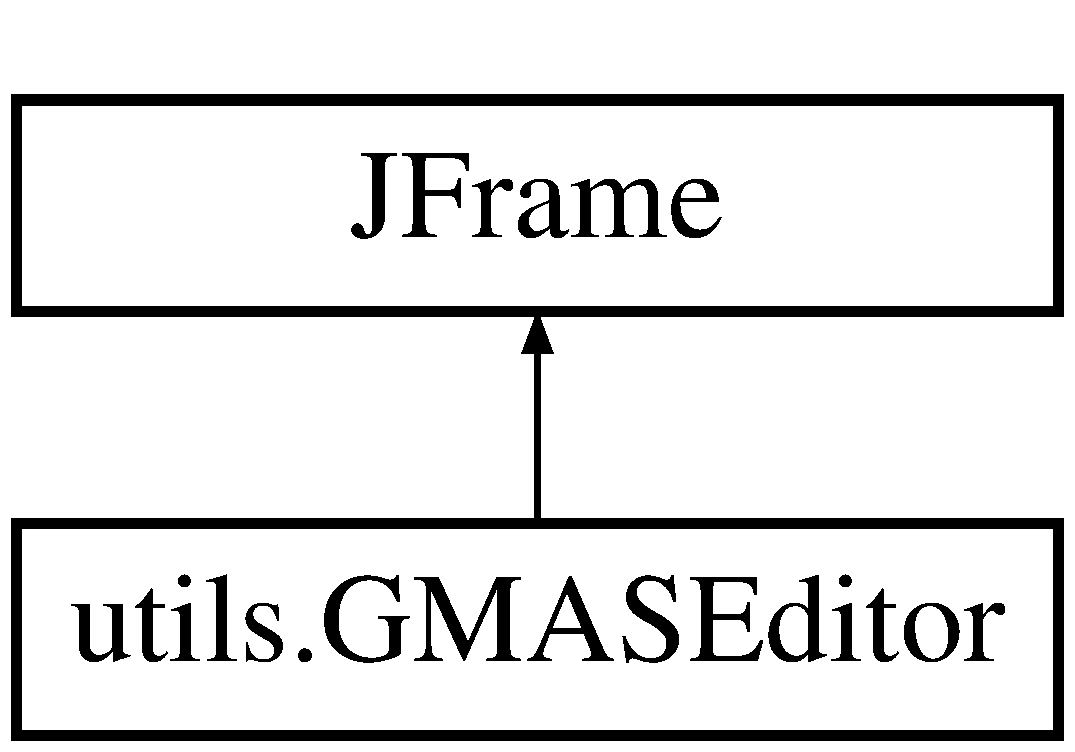
\includegraphics[height=2.000000cm]{classutils_1_1_g_m_a_s_editor}
\end{center}
\end{figure}
\subsection*{Public Member Functions}
\begin{DoxyCompactItemize}
\item 
\hypertarget{classutils_1_1_g_m_a_s_editor_a53dc984b80cc5707ae25170a7c52ed76}{{\bfseries G\+M\+A\+S\+Editor} (String conteudo, final String caminho)}\label{classutils_1_1_g_m_a_s_editor_a53dc984b80cc5707ae25170a7c52ed76}

\end{DoxyCompactItemize}


\subsection{Detailed Description}
\begin{DoxyAuthor}{Author}
mastelini 
\end{DoxyAuthor}


The documentation for this class was generated from the following file\+:\begin{DoxyCompactItemize}
\item 
src/utils/G\+M\+A\+S\+Editor.\+java\end{DoxyCompactItemize}

\hypertarget{classservidor_1_1_sistema_arquivo_1_1_heartbeat}{\section{servidor.\+Sistema\+Arquivo.\+Heartbeat Class Reference}
\label{classservidor_1_1_sistema_arquivo_1_1_heartbeat}\index{servidor.\+Sistema\+Arquivo.\+Heartbeat@{servidor.\+Sistema\+Arquivo.\+Heartbeat}}
}
Inheritance diagram for servidor.\+Sistema\+Arquivo.\+Heartbeat\+:\begin{figure}[H]
\begin{center}
\leavevmode
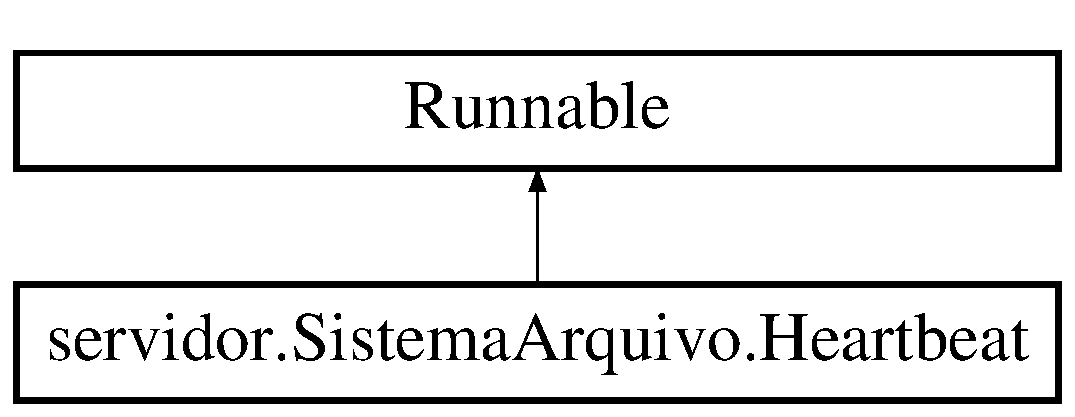
\includegraphics[height=2.000000cm]{classservidor_1_1_sistema_arquivo_1_1_heartbeat}
\end{center}
\end{figure}
\subsection*{Public Member Functions}
\begin{DoxyCompactItemize}
\item 
\hypertarget{classservidor_1_1_sistema_arquivo_1_1_heartbeat_ac20c759b24a8d0a0582b3f2f09844aac}{Inet\+Address {\bfseries get\+Ip} ()}\label{classservidor_1_1_sistema_arquivo_1_1_heartbeat_ac20c759b24a8d0a0582b3f2f09844aac}

\item 
\hypertarget{classservidor_1_1_sistema_arquivo_1_1_heartbeat_a42df0521bac88f23c79216595668b660}{int {\bfseries get\+Port} ()}\label{classservidor_1_1_sistema_arquivo_1_1_heartbeat_a42df0521bac88f23c79216595668b660}

\item 
\hypertarget{classservidor_1_1_sistema_arquivo_1_1_heartbeat_a8e9a74a8bdb6d218c2878b89e9f3096e}{{\bfseries Heartbeat} (Inet\+Address ip, int port)  throws I\+O\+Exception }\label{classservidor_1_1_sistema_arquivo_1_1_heartbeat_a8e9a74a8bdb6d218c2878b89e9f3096e}

\item 
\hypertarget{classservidor_1_1_sistema_arquivo_1_1_heartbeat_a00ddaefc53c383692a1b49c95471ba83}{void {\bfseries run} ()}\label{classservidor_1_1_sistema_arquivo_1_1_heartbeat_a00ddaefc53c383692a1b49c95471ba83}

\end{DoxyCompactItemize}


\subsection{Detailed Description}
Classe de \hyperlink{classservidor_1_1_sistema_arquivo_1_1_heartbeat}{Heartbeat}

\begin{DoxyAuthor}{Author}
Guilherme 
\end{DoxyAuthor}


The documentation for this class was generated from the following file\+:\begin{DoxyCompactItemize}
\item 
src/servidor/Sistema\+Arquivo.\+java\end{DoxyCompactItemize}

\hypertarget{classcliente_1_1_interface_usuario}{\section{cliente.\+Interface\+Usuario Class Reference}
\label{classcliente_1_1_interface_usuario}\index{cliente.\+Interface\+Usuario@{cliente.\+Interface\+Usuario}}
}
Inheritance diagram for cliente.\+Interface\+Usuario\+:\begin{figure}[H]
\begin{center}
\leavevmode
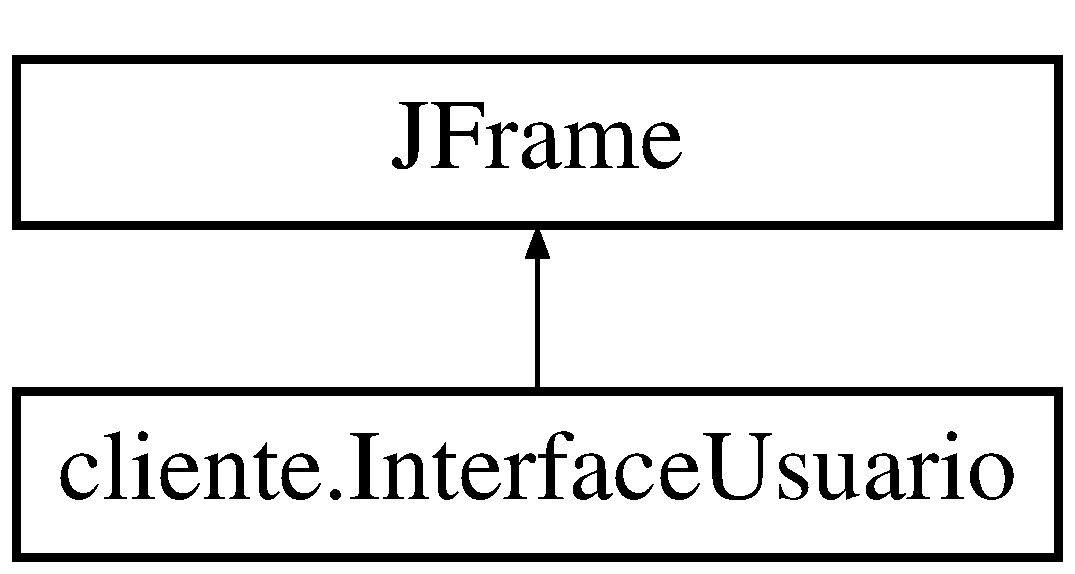
\includegraphics[height=2.000000cm]{classcliente_1_1_interface_usuario}
\end{center}
\end{figure}
\subsection*{Static Public Member Functions}
\begin{DoxyCompactItemize}
\item 
\hypertarget{classcliente_1_1_interface_usuario_a0bca7dbd254234fe3e611c10620a3b3e}{static void {\bfseries main} (String\mbox{[}$\,$\mbox{]} args)}\label{classcliente_1_1_interface_usuario_a0bca7dbd254234fe3e611c10620a3b3e}

\end{DoxyCompactItemize}
\subsection*{Static Public Attributes}
\begin{DoxyCompactItemize}
\item 
\hypertarget{classcliente_1_1_interface_usuario_ab1d1c90168b592e095f5863fd06df3ba}{static \hyperlink{classcliente_1_1_interface_usuario}{Interface\+Usuario} {\bfseries main}}\label{classcliente_1_1_interface_usuario_ab1d1c90168b592e095f5863fd06df3ba}

\item 
\hypertarget{classcliente_1_1_interface_usuario_a0eafac58bc9b15d9e0ba7f5e388f92f8}{static \hyperlink{classjtree_1_1_x_m_l_tree_panel}{X\+M\+L\+Tree\+Panel} {\bfseries panel}}\label{classcliente_1_1_interface_usuario_a0eafac58bc9b15d9e0ba7f5e388f92f8}

\end{DoxyCompactItemize}


The documentation for this class was generated from the following file\+:\begin{DoxyCompactItemize}
\item 
src/cliente/Interface\+Usuario.\+java\end{DoxyCompactItemize}

\hypertarget{classutils_1_1_manipulador_x_m_l}{\section{utils.\+Manipulador\+X\+M\+L Class Reference}
\label{classutils_1_1_manipulador_x_m_l}\index{utils.\+Manipulador\+X\+M\+L@{utils.\+Manipulador\+X\+M\+L}}
}
\subsection*{Public Member Functions}
\begin{DoxyCompactItemize}
\item 
\hypertarget{classutils_1_1_manipulador_x_m_l_a16a656452f4175f6429248f48e9e287f}{boolean {\bfseries existe\+Arquivo} (String caminho, Document xml)  throws X\+Path\+Expression\+Exception }\label{classutils_1_1_manipulador_x_m_l_a16a656452f4175f6429248f48e9e287f}

\item 
\hypertarget{classutils_1_1_manipulador_x_m_l_ad6c6eea5fc2af5a388ba9dc89c5ac58d}{boolean {\bfseries existe\+Pasta} (String caminho, Document xml)  throws X\+Path\+Expression\+Exception }\label{classutils_1_1_manipulador_x_m_l_ad6c6eea5fc2af5a388ba9dc89c5ac58d}

\item 
String \hyperlink{classutils_1_1_manipulador_x_m_l_abe6e542a9eaaae635a8a170b82440386}{montar\+Expressao\+Arquivo} (String caminho)
\item 
String \hyperlink{classutils_1_1_manipulador_x_m_l_a0c3294fa3f4ac2d40a6f544528acef53}{montar\+Expressao\+Pasta} (String caminho)
\item 
Node \hyperlink{classutils_1_1_manipulador_x_m_l_a0f077a38689257b4531ffc9068c9fe72}{pega\+Ultima\+Pasta} (String expressao, Document xml)  throws X\+Path\+Expression\+Exception 
\item 
Node \hyperlink{classutils_1_1_manipulador_x_m_l_a3722abbe1d67ed059d767625f145890c}{pega\+Ultimo\+Node} (String expressao, Document xml)  throws X\+Path\+Expression\+Exception 
\item 
boolean \hyperlink{classutils_1_1_manipulador_x_m_l_a8313756ee8243de3d89c2cb3ec3136ed}{salvar\+X\+M\+L} (Document xml, String nome\+Usuario)  throws Transformer\+Configuration\+Exception, Transformer\+Exception 
\item 
\hypertarget{classutils_1_1_manipulador_x_m_l_a508d4e44cb77093a9674a23aa47070f4}{String {\bfseries get\+Nome\+Arquivo\+Fisico} (String caminho, Document xml)  throws X\+Path\+Expression\+Exception }\label{classutils_1_1_manipulador_x_m_l_a508d4e44cb77093a9674a23aa47070f4}

\end{DoxyCompactItemize}
\subsection*{Static Public Member Functions}
\begin{DoxyCompactItemize}
\item 
\hypertarget{classutils_1_1_manipulador_x_m_l_ae359111e2e86584c59068ea934dfd90a}{static List$<$ String $>$ {\bfseries get\+Nomes\+Arquivos\+Fisicos} (Document xml)  throws X\+Path\+Expression\+Exception }\label{classutils_1_1_manipulador_x_m_l_ae359111e2e86584c59068ea934dfd90a}

\end{DoxyCompactItemize}


\subsection{Detailed Description}
Implementa operações simples para manipulação do X\+M\+L

\begin{DoxyAuthor}{Author}
minoro 
\end{DoxyAuthor}


\subsection{Member Function Documentation}
\hypertarget{classutils_1_1_manipulador_x_m_l_abe6e542a9eaaae635a8a170b82440386}{\index{utils\+::\+Manipulador\+X\+M\+L@{utils\+::\+Manipulador\+X\+M\+L}!montar\+Expressao\+Arquivo@{montar\+Expressao\+Arquivo}}
\index{montar\+Expressao\+Arquivo@{montar\+Expressao\+Arquivo}!utils\+::\+Manipulador\+X\+M\+L@{utils\+::\+Manipulador\+X\+M\+L}}
\subsubsection[{montar\+Expressao\+Arquivo}]{\setlength{\rightskip}{0pt plus 5cm}String utils.\+Manipulador\+X\+M\+L.\+montar\+Expressao\+Arquivo (
\begin{DoxyParamCaption}
\item[{String}]{caminho}
\end{DoxyParamCaption}
)}}\label{classutils_1_1_manipulador_x_m_l_abe6e542a9eaaae635a8a170b82440386}
Monta uma expressão para arquivo o X\+Path compilar


\begin{DoxyParams}{Parameters}
{\em caminho} & String -\/ caminho a ser gerado a expressao \\
\hline
\end{DoxyParams}
\begin{DoxyReturn}{Returns}
String -\/ retorna uma String representando a expressão do caminho do parâmetro 
\end{DoxyReturn}
\hypertarget{classutils_1_1_manipulador_x_m_l_a0c3294fa3f4ac2d40a6f544528acef53}{\index{utils\+::\+Manipulador\+X\+M\+L@{utils\+::\+Manipulador\+X\+M\+L}!montar\+Expressao\+Pasta@{montar\+Expressao\+Pasta}}
\index{montar\+Expressao\+Pasta@{montar\+Expressao\+Pasta}!utils\+::\+Manipulador\+X\+M\+L@{utils\+::\+Manipulador\+X\+M\+L}}
\subsubsection[{montar\+Expressao\+Pasta}]{\setlength{\rightskip}{0pt plus 5cm}String utils.\+Manipulador\+X\+M\+L.\+montar\+Expressao\+Pasta (
\begin{DoxyParamCaption}
\item[{String}]{caminho}
\end{DoxyParamCaption}
)}}\label{classutils_1_1_manipulador_x_m_l_a0c3294fa3f4ac2d40a6f544528acef53}
Monta uma expressão para pasta o X\+Path compilar


\begin{DoxyParams}{Parameters}
{\em caminho} & String -\/ caminho a ser gerado a expressao \\
\hline
\end{DoxyParams}
\begin{DoxyReturn}{Returns}
String -\/ retorna uma String representando a expressão do caminho do parâmetro 
\end{DoxyReturn}
\hypertarget{classutils_1_1_manipulador_x_m_l_a0f077a38689257b4531ffc9068c9fe72}{\index{utils\+::\+Manipulador\+X\+M\+L@{utils\+::\+Manipulador\+X\+M\+L}!pega\+Ultima\+Pasta@{pega\+Ultima\+Pasta}}
\index{pega\+Ultima\+Pasta@{pega\+Ultima\+Pasta}!utils\+::\+Manipulador\+X\+M\+L@{utils\+::\+Manipulador\+X\+M\+L}}
\subsubsection[{pega\+Ultima\+Pasta}]{\setlength{\rightskip}{0pt plus 5cm}Node utils.\+Manipulador\+X\+M\+L.\+pega\+Ultima\+Pasta (
\begin{DoxyParamCaption}
\item[{String}]{expressao, }
\item[{Document}]{xml}
\end{DoxyParamCaption}
) throws X\+Path\+Expression\+Exception}}\label{classutils_1_1_manipulador_x_m_l_a0f077a38689257b4531ffc9068c9fe72}
Dada uma expressão, retorna a última pasta dela. Utilizado para dar append\+Child.


\begin{DoxyParams}{Parameters}
{\em expressao} & String -\/ expressao X\+M\+L \\
\hline
{\em xml} & -\/ Document -\/ xml para ser pesquisado \\
\hline
\end{DoxyParams}
\begin{DoxyReturn}{Returns}
Node -\/ o nó da última pasta da expressão 
\end{DoxyReturn}

\begin{DoxyExceptions}{Exceptions}
{\em X\+Path\+Expression\+Exception} & \\
\hline
\end{DoxyExceptions}
\hypertarget{classutils_1_1_manipulador_x_m_l_a3722abbe1d67ed059d767625f145890c}{\index{utils\+::\+Manipulador\+X\+M\+L@{utils\+::\+Manipulador\+X\+M\+L}!pega\+Ultimo\+Node@{pega\+Ultimo\+Node}}
\index{pega\+Ultimo\+Node@{pega\+Ultimo\+Node}!utils\+::\+Manipulador\+X\+M\+L@{utils\+::\+Manipulador\+X\+M\+L}}
\subsubsection[{pega\+Ultimo\+Node}]{\setlength{\rightskip}{0pt plus 5cm}Node utils.\+Manipulador\+X\+M\+L.\+pega\+Ultimo\+Node (
\begin{DoxyParamCaption}
\item[{String}]{expressao, }
\item[{Document}]{xml}
\end{DoxyParamCaption}
) throws X\+Path\+Expression\+Exception}}\label{classutils_1_1_manipulador_x_m_l_a3722abbe1d67ed059d767625f145890c}

\begin{DoxyParams}{Parameters}
{\em expressao} & String -\/ expressao X\+M\+L \\
\hline
{\em xml} & -\/ Document -\/ xml a ser pesquisado \\
\hline
\end{DoxyParams}
\begin{DoxyReturn}{Returns}
Node -\/ o ultimo nó da expressão 
\end{DoxyReturn}

\begin{DoxyExceptions}{Exceptions}
{\em X\+Path\+Expression\+Exception} & \\
\hline
\end{DoxyExceptions}
\hypertarget{classutils_1_1_manipulador_x_m_l_a8313756ee8243de3d89c2cb3ec3136ed}{\index{utils\+::\+Manipulador\+X\+M\+L@{utils\+::\+Manipulador\+X\+M\+L}!salvar\+X\+M\+L@{salvar\+X\+M\+L}}
\index{salvar\+X\+M\+L@{salvar\+X\+M\+L}!utils\+::\+Manipulador\+X\+M\+L@{utils\+::\+Manipulador\+X\+M\+L}}
\subsubsection[{salvar\+X\+M\+L}]{\setlength{\rightskip}{0pt plus 5cm}boolean utils.\+Manipulador\+X\+M\+L.\+salvar\+X\+M\+L (
\begin{DoxyParamCaption}
\item[{Document}]{xml, }
\item[{String}]{nome\+Usuario}
\end{DoxyParamCaption}
) throws Transformer\+Configuration\+Exception, Transformer\+Exception}}\label{classutils_1_1_manipulador_x_m_l_a8313756ee8243de3d89c2cb3ec3136ed}
Salva o xml do parâmetro no arquivo físico


\begin{DoxyParams}{Parameters}
{\em nome\+Usuario} & String -\/ nome do usuário para ser salvo o arquivo X\+M\+L \\
\hline
{\em xml} & Document -\/ Objeto representando o arquivo xml \\
\hline
\end{DoxyParams}
\begin{DoxyReturn}{Returns}
boolean -\/ true caso salve o arquivo, false caso haja algum erro 
\end{DoxyReturn}

\begin{DoxyExceptions}{Exceptions}
{\em Transformer\+Configuration\+Exception} & \\
\hline
\end{DoxyExceptions}


The documentation for this class was generated from the following file\+:\begin{DoxyCompactItemize}
\item 
src/utils/Manipulador\+X\+M\+L.\+java\end{DoxyCompactItemize}

\hypertarget{classmiddleware_1_1_middleware}{\section{middleware.\+Middleware Class Reference}
\label{classmiddleware_1_1_middleware}\index{middleware.\+Middleware@{middleware.\+Middleware}}
}
\subsection*{Public Member Functions}
\begin{DoxyCompactItemize}
\item 
\hyperlink{classmiddleware_1_1_middleware_a2d7a099e82706c91ad5d5355c1959359}{Middleware} (String multicast\+Group, String nome\+Usuario, Boolean novo\+Usuario)  throws I\+O\+Exception, Unknown\+Host\+Exception, Remote\+Exception, X\+Path\+Expression\+Exception, Not\+Bound\+Exception 
\item 
String \hyperlink{classmiddleware_1_1_middleware_a3e838354f2f062385660c1c04681185e}{get\+U\+R\+L\+Servidor\+R\+M\+I} (int indice\+Servidor)
\item 
boolean \hyperlink{classmiddleware_1_1_middleware_a5f164a846ad486428469c7cdb79d985a}{renomear\+Arquivo} (String caminho, String nome\+\_\+digitado)  throws Remote\+Exception 
\item 
boolean \hyperlink{classmiddleware_1_1_middleware_a1ccaadf844107f004660ee209286dcd0}{criar\+Arquivo} (String caminho\+Selecionado, \hyperlink{classmodel_1_1_arquivo}{Arquivo} arquivo)  throws Remote\+Exception 
\item 
boolean \hyperlink{classmiddleware_1_1_middleware_a457ec4259716b0360c0ea38b5d30f86f}{criar\+Pasta} (String caminho\+Selecionado)  throws Remote\+Exception 
\item 
boolean \hyperlink{classmiddleware_1_1_middleware_a5656da24daf0e3e1ab472708a9ad3833}{copiar\+Arquivo} (String caminho\+Origem, String caminho\+Destino)  throws Remote\+Exception 
\item 
boolean \hyperlink{classmiddleware_1_1_middleware_ae299002971f601e9b4fcb7427c808f37}{copiar\+Pasta} (String caminho\+Origem, String caminho\+Destino)  throws Remote\+Exception 
\item 
void \hyperlink{classmiddleware_1_1_middleware_afac57d6d69b6fb3abf14bd8ec6d62737}{unlock} (String caminho)  throws Remote\+Exception 
\item 
boolean \hyperlink{classmiddleware_1_1_middleware_ae89884186ded30327bd4b02b781531b3}{mover\+Arquivo} (String caminho\+Origem, String caminho\+Destino)  throws Remote\+Exception 
\item 
boolean \hyperlink{classmiddleware_1_1_middleware_a258024d89a854e48edd71ce1dff7561f}{mover\+Pasta} (String caminho\+Origem, String caminho\+Destino)  throws Remote\+Exception 
\item 
boolean \hyperlink{classmiddleware_1_1_middleware_a91032b272523105aacae765b8d08d02b}{deletar\+Arquivo} (String caminho\+Origem)  throws Remote\+Exception 
\item 
boolean \hyperlink{classmiddleware_1_1_middleware_abd255ccfbaa4d1bf0344e4b4ddb79309}{deletar\+Pasta} (String caminho\+Origem)  throws Remote\+Exception 
\item 
boolean \hyperlink{classmiddleware_1_1_middleware_a3ce87937da7125149daf5b7838cbcdc7}{salvar\+Arquivo} (String caminho, String texto)  throws Remote\+Exception 
\item 
String \hyperlink{classmiddleware_1_1_middleware_a964d56555a150528a80f3ed4b892133f}{ler\+Arquivo} (String caminho)  throws Remote\+Exception 
\item 
Document \hyperlink{classmiddleware_1_1_middleware_a68f1d49902be780c30c4e44689f6b888}{pedir\+X\+M\+L} ()  throws Remote\+Exception 
\end{DoxyCompactItemize}
\subsection*{Public Attributes}
\begin{DoxyCompactItemize}
\item 
\hypertarget{classmiddleware_1_1_middleware_a6e83b6c280f87d8dc499b70297d76182}{List$<$ \hyperlink{interfaceservidor_1_1_sistema_arquivo_interface}{Sistema\+Arquivo\+Interface} $>$ {\bfseries servidores\+Remotos}}\label{classmiddleware_1_1_middleware_a6e83b6c280f87d8dc499b70297d76182}

\end{DoxyCompactItemize}


\subsection{Detailed Description}
Classe que realiza a comunicação entre a aplicação do cliente e os servidores de arquivo.

A comunicação é realizada através de chamadas R\+M\+I. Detecta falha de servidores e notifica um servidor desse fato, desencadeando um processo de recuperação de falhas 

\subsection{Constructor \& Destructor Documentation}
\hypertarget{classmiddleware_1_1_middleware_a2d7a099e82706c91ad5d5355c1959359}{\index{middleware\+::\+Middleware@{middleware\+::\+Middleware}!Middleware@{Middleware}}
\index{Middleware@{Middleware}!middleware\+::\+Middleware@{middleware\+::\+Middleware}}
\subsubsection[{Middleware}]{\setlength{\rightskip}{0pt plus 5cm}middleware.\+Middleware.\+Middleware (
\begin{DoxyParamCaption}
\item[{String}]{multicast\+Group, }
\item[{String}]{nome\+Usuario, }
\item[{Boolean}]{novo\+Usuario}
\end{DoxyParamCaption}
) throws I\+O\+Exception, Unknown\+Host\+Exception, Remote\+Exception, X\+Path\+Expression\+Exception, Not\+Bound\+Exception}}\label{classmiddleware_1_1_middleware_a2d7a099e82706c91ad5d5355c1959359}
Construtor da Classe de \hyperlink{classmiddleware_1_1_middleware}{Middleware}. A partir do endereço de um grupo Multicast passado por parametro envia uma solicitação para todos os servidores de arquivos remotos e, armazena na lista de servidores os dois primeiros que responderem a solicitação.


\begin{DoxyParams}{Parameters}
{\em multicast\+Group} & Endereço do grupo de multicast \\
\hline
{\em nome\+Usuario} & Nome do usuário \\
\hline
{\em novo\+Usuario} & Boolean que representa se é novo usuário ou não \\
\hline
\end{DoxyParams}

\begin{DoxyExceptions}{Exceptions}
{\em I\+O\+Exception} & \\
\hline
{\em java.\+net.\+Unknown\+Host\+Exception} & \\
\hline
{\em java.\+rmi.\+Remote\+Exception} & \\
\hline
{\em javax.\+xml.\+xpath.\+X\+Path\+Expression\+Exception} & \\
\hline
{\em java.\+rmi.\+Not\+Bound\+Exception} & \\
\hline
\end{DoxyExceptions}


\subsection{Member Function Documentation}
\hypertarget{classmiddleware_1_1_middleware_a5656da24daf0e3e1ab472708a9ad3833}{\index{middleware\+::\+Middleware@{middleware\+::\+Middleware}!copiar\+Arquivo@{copiar\+Arquivo}}
\index{copiar\+Arquivo@{copiar\+Arquivo}!middleware\+::\+Middleware@{middleware\+::\+Middleware}}
\subsubsection[{copiar\+Arquivo}]{\setlength{\rightskip}{0pt plus 5cm}boolean middleware.\+Middleware.\+copiar\+Arquivo (
\begin{DoxyParamCaption}
\item[{String}]{caminho\+Origem, }
\item[{String}]{caminho\+Destino}
\end{DoxyParamCaption}
) throws Remote\+Exception}}\label{classmiddleware_1_1_middleware_a5656da24daf0e3e1ab472708a9ad3833}
Realiza uma cópia de um arquivo no servidores


\begin{DoxyParams}{Parameters}
{\em caminho\+Origem} & Caminho de origem do arquivo \\
\hline
{\em caminho\+Destino} & Caminho de destino para a cópia \\
\hline
\end{DoxyParams}
\begin{DoxyReturn}{Returns}
true em caso de sucesso, senão false. 
\end{DoxyReturn}

\begin{DoxyExceptions}{Exceptions}
{\em Remote\+Exception} & \\
\hline
\end{DoxyExceptions}
\hypertarget{classmiddleware_1_1_middleware_ae299002971f601e9b4fcb7427c808f37}{\index{middleware\+::\+Middleware@{middleware\+::\+Middleware}!copiar\+Pasta@{copiar\+Pasta}}
\index{copiar\+Pasta@{copiar\+Pasta}!middleware\+::\+Middleware@{middleware\+::\+Middleware}}
\subsubsection[{copiar\+Pasta}]{\setlength{\rightskip}{0pt plus 5cm}boolean middleware.\+Middleware.\+copiar\+Pasta (
\begin{DoxyParamCaption}
\item[{String}]{caminho\+Origem, }
\item[{String}]{caminho\+Destino}
\end{DoxyParamCaption}
) throws Remote\+Exception}}\label{classmiddleware_1_1_middleware_ae299002971f601e9b4fcb7427c808f37}
Realiza a cópia de uma pasta nos servidores.


\begin{DoxyParams}{Parameters}
{\em caminho\+Origem} & Caminho de origem da pasta. \\
\hline
{\em caminho\+Destino} & Caminho de destino para a nova pasta. \\
\hline
\end{DoxyParams}
\begin{DoxyReturn}{Returns}
true em caso de sucesso, senão false. 
\end{DoxyReturn}

\begin{DoxyExceptions}{Exceptions}
{\em Remote\+Exception} & \\
\hline
\end{DoxyExceptions}
\hypertarget{classmiddleware_1_1_middleware_a1ccaadf844107f004660ee209286dcd0}{\index{middleware\+::\+Middleware@{middleware\+::\+Middleware}!criar\+Arquivo@{criar\+Arquivo}}
\index{criar\+Arquivo@{criar\+Arquivo}!middleware\+::\+Middleware@{middleware\+::\+Middleware}}
\subsubsection[{criar\+Arquivo}]{\setlength{\rightskip}{0pt plus 5cm}boolean middleware.\+Middleware.\+criar\+Arquivo (
\begin{DoxyParamCaption}
\item[{String}]{caminho\+Selecionado, }
\item[{{\bf Arquivo}}]{arquivo}
\end{DoxyParamCaption}
) throws Remote\+Exception}}\label{classmiddleware_1_1_middleware_a1ccaadf844107f004660ee209286dcd0}
Cria um novo arquivo nos servidores de armazenamento


\begin{DoxyParams}{Parameters}
{\em caminho\+Selecionado} & Caminho do arquivo \\
\hline
{\em arquivo} & Objeto representativo de arquivo (Model) \\
\hline
\end{DoxyParams}
\begin{DoxyReturn}{Returns}
True, se o arquivo foi criado com sucesso. False, em caso de falhas na criação.
\end{DoxyReturn}

\begin{DoxyExceptions}{Exceptions}
{\em Remote\+Exception} & \\
\hline
\end{DoxyExceptions}
\hypertarget{classmiddleware_1_1_middleware_a457ec4259716b0360c0ea38b5d30f86f}{\index{middleware\+::\+Middleware@{middleware\+::\+Middleware}!criar\+Pasta@{criar\+Pasta}}
\index{criar\+Pasta@{criar\+Pasta}!middleware\+::\+Middleware@{middleware\+::\+Middleware}}
\subsubsection[{criar\+Pasta}]{\setlength{\rightskip}{0pt plus 5cm}boolean middleware.\+Middleware.\+criar\+Pasta (
\begin{DoxyParamCaption}
\item[{String}]{caminho\+Selecionado}
\end{DoxyParamCaption}
) throws Remote\+Exception}}\label{classmiddleware_1_1_middleware_a457ec4259716b0360c0ea38b5d30f86f}
Cria uma nova pasta nos servidores de arquivos


\begin{DoxyParams}{Parameters}
{\em caminho\+Selecionado} & Caminho da nova pasta \\
\hline
\end{DoxyParams}
\begin{DoxyReturn}{Returns}
true em caso de sucesso, senão false. 
\end{DoxyReturn}

\begin{DoxyExceptions}{Exceptions}
{\em Remote\+Exception} & \\
\hline
\end{DoxyExceptions}
\hypertarget{classmiddleware_1_1_middleware_a91032b272523105aacae765b8d08d02b}{\index{middleware\+::\+Middleware@{middleware\+::\+Middleware}!deletar\+Arquivo@{deletar\+Arquivo}}
\index{deletar\+Arquivo@{deletar\+Arquivo}!middleware\+::\+Middleware@{middleware\+::\+Middleware}}
\subsubsection[{deletar\+Arquivo}]{\setlength{\rightskip}{0pt plus 5cm}boolean middleware.\+Middleware.\+deletar\+Arquivo (
\begin{DoxyParamCaption}
\item[{String}]{caminho\+Origem}
\end{DoxyParamCaption}
) throws Remote\+Exception}}\label{classmiddleware_1_1_middleware_a91032b272523105aacae765b8d08d02b}
Deleta um arquivo em todos os servidores relacionados a um cliente. 
\begin{DoxyParams}{Parameters}
{\em caminho\+Origem} & Caminho do arquivo. \\
\hline
\end{DoxyParams}
\begin{DoxyReturn}{Returns}
true em caso de sucesso, senão false. 
\end{DoxyReturn}

\begin{DoxyExceptions}{Exceptions}
{\em Remote\+Exception} & \\
\hline
\end{DoxyExceptions}
\hypertarget{classmiddleware_1_1_middleware_abd255ccfbaa4d1bf0344e4b4ddb79309}{\index{middleware\+::\+Middleware@{middleware\+::\+Middleware}!deletar\+Pasta@{deletar\+Pasta}}
\index{deletar\+Pasta@{deletar\+Pasta}!middleware\+::\+Middleware@{middleware\+::\+Middleware}}
\subsubsection[{deletar\+Pasta}]{\setlength{\rightskip}{0pt plus 5cm}boolean middleware.\+Middleware.\+deletar\+Pasta (
\begin{DoxyParamCaption}
\item[{String}]{caminho\+Origem}
\end{DoxyParamCaption}
) throws Remote\+Exception}}\label{classmiddleware_1_1_middleware_abd255ccfbaa4d1bf0344e4b4ddb79309}
Deleta uma pasta em todos os servidores de um determinado cliente. 
\begin{DoxyParams}{Parameters}
{\em caminho\+Origem} & Caminho do arquivo \\
\hline
\end{DoxyParams}
\begin{DoxyReturn}{Returns}
true em caso de sucesso, senão false. 
\end{DoxyReturn}

\begin{DoxyExceptions}{Exceptions}
{\em Remote\+Exception} & \\
\hline
\end{DoxyExceptions}
\hypertarget{classmiddleware_1_1_middleware_a3e838354f2f062385660c1c04681185e}{\index{middleware\+::\+Middleware@{middleware\+::\+Middleware}!get\+U\+R\+L\+Servidor\+R\+M\+I@{get\+U\+R\+L\+Servidor\+R\+M\+I}}
\index{get\+U\+R\+L\+Servidor\+R\+M\+I@{get\+U\+R\+L\+Servidor\+R\+M\+I}!middleware\+::\+Middleware@{middleware\+::\+Middleware}}
\subsubsection[{get\+U\+R\+L\+Servidor\+R\+M\+I}]{\setlength{\rightskip}{0pt plus 5cm}String middleware.\+Middleware.\+get\+U\+R\+L\+Servidor\+R\+M\+I (
\begin{DoxyParamCaption}
\item[{int}]{indice\+Servidor}
\end{DoxyParamCaption}
)}}\label{classmiddleware_1_1_middleware_a3e838354f2f062385660c1c04681185e}
Retorna a U\+R\+L R\+M\+I de um dos servidores relacionados ao cliente em questão.


\begin{DoxyParams}{Parameters}
{\em indice\+Servidor} & int -\/ indice do servidor para recuperação de I\+P \\
\hline
\end{DoxyParams}
\begin{DoxyReturn}{Returns}
U\+R\+L R\+M\+I do servidor de arquivo de índice \char`\"{}indice\+Servidor\char`\"{} 
\end{DoxyReturn}
\hypertarget{classmiddleware_1_1_middleware_a964d56555a150528a80f3ed4b892133f}{\index{middleware\+::\+Middleware@{middleware\+::\+Middleware}!ler\+Arquivo@{ler\+Arquivo}}
\index{ler\+Arquivo@{ler\+Arquivo}!middleware\+::\+Middleware@{middleware\+::\+Middleware}}
\subsubsection[{ler\+Arquivo}]{\setlength{\rightskip}{0pt plus 5cm}String middleware.\+Middleware.\+ler\+Arquivo (
\begin{DoxyParamCaption}
\item[{String}]{caminho}
\end{DoxyParamCaption}
) throws Remote\+Exception}}\label{classmiddleware_1_1_middleware_a964d56555a150528a80f3ed4b892133f}
Carrega o conteúdo de um arquivo. 
\begin{DoxyParams}{Parameters}
{\em caminho} & Caminho do arquivo selecionado. \\
\hline
\end{DoxyParams}
\begin{DoxyReturn}{Returns}
Retorna o conteúdo do arquivo selecionado na forma de uma string. 
\end{DoxyReturn}

\begin{DoxyExceptions}{Exceptions}
{\em Remote\+Exception} & \\
\hline
\end{DoxyExceptions}
\hypertarget{classmiddleware_1_1_middleware_ae89884186ded30327bd4b02b781531b3}{\index{middleware\+::\+Middleware@{middleware\+::\+Middleware}!mover\+Arquivo@{mover\+Arquivo}}
\index{mover\+Arquivo@{mover\+Arquivo}!middleware\+::\+Middleware@{middleware\+::\+Middleware}}
\subsubsection[{mover\+Arquivo}]{\setlength{\rightskip}{0pt plus 5cm}boolean middleware.\+Middleware.\+mover\+Arquivo (
\begin{DoxyParamCaption}
\item[{String}]{caminho\+Origem, }
\item[{String}]{caminho\+Destino}
\end{DoxyParamCaption}
) throws Remote\+Exception}}\label{classmiddleware_1_1_middleware_ae89884186ded30327bd4b02b781531b3}
Move um arquivo em todos os servidores do cliente em questão. 
\begin{DoxyParams}{Parameters}
{\em caminho\+Origem} & Caminho de origem do arquivo a ser movido. \\
\hline
{\em caminho\+Destino} & Caminho de destino para o arquivo. \\
\hline
\end{DoxyParams}
\begin{DoxyReturn}{Returns}
true em caso de sucesso, senão false. 
\end{DoxyReturn}

\begin{DoxyExceptions}{Exceptions}
{\em Remote\+Exception} & \\
\hline
\end{DoxyExceptions}
\hypertarget{classmiddleware_1_1_middleware_a258024d89a854e48edd71ce1dff7561f}{\index{middleware\+::\+Middleware@{middleware\+::\+Middleware}!mover\+Pasta@{mover\+Pasta}}
\index{mover\+Pasta@{mover\+Pasta}!middleware\+::\+Middleware@{middleware\+::\+Middleware}}
\subsubsection[{mover\+Pasta}]{\setlength{\rightskip}{0pt plus 5cm}boolean middleware.\+Middleware.\+mover\+Pasta (
\begin{DoxyParamCaption}
\item[{String}]{caminho\+Origem, }
\item[{String}]{caminho\+Destino}
\end{DoxyParamCaption}
) throws Remote\+Exception}}\label{classmiddleware_1_1_middleware_a258024d89a854e48edd71ce1dff7561f}
Move uma pasta em todos os servidores de arquivo de um determinado cliente. 
\begin{DoxyParams}{Parameters}
{\em caminho\+Origem} & Caminho de origem do arquivo. \\
\hline
{\em caminho\+Destino} & Caminho de destino para mover a pasta. \\
\hline
\end{DoxyParams}
\begin{DoxyReturn}{Returns}
true em caso de sucesso, senão false. 
\end{DoxyReturn}

\begin{DoxyExceptions}{Exceptions}
{\em Remote\+Exception} & \\
\hline
\end{DoxyExceptions}
\hypertarget{classmiddleware_1_1_middleware_a68f1d49902be780c30c4e44689f6b888}{\index{middleware\+::\+Middleware@{middleware\+::\+Middleware}!pedir\+X\+M\+L@{pedir\+X\+M\+L}}
\index{pedir\+X\+M\+L@{pedir\+X\+M\+L}!middleware\+::\+Middleware@{middleware\+::\+Middleware}}
\subsubsection[{pedir\+X\+M\+L}]{\setlength{\rightskip}{0pt plus 5cm}Document middleware.\+Middleware.\+pedir\+X\+M\+L (
\begin{DoxyParamCaption}
{}
\end{DoxyParamCaption}
) throws Remote\+Exception}}\label{classmiddleware_1_1_middleware_a68f1d49902be780c30c4e44689f6b888}
Requisita o xml para os servidores, representado na forma de um objeto. \begin{DoxyReturn}{Returns}
Retorna um objeto do tipo Document, representando o arquivo xml. 
\end{DoxyReturn}

\begin{DoxyExceptions}{Exceptions}
{\em Remote\+Exception} & \\
\hline
\end{DoxyExceptions}
\hypertarget{classmiddleware_1_1_middleware_a5f164a846ad486428469c7cdb79d985a}{\index{middleware\+::\+Middleware@{middleware\+::\+Middleware}!renomear\+Arquivo@{renomear\+Arquivo}}
\index{renomear\+Arquivo@{renomear\+Arquivo}!middleware\+::\+Middleware@{middleware\+::\+Middleware}}
\subsubsection[{renomear\+Arquivo}]{\setlength{\rightskip}{0pt plus 5cm}boolean middleware.\+Middleware.\+renomear\+Arquivo (
\begin{DoxyParamCaption}
\item[{String}]{caminho, }
\item[{String}]{nome\+\_\+digitado}
\end{DoxyParamCaption}
) throws Remote\+Exception}}\label{classmiddleware_1_1_middleware_a5f164a846ad486428469c7cdb79d985a}
Método intermediário entre a aplicação cliente e as chamadas R\+M\+I para os servidores.

Renomeia um arquivo em todos servidores que o armazenam. 
\begin{DoxyParams}{Parameters}
{\em caminho} & Caminho teórico do arquivo armazenado. \\
\hline
{\em nome\+\_\+digitado} & Novo nome para renomeação. \\
\hline
\end{DoxyParams}
\begin{DoxyReturn}{Returns}
True, se o arquivo foi renomeado com sucesso. False, em caso de falhas na renomeação. 
\end{DoxyReturn}

\begin{DoxyExceptions}{Exceptions}
{\em Remote\+Exception} & \\
\hline
\end{DoxyExceptions}
\hypertarget{classmiddleware_1_1_middleware_a3ce87937da7125149daf5b7838cbcdc7}{\index{middleware\+::\+Middleware@{middleware\+::\+Middleware}!salvar\+Arquivo@{salvar\+Arquivo}}
\index{salvar\+Arquivo@{salvar\+Arquivo}!middleware\+::\+Middleware@{middleware\+::\+Middleware}}
\subsubsection[{salvar\+Arquivo}]{\setlength{\rightskip}{0pt plus 5cm}boolean middleware.\+Middleware.\+salvar\+Arquivo (
\begin{DoxyParamCaption}
\item[{String}]{caminho, }
\item[{String}]{texto}
\end{DoxyParamCaption}
) throws Remote\+Exception}}\label{classmiddleware_1_1_middleware_a3ce87937da7125149daf5b7838cbcdc7}
Salva as alterações feitas em um arquivo em todos os servidores que o armazenam 
\begin{DoxyParams}{Parameters}
{\em caminho} & Caminho do arquivo. \\
\hline
{\em texto} & Conteúdo do arquivo. \\
\hline
\end{DoxyParams}
\begin{DoxyReturn}{Returns}
true em caso de sucesso, senão false. 
\end{DoxyReturn}

\begin{DoxyExceptions}{Exceptions}
{\em Remote\+Exception} & \\
\hline
\end{DoxyExceptions}
\hypertarget{classmiddleware_1_1_middleware_afac57d6d69b6fb3abf14bd8ec6d62737}{\index{middleware\+::\+Middleware@{middleware\+::\+Middleware}!unlock@{unlock}}
\index{unlock@{unlock}!middleware\+::\+Middleware@{middleware\+::\+Middleware}}
\subsubsection[{unlock}]{\setlength{\rightskip}{0pt plus 5cm}void middleware.\+Middleware.\+unlock (
\begin{DoxyParamCaption}
\item[{String}]{caminho}
\end{DoxyParamCaption}
) throws Remote\+Exception}}\label{classmiddleware_1_1_middleware_afac57d6d69b6fb3abf14bd8ec6d62737}
Desbloqueia um arquivo para edição por outras conexões de um mesmo usuário (conexões simultâneas). 
\begin{DoxyParams}{Parameters}
{\em caminho} & Caminho do arquivo para desbloqueio. \\
\hline
\end{DoxyParams}

\begin{DoxyExceptions}{Exceptions}
{\em Remote\+Exception} & \\
\hline
\end{DoxyExceptions}


The documentation for this class was generated from the following file\+:\begin{DoxyCompactItemize}
\item 
src/middleware/Middleware.\+java\end{DoxyCompactItemize}

\hypertarget{classforms_1_1_mover_arquivo}{\section{forms.\+Mover\+Arquivo Class Reference}
\label{classforms_1_1_mover_arquivo}\index{forms.\+Mover\+Arquivo@{forms.\+Mover\+Arquivo}}
}
Inheritance diagram for forms.\+Mover\+Arquivo\+:\begin{figure}[H]
\begin{center}
\leavevmode
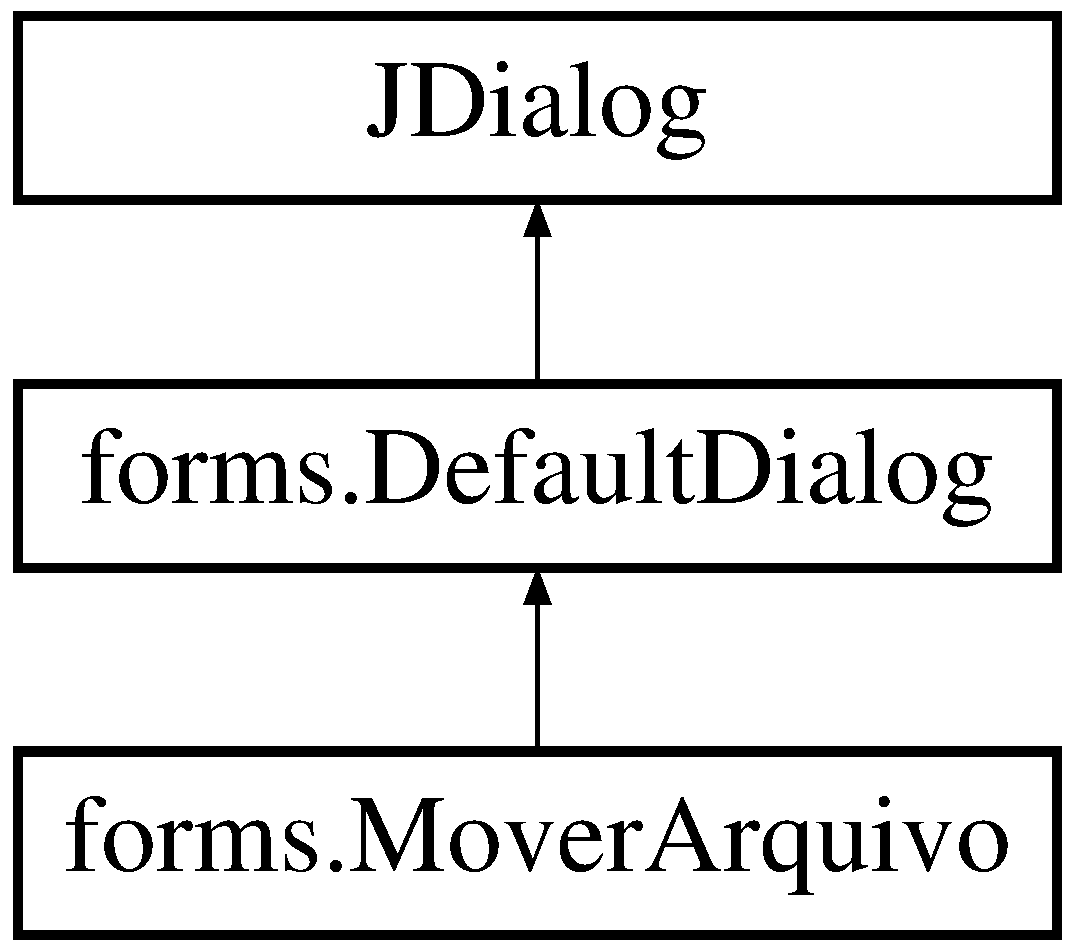
\includegraphics[height=3.000000cm]{classforms_1_1_mover_arquivo}
\end{center}
\end{figure}
\subsection*{Public Member Functions}
\begin{DoxyCompactItemize}
\item 
\hyperlink{classforms_1_1_mover_arquivo_a30ccd74777860ef511bbfe56afff1a7a}{Mover\+Arquivo} (java.\+awt.\+Frame parent, boolean modal)
\end{DoxyCompactItemize}
\subsection*{Additional Inherited Members}


\subsection{Detailed Description}
\begin{DoxyAuthor}{Author}
Matheus 
\end{DoxyAuthor}


\subsection{Constructor \& Destructor Documentation}
\hypertarget{classforms_1_1_mover_arquivo_a30ccd74777860ef511bbfe56afff1a7a}{\index{forms\+::\+Mover\+Arquivo@{forms\+::\+Mover\+Arquivo}!Mover\+Arquivo@{Mover\+Arquivo}}
\index{Mover\+Arquivo@{Mover\+Arquivo}!forms\+::\+Mover\+Arquivo@{forms\+::\+Mover\+Arquivo}}
\subsubsection[{Mover\+Arquivo}]{\setlength{\rightskip}{0pt plus 5cm}forms.\+Mover\+Arquivo.\+Mover\+Arquivo (
\begin{DoxyParamCaption}
\item[{java.\+awt.\+Frame}]{parent, }
\item[{boolean}]{modal}
\end{DoxyParamCaption}
)}}\label{classforms_1_1_mover_arquivo_a30ccd74777860ef511bbfe56afff1a7a}
Creates new form \hyperlink{classforms_1_1_mover_arquivo}{Mover\+Arquivo} 

The documentation for this class was generated from the following file\+:\begin{DoxyCompactItemize}
\item 
src/forms/Mover\+Arquivo.\+java\end{DoxyCompactItemize}

\hypertarget{classforms_1_1_mover_pasta}{\section{forms.\+Mover\+Pasta Class Reference}
\label{classforms_1_1_mover_pasta}\index{forms.\+Mover\+Pasta@{forms.\+Mover\+Pasta}}
}
Inheritance diagram for forms.\+Mover\+Pasta\+:\begin{figure}[H]
\begin{center}
\leavevmode
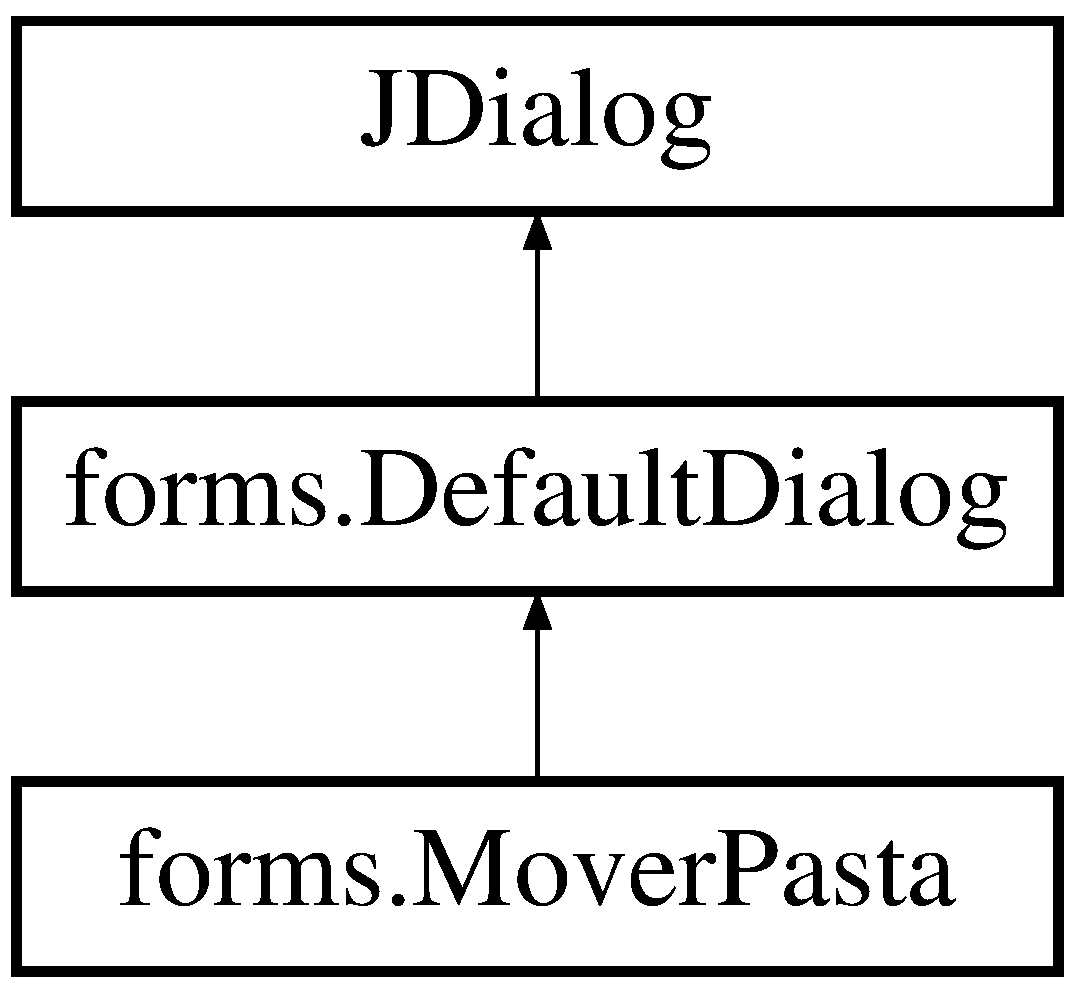
\includegraphics[height=3.000000cm]{classforms_1_1_mover_pasta}
\end{center}
\end{figure}
\subsection*{Public Member Functions}
\begin{DoxyCompactItemize}
\item 
\hyperlink{classforms_1_1_mover_pasta_a6dfd2e3acc4afc4be7313af1dd32355a}{Mover\+Pasta} (java.\+awt.\+Frame parent, boolean modal)
\end{DoxyCompactItemize}
\subsection*{Additional Inherited Members}


\subsection{Detailed Description}
\begin{DoxyAuthor}{Author}
Matheus 
\end{DoxyAuthor}


\subsection{Constructor \& Destructor Documentation}
\hypertarget{classforms_1_1_mover_pasta_a6dfd2e3acc4afc4be7313af1dd32355a}{\index{forms\+::\+Mover\+Pasta@{forms\+::\+Mover\+Pasta}!Mover\+Pasta@{Mover\+Pasta}}
\index{Mover\+Pasta@{Mover\+Pasta}!forms\+::\+Mover\+Pasta@{forms\+::\+Mover\+Pasta}}
\subsubsection[{Mover\+Pasta}]{\setlength{\rightskip}{0pt plus 5cm}forms.\+Mover\+Pasta.\+Mover\+Pasta (
\begin{DoxyParamCaption}
\item[{java.\+awt.\+Frame}]{parent, }
\item[{boolean}]{modal}
\end{DoxyParamCaption}
)}}\label{classforms_1_1_mover_pasta_a6dfd2e3acc4afc4be7313af1dd32355a}
Creates new form \hyperlink{classforms_1_1_mover_arquivo}{Mover\+Arquivo} 

The documentation for this class was generated from the following file\+:\begin{DoxyCompactItemize}
\item 
src/forms/Mover\+Pasta.\+java\end{DoxyCompactItemize}

\hypertarget{classforms_1_1_nova_pasta}{\section{forms.\+Nova\+Pasta Class Reference}
\label{classforms_1_1_nova_pasta}\index{forms.\+Nova\+Pasta@{forms.\+Nova\+Pasta}}
}
Inheritance diagram for forms.\+Nova\+Pasta\+:\begin{figure}[H]
\begin{center}
\leavevmode
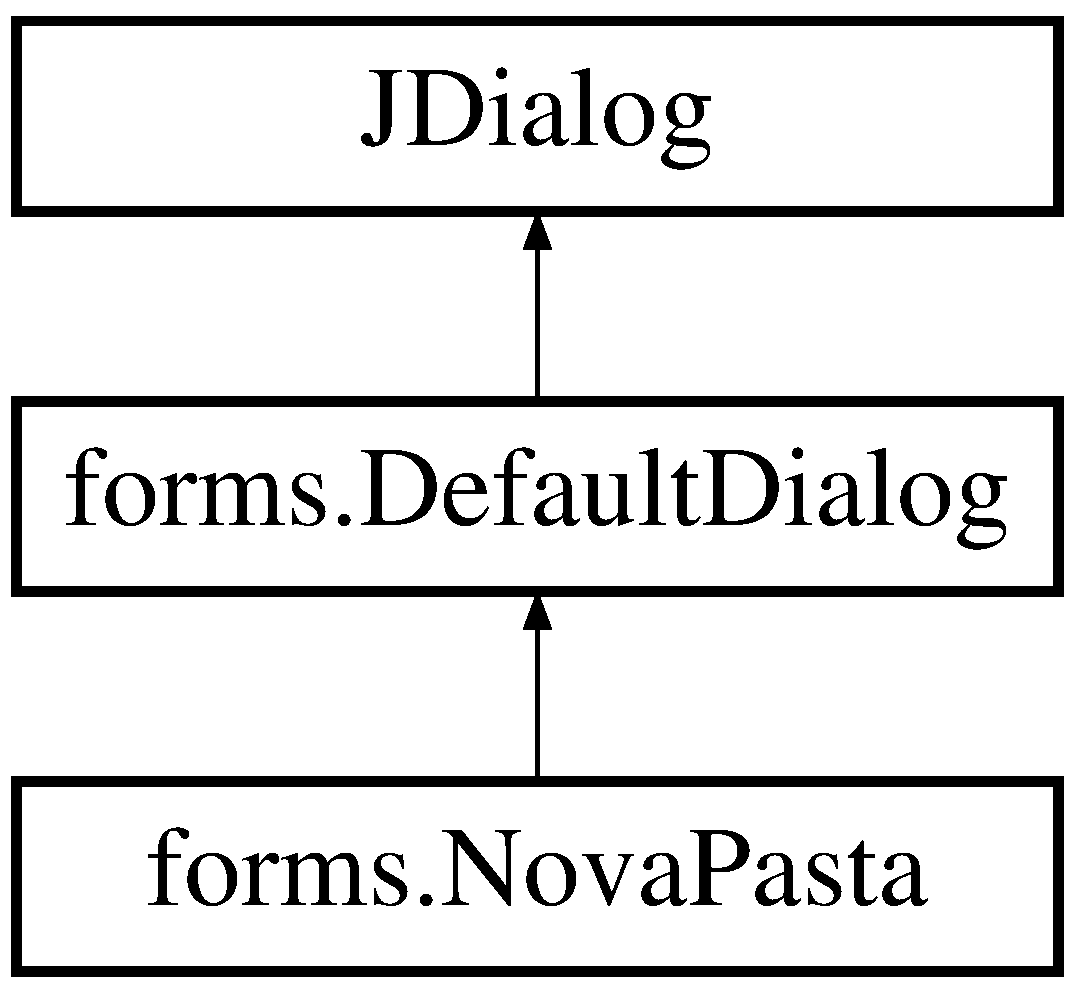
\includegraphics[height=3.000000cm]{classforms_1_1_nova_pasta}
\end{center}
\end{figure}
\subsection*{Public Member Functions}
\begin{DoxyCompactItemize}
\item 
\hyperlink{classforms_1_1_nova_pasta_a5d37e732079eb24bdb8a3c5ee30a8484}{Nova\+Pasta} (java.\+awt.\+Frame parent, boolean modal)
\end{DoxyCompactItemize}
\subsection*{Static Public Member Functions}
\begin{DoxyCompactItemize}
\item 
static void \hyperlink{classforms_1_1_nova_pasta_a1f36e0af1fca5787a4bfb508be6e60ee}{main} (String args\mbox{[}$\,$\mbox{]})
\end{DoxyCompactItemize}
\subsection*{Additional Inherited Members}


\subsection{Detailed Description}
\begin{DoxyAuthor}{Author}
Matheus 
\end{DoxyAuthor}


\subsection{Constructor \& Destructor Documentation}
\hypertarget{classforms_1_1_nova_pasta_a5d37e732079eb24bdb8a3c5ee30a8484}{\index{forms\+::\+Nova\+Pasta@{forms\+::\+Nova\+Pasta}!Nova\+Pasta@{Nova\+Pasta}}
\index{Nova\+Pasta@{Nova\+Pasta}!forms\+::\+Nova\+Pasta@{forms\+::\+Nova\+Pasta}}
\subsubsection[{Nova\+Pasta}]{\setlength{\rightskip}{0pt plus 5cm}forms.\+Nova\+Pasta.\+Nova\+Pasta (
\begin{DoxyParamCaption}
\item[{java.\+awt.\+Frame}]{parent, }
\item[{boolean}]{modal}
\end{DoxyParamCaption}
)}}\label{classforms_1_1_nova_pasta_a5d37e732079eb24bdb8a3c5ee30a8484}
Creates new form \hyperlink{classforms_1_1_nova_pasta}{Nova\+Pasta} 

\subsection{Member Function Documentation}
\hypertarget{classforms_1_1_nova_pasta_a1f36e0af1fca5787a4bfb508be6e60ee}{\index{forms\+::\+Nova\+Pasta@{forms\+::\+Nova\+Pasta}!main@{main}}
\index{main@{main}!forms\+::\+Nova\+Pasta@{forms\+::\+Nova\+Pasta}}
\subsubsection[{main}]{\setlength{\rightskip}{0pt plus 5cm}static void forms.\+Nova\+Pasta.\+main (
\begin{DoxyParamCaption}
\item[{String}]{args\mbox{[}$\,$\mbox{]}}
\end{DoxyParamCaption}
)\hspace{0.3cm}{\ttfamily [static]}}}\label{classforms_1_1_nova_pasta_a1f36e0af1fca5787a4bfb508be6e60ee}

\begin{DoxyParams}{Parameters}
{\em args} & the command line arguments \\
\hline
\end{DoxyParams}


The documentation for this class was generated from the following file\+:\begin{DoxyCompactItemize}
\item 
src/forms/Nova\+Pasta.\+java\end{DoxyCompactItemize}

\hypertarget{classforms_1_1_novo_arquivo}{\section{forms.\+Novo\+Arquivo Class Reference}
\label{classforms_1_1_novo_arquivo}\index{forms.\+Novo\+Arquivo@{forms.\+Novo\+Arquivo}}
}
Inheritance diagram for forms.\+Novo\+Arquivo\+:\begin{figure}[H]
\begin{center}
\leavevmode
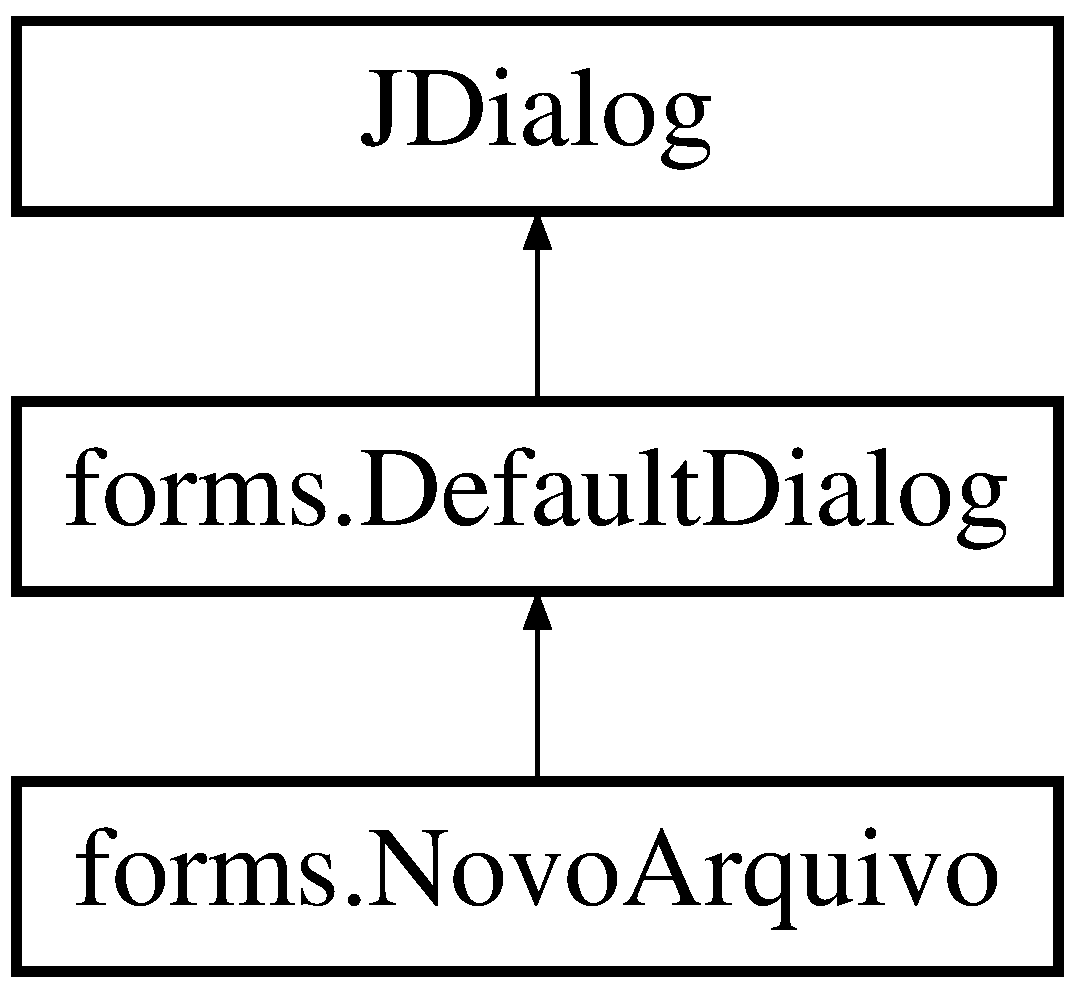
\includegraphics[height=3.000000cm]{classforms_1_1_novo_arquivo}
\end{center}
\end{figure}
\subsection*{Public Member Functions}
\begin{DoxyCompactItemize}
\item 
\hyperlink{classforms_1_1_novo_arquivo_a8b888c0fd02136097353bb8030dfa283}{Novo\+Arquivo} (java.\+awt.\+Frame parent, boolean modal)
\end{DoxyCompactItemize}
\subsection*{Static Public Member Functions}
\begin{DoxyCompactItemize}
\item 
static void \hyperlink{classforms_1_1_novo_arquivo_a68982a9f6a69dc98ef6062e4b45f2e12}{main} (String args\mbox{[}$\,$\mbox{]})
\end{DoxyCompactItemize}
\subsection*{Additional Inherited Members}


\subsection{Detailed Description}
\begin{DoxyAuthor}{Author}
Matheus 
\end{DoxyAuthor}


\subsection{Constructor \& Destructor Documentation}
\hypertarget{classforms_1_1_novo_arquivo_a8b888c0fd02136097353bb8030dfa283}{\index{forms\+::\+Novo\+Arquivo@{forms\+::\+Novo\+Arquivo}!Novo\+Arquivo@{Novo\+Arquivo}}
\index{Novo\+Arquivo@{Novo\+Arquivo}!forms\+::\+Novo\+Arquivo@{forms\+::\+Novo\+Arquivo}}
\subsubsection[{Novo\+Arquivo}]{\setlength{\rightskip}{0pt plus 5cm}forms.\+Novo\+Arquivo.\+Novo\+Arquivo (
\begin{DoxyParamCaption}
\item[{java.\+awt.\+Frame}]{parent, }
\item[{boolean}]{modal}
\end{DoxyParamCaption}
)}}\label{classforms_1_1_novo_arquivo_a8b888c0fd02136097353bb8030dfa283}
Creates new form \hyperlink{classforms_1_1_novo_arquivo}{Novo\+Arquivo} 

\subsection{Member Function Documentation}
\hypertarget{classforms_1_1_novo_arquivo_a68982a9f6a69dc98ef6062e4b45f2e12}{\index{forms\+::\+Novo\+Arquivo@{forms\+::\+Novo\+Arquivo}!main@{main}}
\index{main@{main}!forms\+::\+Novo\+Arquivo@{forms\+::\+Novo\+Arquivo}}
\subsubsection[{main}]{\setlength{\rightskip}{0pt plus 5cm}static void forms.\+Novo\+Arquivo.\+main (
\begin{DoxyParamCaption}
\item[{String}]{args\mbox{[}$\,$\mbox{]}}
\end{DoxyParamCaption}
)\hspace{0.3cm}{\ttfamily [static]}}}\label{classforms_1_1_novo_arquivo_a68982a9f6a69dc98ef6062e4b45f2e12}

\begin{DoxyParams}{Parameters}
{\em args} & the command line arguments \\
\hline
\end{DoxyParams}


The documentation for this class was generated from the following file\+:\begin{DoxyCompactItemize}
\item 
src/forms/Novo\+Arquivo.\+java\end{DoxyCompactItemize}

\hypertarget{classutils_1_1_painel_de_controle}{\section{utils.\+Painel\+De\+Controle Class Reference}
\label{classutils_1_1_painel_de_controle}\index{utils.\+Painel\+De\+Controle@{utils.\+Painel\+De\+Controle}}
}
\subsection*{Static Public Member Functions}
\begin{DoxyCompactItemize}
\item 
static \hyperlink{classservidor_1_1_sistema_arquivo}{Sistema\+Arquivo} \hyperlink{classutils_1_1_painel_de_controle_a28b7d3e0459bcc6aca0368e389b686d9}{get\+Teste} ()
\item 
static int \hyperlink{classutils_1_1_painel_de_controle_a99106f0d6ede35fca232cb2af6c0f424}{calibrar\+Rede} ()
\end{DoxyCompactItemize}
\subsection*{Static Public Attributes}
\begin{DoxyCompactItemize}
\item 
\hypertarget{classutils_1_1_painel_de_controle_a88703f1170699de77b65d7bf3b86a3af}{static final String {\bfseries N\+O\+V\+O\+\_\+\+U\+S\+U\+A\+R\+I\+O} = \char`\"{}0\char`\"{}}\label{classutils_1_1_painel_de_controle_a88703f1170699de77b65d7bf3b86a3af}

\item 
\hypertarget{classutils_1_1_painel_de_controle_af79850e9e7d0b6707408db6182a9d3e3}{static final String {\bfseries U\+S\+U\+A\+R\+I\+O\+\_\+\+E\+X\+I\+S\+T\+E\+N\+T\+E} = \char`\"{}1\char`\"{}}\label{classutils_1_1_painel_de_controle_af79850e9e7d0b6707408db6182a9d3e3}

\item 
\hypertarget{classutils_1_1_painel_de_controle_a236e6877addb2533817402f848bc62b1}{static final String {\bfseries R\+E\+S\+P\+O\+S\+T\+A\+\_\+\+N\+O\+V\+O\+\_\+\+U\+S\+U\+A\+R\+I\+O} = \char`\"{}0\char`\"{}}\label{classutils_1_1_painel_de_controle_a236e6877addb2533817402f848bc62b1}

\item 
\hypertarget{classutils_1_1_painel_de_controle_aeafcb421430f01fd9abbd136b3e018a1}{static final String {\bfseries R\+E\+S\+P\+O\+S\+T\+A\+\_\+\+U\+S\+U\+A\+R\+I\+O\+\_\+\+E\+X\+I\+S\+T\+E\+N\+T\+E} = \char`\"{}1\char`\"{}}\label{classutils_1_1_painel_de_controle_aeafcb421430f01fd9abbd136b3e018a1}

\item 
\hypertarget{classutils_1_1_painel_de_controle_aa512f07525d77909626f3d6132059f4a}{static final String {\bfseries U\+S\+U\+A\+R\+I\+O\+S\+\_\+\+A\+R\+M\+A\+Z\+E\+N\+A\+D\+O\+S} = \char`\"{}2\char`\"{}}\label{classutils_1_1_painel_de_controle_aa512f07525d77909626f3d6132059f4a}

\item 
\hypertarget{classutils_1_1_painel_de_controle_a2196531dd198eb96b00b2c7eb0fb2a07}{static final String {\bfseries F\+A\+C\+A\+\_\+\+B\+A\+C\+K\+U\+P} = \char`\"{}3\char`\"{}}\label{classutils_1_1_painel_de_controle_a2196531dd198eb96b00b2c7eb0fb2a07}

\item 
\hypertarget{classutils_1_1_painel_de_controle_ab8cdc71552bb14f4bf73b92f06bc7a7e}{static final String {\bfseries C\+O\+N\+F\+I\+R\+M\+A\+C\+A\+O\+\_\+\+B\+A\+C\+K\+U\+P} = \char`\"{}4\char`\"{}}\label{classutils_1_1_painel_de_controle_ab8cdc71552bb14f4bf73b92f06bc7a7e}

\item 
\hypertarget{classutils_1_1_painel_de_controle_a17e74edc919898079c624657b52677ff}{static final String {\bfseries F\+A\+L\+H\+A\+\_\+\+S\+E\+R\+V\+I\+D\+O\+R} = \char`\"{}5\char`\"{}}\label{classutils_1_1_painel_de_controle_a17e74edc919898079c624657b52677ff}

\item 
\hypertarget{classutils_1_1_painel_de_controle_aa3f6358a1a36bf2a943584e0f50b4897}{static final String {\bfseries E\+U\+\_\+\+E\+S\+C\+O\+L\+H\+O\+\_\+\+V\+O\+C\+E} = \char`\"{}6\char`\"{}}\label{classutils_1_1_painel_de_controle_aa3f6358a1a36bf2a943584e0f50b4897}

\item 
\hypertarget{classutils_1_1_painel_de_controle_aab1b795f2d31f3c7fac805b95d1c9c08}{static final int {\bfseries T\+A\+M\+A\+N\+H\+O\+\_\+\+B\+U\+F\+F\+E\+R} = 500}\label{classutils_1_1_painel_de_controle_aab1b795f2d31f3c7fac805b95d1c9c08}

\item 
\hypertarget{classutils_1_1_painel_de_controle_a86b9800940b2d5cc0d813b5586784c80}{static final int {\bfseries P\+O\+R\+T\+A\+\_\+\+M\+U\+L\+T\+I\+C\+A\+S\+T} = 5678}\label{classutils_1_1_painel_de_controle_a86b9800940b2d5cc0d813b5586784c80}

\item 
\hypertarget{classutils_1_1_painel_de_controle_a0c62c268e6b7eda3d455ccb8dc0473ab}{static final int {\bfseries P\+O\+R\+T\+A\+\_\+\+S\+E\+R\+V\+I\+D\+O\+R\+E\+S} = 5679}\label{classutils_1_1_painel_de_controle_a0c62c268e6b7eda3d455ccb8dc0473ab}

\item 
\hypertarget{classutils_1_1_painel_de_controle_ae2aa279e36a627a82f7eb0a790b52e7e}{static final int {\bfseries P\+O\+R\+T\+A\+\_\+\+E\+R\+R\+O\+S} = 4666}\label{classutils_1_1_painel_de_controle_ae2aa279e36a627a82f7eb0a790b52e7e}

\item 
\hypertarget{classutils_1_1_painel_de_controle_a673ca3191a631277462d7e6d6cfa4ba7}{static final String {\bfseries I\+P\+\_\+\+M\+U\+L\+T\+I\+C\+A\+S\+T} = \char`\"{}228.\+5.\+6.\+7\char`\"{}}\label{classutils_1_1_painel_de_controle_a673ca3191a631277462d7e6d6cfa4ba7}

\item 
\hypertarget{classutils_1_1_painel_de_controle_ad9b62f928d0a1a6f9e6bcfd9ee7e4951}{static final String {\bfseries S\+E\+P\+A\+R\+A\+D\+O\+R} = File.\+separator}\label{classutils_1_1_painel_de_controle_ad9b62f928d0a1a6f9e6bcfd9ee7e4951}

\item 
\hypertarget{classutils_1_1_painel_de_controle_a85f3c2c610f0fdde3ee59b52693d8e70}{static final String {\bfseries H\+O\+M\+E} = System.\+get\+Property(\char`\"{}user.\+dir\char`\"{})}\label{classutils_1_1_painel_de_controle_a85f3c2c610f0fdde3ee59b52693d8e70}

\item 
\hypertarget{classutils_1_1_painel_de_controle_ac9f0695b19e0c4ffa11850c8e07e7ba9}{static String {\bfseries T\+A\+G\+\_\+\+A\+R\+Q\+U\+I\+V\+O} = \char`\"{}arquivo\char`\"{}}\label{classutils_1_1_painel_de_controle_ac9f0695b19e0c4ffa11850c8e07e7ba9}

\item 
\hypertarget{classutils_1_1_painel_de_controle_a1b6e644a0a9a0058f7ad76492e1da6ce}{static String {\bfseries T\+A\+G\+\_\+\+P\+A\+S\+T\+A} = \char`\"{}pasta\char`\"{}}\label{classutils_1_1_painel_de_controle_a1b6e644a0a9a0058f7ad76492e1da6ce}

\item 
\hypertarget{classutils_1_1_painel_de_controle_a3d9e923e87c06ab8ddd05f9daf3a78b9}{static String {\bfseries T\+A\+G\+\_\+\+R\+A\+I\+Z} = \char`\"{}raiz\char`\"{}}\label{classutils_1_1_painel_de_controle_a3d9e923e87c06ab8ddd05f9daf3a78b9}

\item 
\hypertarget{classutils_1_1_painel_de_controle_a1b78de30e85056cb926724a57dbd5bab}{static String {\bfseries T\+A\+G\+\_\+\+D\+E\+S\+T\+R\+A\+V\+A\+D\+O} = \char`\"{}0\char`\"{}}\label{classutils_1_1_painel_de_controle_a1b78de30e85056cb926724a57dbd5bab}

\item 
\hypertarget{classutils_1_1_painel_de_controle_af9c7c32c87efffe63b92f285181d35ce}{static String {\bfseries T\+A\+G\+\_\+\+T\+R\+A\+V\+A\+D\+O} = \char`\"{}1\char`\"{}}\label{classutils_1_1_painel_de_controle_af9c7c32c87efffe63b92f285181d35ce}

\item 
\hypertarget{classutils_1_1_painel_de_controle_a272add9646032d411182aee09ff31ad1}{static final String {\bfseries P\+A\+S\+T\+A\+\_\+\+R\+A\+I\+Z} = H\+O\+M\+E + S\+E\+P\+A\+R\+A\+D\+O\+R + \char`\"{}raiz\char`\"{}}\label{classutils_1_1_painel_de_controle_a272add9646032d411182aee09ff31ad1}

\item 
\hypertarget{classutils_1_1_painel_de_controle_aedadf81960e357532be9f761646ba1f8}{static String {\bfseries P\+A\+S\+T\+A\+\_\+\+X\+M\+L} = P\+A\+S\+T\+A\+\_\+\+R\+A\+I\+Z + S\+E\+P\+A\+R\+A\+D\+O\+R + \char`\"{}xml\char`\"{} + S\+E\+P\+A\+R\+A\+D\+O\+R}\label{classutils_1_1_painel_de_controle_aedadf81960e357532be9f761646ba1f8}

\item 
\hypertarget{classutils_1_1_painel_de_controle_ab483c922061c70265c2c0833fcb01e33}{static String {\bfseries P\+A\+S\+T\+A\+\_\+\+I\+C\+O\+N\+E\+S} = P\+A\+S\+T\+A\+\_\+\+R\+A\+I\+Z + S\+E\+P\+A\+R\+A\+D\+O\+R + \char`\"{}icones\char`\"{} + S\+E\+P\+A\+R\+A\+D\+O\+R}\label{classutils_1_1_painel_de_controle_ab483c922061c70265c2c0833fcb01e33}

\item 
\hypertarget{classutils_1_1_painel_de_controle_a41ce364ac6729305e4d786d31bd540c4}{static final int {\bfseries delta\+T\+Resposta\+Servidor} = \hyperlink{classutils_1_1_painel_de_controle_a99106f0d6ede35fca232cb2af6c0f424}{calibrar\+Rede}()}\label{classutils_1_1_painel_de_controle_a41ce364ac6729305e4d786d31bd540c4}

\item 
\hypertarget{classutils_1_1_painel_de_controle_a447f2b71ddeeca09a6ab84af98d55b74}{static final int {\bfseries delta\+T\+Resposta\+Multicast} = 3 $\ast$ delta\+T\+Resposta\+Servidor}\label{classutils_1_1_painel_de_controle_a447f2b71ddeeca09a6ab84af98d55b74}

\item 
\hypertarget{classutils_1_1_painel_de_controle_a11d6a2a5de2be52c653d765cdb862945}{static \hyperlink{classmiddleware_1_1_middleware}{Middleware} {\bfseries middleware}}\label{classutils_1_1_painel_de_controle_a11d6a2a5de2be52c653d765cdb862945}

\item 
\hypertarget{classutils_1_1_painel_de_controle_a9c73df775a21b9be24006d69f40addca}{static String {\bfseries username}}\label{classutils_1_1_painel_de_controle_a9c73df775a21b9be24006d69f40addca}

\item 
\hypertarget{classutils_1_1_painel_de_controle_a3950f2120c605d1a5298673cba8454c6}{static Document {\bfseries xml}}\label{classutils_1_1_painel_de_controle_a3950f2120c605d1a5298673cba8454c6}

\item 
\hypertarget{classutils_1_1_painel_de_controle_ae38e482d2405159a25f7f355b4cda343}{static final String {\bfseries M\+E\+N\+S\+A\+G\+E\+M\+\_\+\+H\+E\+A\+R\+T\+B\+E\+A\+T} = \char`\"{}$<$3\char`\"{}}\label{classutils_1_1_painel_de_controle_ae38e482d2405159a25f7f355b4cda343}

\item 
\hypertarget{classutils_1_1_painel_de_controle_a516dafada8af0db0f3f8841956771a2b}{static final int {\bfseries P\+O\+R\+T\+A\+\_\+\+H\+E\+A\+R\+T\+B\+E\+A\+T} = 5555}\label{classutils_1_1_painel_de_controle_a516dafada8af0db0f3f8841956771a2b}

\item 
\hypertarget{classutils_1_1_painel_de_controle_af6c4f7ed4a8048d70f5386f93d5d8b6b}{static final int {\bfseries P\+O\+R\+T\+A\+\_\+\+R\+E\+S\+O\+L\+U\+C\+A\+O\+\_\+\+F\+A\+L\+H\+A} = 5556}\label{classutils_1_1_painel_de_controle_af6c4f7ed4a8048d70f5386f93d5d8b6b}

\item 
\hypertarget{classutils_1_1_painel_de_controle_a416ee2a200db4a6fc59392a0649a39de}{static final String {\bfseries M\+E\+N\+S\+A\+G\+E\+M\+\_\+\+C\+O\+N\+F\+I\+R\+M\+A\+C\+A\+O} = \char`\"{}O\+K\char`\"{}}\label{classutils_1_1_painel_de_controle_a416ee2a200db4a6fc59392a0649a39de}

\end{DoxyCompactItemize}


\subsection{Detailed Description}
Classe para a definição de valores utilizados no sistema todo

\begin{DoxyAuthor}{Author}
mastelini 
\end{DoxyAuthor}


\subsection{Member Function Documentation}
\hypertarget{classutils_1_1_painel_de_controle_a99106f0d6ede35fca232cb2af6c0f424}{\index{utils\+::\+Painel\+De\+Controle@{utils\+::\+Painel\+De\+Controle}!calibrar\+Rede@{calibrar\+Rede}}
\index{calibrar\+Rede@{calibrar\+Rede}!utils\+::\+Painel\+De\+Controle@{utils\+::\+Painel\+De\+Controle}}
\subsubsection[{calibrar\+Rede}]{\setlength{\rightskip}{0pt plus 5cm}static int utils.\+Painel\+De\+Controle.\+calibrar\+Rede (
\begin{DoxyParamCaption}
{}
\end{DoxyParamCaption}
)\hspace{0.3cm}{\ttfamily [static]}}}\label{classutils_1_1_painel_de_controle_a99106f0d6ede35fca232cb2af6c0f424}
Método que define um valor delta de tempo para aceitação de respostas ou heartbeats no sistema de arquivos

\begin{DoxyReturn}{Returns}
Valor de calibração da rede 
\end{DoxyReturn}
\hypertarget{classutils_1_1_painel_de_controle_a28b7d3e0459bcc6aca0368e389b686d9}{\index{utils\+::\+Painel\+De\+Controle@{utils\+::\+Painel\+De\+Controle}!get\+Teste@{get\+Teste}}
\index{get\+Teste@{get\+Teste}!utils\+::\+Painel\+De\+Controle@{utils\+::\+Painel\+De\+Controle}}
\subsubsection[{get\+Teste}]{\setlength{\rightskip}{0pt plus 5cm}static {\bf Sistema\+Arquivo} utils.\+Painel\+De\+Controle.\+get\+Teste (
\begin{DoxyParamCaption}
{}
\end{DoxyParamCaption}
)\hspace{0.3cm}{\ttfamily [static]}}}\label{classutils_1_1_painel_de_controle_a28b7d3e0459bcc6aca0368e389b686d9}
Utilizada para testes locais. \begin{DoxyReturn}{Returns}
Retorna uma instância de Sistema\+De\+Arquivos 
\end{DoxyReturn}


The documentation for this class was generated from the following file\+:\begin{DoxyCompactItemize}
\item 
src/utils/Painel\+De\+Controle.\+java\end{DoxyCompactItemize}

\hypertarget{classforms_1_1_renomear}{\section{forms.\+Renomear Class Reference}
\label{classforms_1_1_renomear}\index{forms.\+Renomear@{forms.\+Renomear}}
}
Inheritance diagram for forms.\+Renomear\+:\begin{figure}[H]
\begin{center}
\leavevmode
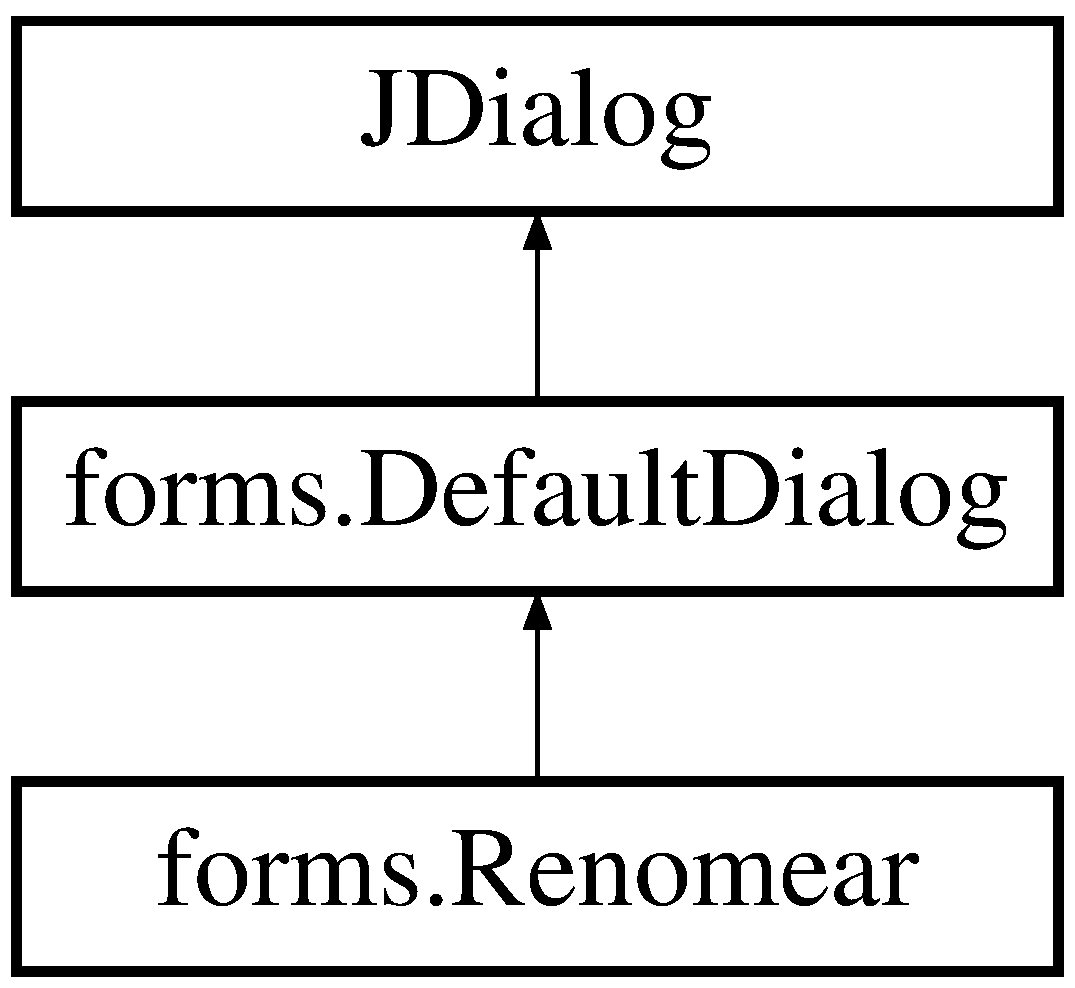
\includegraphics[height=3.000000cm]{classforms_1_1_renomear}
\end{center}
\end{figure}
\subsection*{Public Member Functions}
\begin{DoxyCompactItemize}
\item 
\hyperlink{classforms_1_1_renomear_aa8ba879ea70a7e2a39452c1c8d6b8ded}{Renomear} (java.\+awt.\+Frame parent, boolean modal)
\end{DoxyCompactItemize}
\subsection*{Static Public Member Functions}
\begin{DoxyCompactItemize}
\item 
static void \hyperlink{classforms_1_1_renomear_aedef87434fb9f9311e047557a7643c41}{main} (String args\mbox{[}$\,$\mbox{]})
\end{DoxyCompactItemize}
\subsection*{Additional Inherited Members}


\subsection{Detailed Description}
\begin{DoxyAuthor}{Author}
Matheus 
\end{DoxyAuthor}


\subsection{Constructor \& Destructor Documentation}
\hypertarget{classforms_1_1_renomear_aa8ba879ea70a7e2a39452c1c8d6b8ded}{\index{forms\+::\+Renomear@{forms\+::\+Renomear}!Renomear@{Renomear}}
\index{Renomear@{Renomear}!forms\+::\+Renomear@{forms\+::\+Renomear}}
\subsubsection[{Renomear}]{\setlength{\rightskip}{0pt plus 5cm}forms.\+Renomear.\+Renomear (
\begin{DoxyParamCaption}
\item[{java.\+awt.\+Frame}]{parent, }
\item[{boolean}]{modal}
\end{DoxyParamCaption}
)}}\label{classforms_1_1_renomear_aa8ba879ea70a7e2a39452c1c8d6b8ded}
Creates new form \hyperlink{classforms_1_1_renomear}{Renomear} 

\subsection{Member Function Documentation}
\hypertarget{classforms_1_1_renomear_aedef87434fb9f9311e047557a7643c41}{\index{forms\+::\+Renomear@{forms\+::\+Renomear}!main@{main}}
\index{main@{main}!forms\+::\+Renomear@{forms\+::\+Renomear}}
\subsubsection[{main}]{\setlength{\rightskip}{0pt plus 5cm}static void forms.\+Renomear.\+main (
\begin{DoxyParamCaption}
\item[{String}]{args\mbox{[}$\,$\mbox{]}}
\end{DoxyParamCaption}
)\hspace{0.3cm}{\ttfamily [static]}}}\label{classforms_1_1_renomear_aedef87434fb9f9311e047557a7643c41}

\begin{DoxyParams}{Parameters}
{\em args} & the command line arguments \\
\hline
\end{DoxyParams}


The documentation for this class was generated from the following file\+:\begin{DoxyCompactItemize}
\item 
src/forms/Renomear.\+java\end{DoxyCompactItemize}

\hypertarget{classservidor_1_1_sistema_arquivo}{\section{servidor.\+Sistema\+Arquivo Class Reference}
\label{classservidor_1_1_sistema_arquivo}\index{servidor.\+Sistema\+Arquivo@{servidor.\+Sistema\+Arquivo}}
}
Inheritance diagram for servidor.\+Sistema\+Arquivo\+:\begin{figure}[H]
\begin{center}
\leavevmode
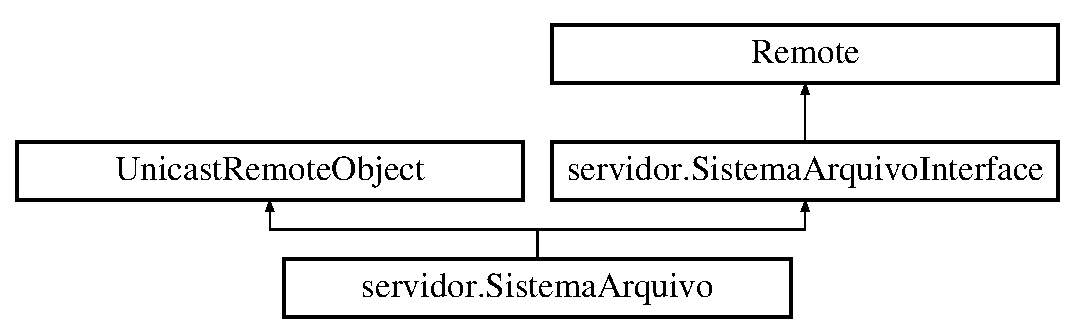
\includegraphics[height=3.000000cm]{classservidor_1_1_sistema_arquivo}
\end{center}
\end{figure}
\subsection*{Classes}
\begin{DoxyCompactItemize}
\item 
class \hyperlink{classservidor_1_1_sistema_arquivo_1_1_heartbeat}{Heartbeat}
\item 
class {\bfseries My\+Policy}
\end{DoxyCompactItemize}
\subsection*{Public Member Functions}
\begin{DoxyCompactItemize}
\item 
\hypertarget{classservidor_1_1_sistema_arquivo_a00a6f007cd7758829f5c3c83a0234c7a}{{\bfseries Sistema\+Arquivo} (String string)  throws Remote\+Exception }\label{classservidor_1_1_sistema_arquivo_a00a6f007cd7758829f5c3c83a0234c7a}

\item 
boolean \hyperlink{classservidor_1_1_sistema_arquivo_afa7146862daa7c0f38a1694d3073a7fe}{criar\+Arquivo} (String caminho, \hyperlink{classmodel_1_1_arquivo}{Arquivo} arquivo, String nome\+Usuario)  throws Remote\+Exception, X\+Path\+Expression\+Exception 
\item 
boolean \hyperlink{classservidor_1_1_sistema_arquivo_a54fff1b72f54a538c624c40f239d18f6}{criar\+Pasta} (String caminho, String nome\+Usuario)  throws Remote\+Exception, X\+Path\+Expression\+Exception 
\item 
Document \hyperlink{classservidor_1_1_sistema_arquivo_abcead514a91516e7db1b794afe5fdf14}{pedir\+X\+M\+L} (String nome\+Usuario)
\item 
boolean \hyperlink{classservidor_1_1_sistema_arquivo_a66be9b03399b2765ade1f5c2d39877a2}{deletar\+Arquivo} (String caminho, String nome\+Usuario)  throws Remote\+Exception, X\+Path\+Expression\+Exception 
\item 
boolean \hyperlink{classservidor_1_1_sistema_arquivo_a9ca48ba1937eca40566d38aadb888b12}{deletar\+Pasta} (String caminho, String nome\+Usuario)  throws Remote\+Exception, X\+Path\+Expression\+Exception 
\item 
boolean \hyperlink{classservidor_1_1_sistema_arquivo_ae0423e77b2ed7e597c8eeb292210631f}{renomear\+Arquivo} (String caminho\+Origem, String novo\+Nome, String nome\+Usuario)  throws Remote\+Exception, X\+Path\+Expression\+Exception 
\item 
boolean \hyperlink{classservidor_1_1_sistema_arquivo_a323b2d7c1e5c7c364029bb6557a6f444}{mover\+Arquivo} (String caminho\+Origem, String caminho\+Destino, String nome\+Usuario)  throws Remote\+Exception, X\+Path\+Expression\+Exception 
\item 
boolean \hyperlink{classservidor_1_1_sistema_arquivo_a52d97f440af51e6e7a8673627c9c99a1}{mover\+Pasta} (String caminho\+Origem, String caminho\+Destino, String nome\+Usuario)  throws Remote\+Exception, X\+Path\+Expression\+Exception 
\item 
boolean \hyperlink{classservidor_1_1_sistema_arquivo_abe818245ebc8bfdef68e6216b0395d50}{copiar\+Arquivo} (String caminho\+Origem, String caminho\+Destino, String nome\+Usuario)  throws Remote\+Exception, X\+Path\+Expression\+Exception 
\item 
boolean \hyperlink{classservidor_1_1_sistema_arquivo_ac33210e1f9a88aa0ac8dcfc0169838a6}{copiar\+Pasta} (String caminho\+Origem, String caminho\+Destino, String nome\+Usuario)  throws Remote\+Exception, X\+Path\+Expression\+Exception 
\item 
String \hyperlink{classservidor_1_1_sistema_arquivo_a71a3848f1d40dbcdf0625fd066435a73}{ler\+Arquivo} (String caminho, String nome\+Usuario)  throws Remote\+Exception, X\+Path\+Expression\+Exception 
\item 
boolean \hyperlink{classservidor_1_1_sistema_arquivo_a88d924eb3b3fa3cb1978478a9593e3fb}{escrever\+Arquivo} (String caminho, String texto, String nome\+Usuario)  throws Remote\+Exception, X\+Path\+Expression\+Exception 
\item 
\hyperlink{classmodel_1_1_arquivo}{Arquivo} \hyperlink{classservidor_1_1_sistema_arquivo_acdc517b4cd0f061d0f2c6ed9ea2a2911}{get\+Arquivo} (String caminho, String nome\+Usuario)  throws Remote\+Exception, X\+Path\+Expression\+Exception 
\item 
List$<$ \hyperlink{classmodel_1_1_arquivo}{Arquivo} $>$ \hyperlink{classservidor_1_1_sistema_arquivo_a73d86137128b1cd630042742cc7f9192}{backup\+Arquivos\+Usuario} (String nome\+Usuario)  throws Remote\+Exception, X\+Path\+Expression\+Exception 
\item 
void \hyperlink{classservidor_1_1_sistema_arquivo_a9665a2e279240dac472a74fe3446851d}{unlock} (String caminho, String nome\+Usuario)  throws Remote\+Exception, X\+Path\+Expression\+Exception 
\item 
\hypertarget{classservidor_1_1_sistema_arquivo_a8efeadfedc74fd9858d06c6d3be9cf8c}{List$<$ String $>$ {\bfseries get\+Usuarios} ()}\label{classservidor_1_1_sistema_arquivo_a8efeadfedc74fd9858d06c6d3be9cf8c}

\end{DoxyCompactItemize}
\subsection*{Static Public Member Functions}
\begin{DoxyCompactItemize}
\item 
\hypertarget{classservidor_1_1_sistema_arquivo_a5b4400e9b1506f105fff97d8be9d1a82}{static void {\bfseries main} (String\mbox{[}$\,$\mbox{]} args)}\label{classservidor_1_1_sistema_arquivo_a5b4400e9b1506f105fff97d8be9d1a82}

\end{DoxyCompactItemize}


\subsection{Member Function Documentation}
\hypertarget{classservidor_1_1_sistema_arquivo_a73d86137128b1cd630042742cc7f9192}{\index{servidor\+::\+Sistema\+Arquivo@{servidor\+::\+Sistema\+Arquivo}!backup\+Arquivos\+Usuario@{backup\+Arquivos\+Usuario}}
\index{backup\+Arquivos\+Usuario@{backup\+Arquivos\+Usuario}!servidor\+::\+Sistema\+Arquivo@{servidor\+::\+Sistema\+Arquivo}}
\subsubsection[{backup\+Arquivos\+Usuario}]{\setlength{\rightskip}{0pt plus 5cm}List$<${\bf Arquivo}$>$ servidor.\+Sistema\+Arquivo.\+backup\+Arquivos\+Usuario (
\begin{DoxyParamCaption}
\item[{String}]{nome\+Usuario}
\end{DoxyParamCaption}
) throws Remote\+Exception, X\+Path\+Expression\+Exception}}\label{classservidor_1_1_sistema_arquivo_a73d86137128b1cd630042742cc7f9192}

\begin{DoxyParams}{Parameters}
{\em nome\+Usuario} & String -\/nome do usuario que se deseja realizar o backup \\
\hline
\end{DoxyParams}
\begin{DoxyReturn}{Returns}
List$<$\+Arquivo$>$ -\/ retorna uma lista com objetos do tipo Arquivo, com os arquivos do usuario 
\end{DoxyReturn}

\begin{DoxyExceptions}{Exceptions}
{\em Remote\+Exception} & \\
\hline
{\em X\+Path\+Expression\+Exception} & \\
\hline
\end{DoxyExceptions}


Implements \hyperlink{interfaceservidor_1_1_sistema_arquivo_interface_a208daf85a9c8026080aa6b389d420339}{servidor.\+Sistema\+Arquivo\+Interface}.

\hypertarget{classservidor_1_1_sistema_arquivo_abe818245ebc8bfdef68e6216b0395d50}{\index{servidor\+::\+Sistema\+Arquivo@{servidor\+::\+Sistema\+Arquivo}!copiar\+Arquivo@{copiar\+Arquivo}}
\index{copiar\+Arquivo@{copiar\+Arquivo}!servidor\+::\+Sistema\+Arquivo@{servidor\+::\+Sistema\+Arquivo}}
\subsubsection[{copiar\+Arquivo}]{\setlength{\rightskip}{0pt plus 5cm}boolean servidor.\+Sistema\+Arquivo.\+copiar\+Arquivo (
\begin{DoxyParamCaption}
\item[{String}]{caminho\+Origem, }
\item[{String}]{caminho\+Destino, }
\item[{String}]{nome\+Usuario}
\end{DoxyParamCaption}
) throws Remote\+Exception, X\+Path\+Expression\+Exception}}\label{classservidor_1_1_sistema_arquivo_abe818245ebc8bfdef68e6216b0395d50}
Copia um arquivo, dado um caminho de origem, onde o ultimo nome após a \char`\"{}/\char`\"{} é o nome do arquivo, para o caminho de destino


\begin{DoxyParams}{Parameters}
{\em caminho\+Origem} & String -\/ caminho de origem do arquivo a ser copiado, concatenado com \char`\"{}/\char`\"{} e o nome do arquivo \\
\hline
{\em caminho\+Destino} & String -\/ caminho de destino do arquivo \\
\hline
{\em nome\+Usuario} & String -\/ nome do usuário para salvar o X\+M\+L \\
\hline
\end{DoxyParams}
\begin{DoxyReturn}{Returns}
boolean -\/ true caso seja possivel mover o arquivo ou false caso não seja possível 
\end{DoxyReturn}

\begin{DoxyExceptions}{Exceptions}
{\em Remote\+Exception} & \\
\hline
{\em javax.\+xml.\+xpath.\+X\+Path\+Expression\+Exception} & \\
\hline
\end{DoxyExceptions}


Implements \hyperlink{interfaceservidor_1_1_sistema_arquivo_interface_a386c5f49538f37522be89af4ca35d245}{servidor.\+Sistema\+Arquivo\+Interface}.

\hypertarget{classservidor_1_1_sistema_arquivo_ac33210e1f9a88aa0ac8dcfc0169838a6}{\index{servidor\+::\+Sistema\+Arquivo@{servidor\+::\+Sistema\+Arquivo}!copiar\+Pasta@{copiar\+Pasta}}
\index{copiar\+Pasta@{copiar\+Pasta}!servidor\+::\+Sistema\+Arquivo@{servidor\+::\+Sistema\+Arquivo}}
\subsubsection[{copiar\+Pasta}]{\setlength{\rightskip}{0pt plus 5cm}boolean servidor.\+Sistema\+Arquivo.\+copiar\+Pasta (
\begin{DoxyParamCaption}
\item[{String}]{caminho\+Origem, }
\item[{String}]{caminho\+Destino, }
\item[{String}]{nome\+Usuario}
\end{DoxyParamCaption}
) throws Remote\+Exception, X\+Path\+Expression\+Exception}}\label{classservidor_1_1_sistema_arquivo_ac33210e1f9a88aa0ac8dcfc0169838a6}
Copia uma pasta recursivamente, dado um caminho de origem, onde o ultimo nome após a \char`\"{}/\char`\"{} é a pasta a ser copiada, para o caminho de destino


\begin{DoxyParams}{Parameters}
{\em caminho\+Origem} & String -\/ caminho de origem da pasta a ser copiada, concatenado com \char`\"{}/\char`\"{} \\
\hline
{\em caminho\+Destino} & String -\/ caminho de destino da pasta \\
\hline
{\em nome\+Usuario} & String -\/ nome do usuário para salvar o X\+M\+L \\
\hline
\end{DoxyParams}
\begin{DoxyReturn}{Returns}
boolean -\/ true caso seja possivel mover o arquivo ou false caso não seja possível 
\end{DoxyReturn}

\begin{DoxyExceptions}{Exceptions}
{\em Remote\+Exception} & \\
\hline
{\em javax.\+xml.\+xpath.\+X\+Path\+Expression\+Exception} & \\
\hline
\end{DoxyExceptions}


Implements \hyperlink{interfaceservidor_1_1_sistema_arquivo_interface_ab7818dbb84f0d389cfbf10f0f0bb9580}{servidor.\+Sistema\+Arquivo\+Interface}.

\hypertarget{classservidor_1_1_sistema_arquivo_afa7146862daa7c0f38a1694d3073a7fe}{\index{servidor\+::\+Sistema\+Arquivo@{servidor\+::\+Sistema\+Arquivo}!criar\+Arquivo@{criar\+Arquivo}}
\index{criar\+Arquivo@{criar\+Arquivo}!servidor\+::\+Sistema\+Arquivo@{servidor\+::\+Sistema\+Arquivo}}
\subsubsection[{criar\+Arquivo}]{\setlength{\rightskip}{0pt plus 5cm}boolean servidor.\+Sistema\+Arquivo.\+criar\+Arquivo (
\begin{DoxyParamCaption}
\item[{String}]{caminho, }
\item[{{\bf Arquivo}}]{arquivo, }
\item[{String}]{nome\+Usuario}
\end{DoxyParamCaption}
) throws Remote\+Exception, X\+Path\+Expression\+Exception}}\label{classservidor_1_1_sistema_arquivo_afa7146862daa7c0f38a1694d3073a7fe}
Cria um arquivo passando o caminho do arquivo, separado por barra, onde o ultimo nome, após a ultima barra, corresponde ao nome do arquivo


\begin{DoxyParams}{Parameters}
{\em caminho} & String -\/ caminho onde será criado o arquivo, concatenado com \char`\"{}/\char`\"{} e o nome do arquivo \\
\hline
{\em arquivo} & Arquivo -\/ Objeto do arquivo a ser salvo no disco \\
\hline
{\em nome\+Usuario} & String -\/ nome do usuário para salvar o X\+M\+L \\
\hline
\end{DoxyParams}
\begin{DoxyReturn}{Returns}
boolean -\/ true caso seja possivel criar o arquivo ou false caso já exista um arquivo com o nome 
\end{DoxyReturn}

\begin{DoxyExceptions}{Exceptions}
{\em Remote\+Exception} & \\
\hline
{\em javax.\+xml.\+xpath.\+X\+Path\+Expression\+Exception} & \\
\hline
\end{DoxyExceptions}


Implements \hyperlink{interfaceservidor_1_1_sistema_arquivo_interface_a8668540815b2886b3816ac23e3e24740}{servidor.\+Sistema\+Arquivo\+Interface}.

\hypertarget{classservidor_1_1_sistema_arquivo_a54fff1b72f54a538c624c40f239d18f6}{\index{servidor\+::\+Sistema\+Arquivo@{servidor\+::\+Sistema\+Arquivo}!criar\+Pasta@{criar\+Pasta}}
\index{criar\+Pasta@{criar\+Pasta}!servidor\+::\+Sistema\+Arquivo@{servidor\+::\+Sistema\+Arquivo}}
\subsubsection[{criar\+Pasta}]{\setlength{\rightskip}{0pt plus 5cm}boolean servidor.\+Sistema\+Arquivo.\+criar\+Pasta (
\begin{DoxyParamCaption}
\item[{String}]{caminho, }
\item[{String}]{nome\+Usuario}
\end{DoxyParamCaption}
) throws Remote\+Exception, X\+Path\+Expression\+Exception}}\label{classservidor_1_1_sistema_arquivo_a54fff1b72f54a538c624c40f239d18f6}
Cria uma pasta dado um caminho, onde o último nome, após a última barra, corresponde ao nome da pasta


\begin{DoxyParams}{Parameters}
{\em caminho} & String -\/ caminho onde será criado a pasta, concatenado com \char`\"{}/\char`\"{} e o nome da pasta
\begin{DoxyItemize}
\item 
\end{DoxyItemize}\\
\hline
{\em nome\+Usuario} & String -\/ nome do usuário para salvar o X\+M\+L \\
\hline
\end{DoxyParams}
\begin{DoxyReturn}{Returns}
boolean -\/ true caso seja possivel criar a pasta ou false caso já exista uma pasta com o mesmo nome 
\end{DoxyReturn}

\begin{DoxyExceptions}{Exceptions}
{\em Remote\+Exception} & \\
\hline
{\em javax.\+xml.\+xpath.\+X\+Path\+Expression\+Exception} & \\
\hline
\end{DoxyExceptions}


Implements \hyperlink{interfaceservidor_1_1_sistema_arquivo_interface_a46a7a411f21d0db4cad12e07425a2259}{servidor.\+Sistema\+Arquivo\+Interface}.

\hypertarget{classservidor_1_1_sistema_arquivo_a66be9b03399b2765ade1f5c2d39877a2}{\index{servidor\+::\+Sistema\+Arquivo@{servidor\+::\+Sistema\+Arquivo}!deletar\+Arquivo@{deletar\+Arquivo}}
\index{deletar\+Arquivo@{deletar\+Arquivo}!servidor\+::\+Sistema\+Arquivo@{servidor\+::\+Sistema\+Arquivo}}
\subsubsection[{deletar\+Arquivo}]{\setlength{\rightskip}{0pt plus 5cm}boolean servidor.\+Sistema\+Arquivo.\+deletar\+Arquivo (
\begin{DoxyParamCaption}
\item[{String}]{caminho, }
\item[{String}]{nome\+Usuario}
\end{DoxyParamCaption}
) throws Remote\+Exception, X\+Path\+Expression\+Exception}}\label{classservidor_1_1_sistema_arquivo_a66be9b03399b2765ade1f5c2d39877a2}
Deleta um arquivo passando o caminho do arquivo, separado por barra, onde o ultimo nome, após a ultima barra, corresponde ao nome do arquivo


\begin{DoxyParams}{Parameters}
{\em caminho} & String -\/ caminho do arquivo a ser deletado, concatenado com \char`\"{}/\char`\"{} e o nome do arquivo
\begin{DoxyItemize}
\item 
\end{DoxyItemize}\\
\hline
{\em nome\+Usuario} & String -\/ nome do usuário para salvar o X\+M\+L \\
\hline
\end{DoxyParams}
\begin{DoxyReturn}{Returns}
boolean -\/ true caso seja possivel deletar o arquivo ou false caso não seja possível 
\end{DoxyReturn}

\begin{DoxyExceptions}{Exceptions}
{\em Remote\+Exception} & \\
\hline
{\em javax.\+xml.\+xpath.\+X\+Path\+Expression\+Exception} & \\
\hline
\end{DoxyExceptions}


Implements \hyperlink{interfaceservidor_1_1_sistema_arquivo_interface_afb7dfa9a67c813d586d9fbce4fb9e001}{servidor.\+Sistema\+Arquivo\+Interface}.

\hypertarget{classservidor_1_1_sistema_arquivo_a9ca48ba1937eca40566d38aadb888b12}{\index{servidor\+::\+Sistema\+Arquivo@{servidor\+::\+Sistema\+Arquivo}!deletar\+Pasta@{deletar\+Pasta}}
\index{deletar\+Pasta@{deletar\+Pasta}!servidor\+::\+Sistema\+Arquivo@{servidor\+::\+Sistema\+Arquivo}}
\subsubsection[{deletar\+Pasta}]{\setlength{\rightskip}{0pt plus 5cm}boolean servidor.\+Sistema\+Arquivo.\+deletar\+Pasta (
\begin{DoxyParamCaption}
\item[{String}]{caminho, }
\item[{String}]{nome\+Usuario}
\end{DoxyParamCaption}
) throws Remote\+Exception, X\+Path\+Expression\+Exception}}\label{classservidor_1_1_sistema_arquivo_a9ca48ba1937eca40566d38aadb888b12}
Deleta uma pasta dado seu caminho, separado por barra, onde o ultimo nome, após a ultima barra, corresponde ao nome da pasta


\begin{DoxyParams}{Parameters}
{\em caminho} & String -\/ caminho do arquivo a ser deletado, concatenado com \char`\"{}/\char`\"{} e o nome do arquivo \\
\hline
{\em nome\+Usuario} & String -\/ nome do usuário para salvar o X\+M\+L \\
\hline
\end{DoxyParams}
\begin{DoxyReturn}{Returns}
boolean -\/ true caso seja possivel deletar o arquivo ou false caso não seja possível 
\end{DoxyReturn}

\begin{DoxyExceptions}{Exceptions}
{\em Remote\+Exception} & \\
\hline
{\em javax.\+xml.\+xpath.\+X\+Path\+Expression\+Exception} & \\
\hline
\end{DoxyExceptions}


Implements \hyperlink{interfaceservidor_1_1_sistema_arquivo_interface_ad24ed755bdc26c9e6bcfab426d3649aa}{servidor.\+Sistema\+Arquivo\+Interface}.

\hypertarget{classservidor_1_1_sistema_arquivo_a88d924eb3b3fa3cb1978478a9593e3fb}{\index{servidor\+::\+Sistema\+Arquivo@{servidor\+::\+Sistema\+Arquivo}!escrever\+Arquivo@{escrever\+Arquivo}}
\index{escrever\+Arquivo@{escrever\+Arquivo}!servidor\+::\+Sistema\+Arquivo@{servidor\+::\+Sistema\+Arquivo}}
\subsubsection[{escrever\+Arquivo}]{\setlength{\rightskip}{0pt plus 5cm}boolean servidor.\+Sistema\+Arquivo.\+escrever\+Arquivo (
\begin{DoxyParamCaption}
\item[{String}]{caminho, }
\item[{String}]{texto, }
\item[{String}]{nome\+Usuario}
\end{DoxyParamCaption}
) throws Remote\+Exception, X\+Path\+Expression\+Exception}}\label{classservidor_1_1_sistema_arquivo_a88d924eb3b3fa3cb1978478a9593e3fb}
Escreve no final do arquivo indicado ao final do caminho


\begin{DoxyParams}{Parameters}
{\em caminho} & String -\/ caminho para o arquivo \\
\hline
{\em texto} & String -\/ texto a ser escrito no final do arquivo \\
\hline
{\em nome\+Usuario} & String -\/ nome do usuário para salvar o X\+M\+L \\
\hline
\end{DoxyParams}
\begin{DoxyReturn}{Returns}
boolean -\/ retorna true caso o arquivo seja alterado com sucesso, caso contrário retorna falso 
\end{DoxyReturn}

\begin{DoxyExceptions}{Exceptions}
{\em Remote\+Exception} & \\
\hline
{\em javax.\+xml.\+xpath.\+X\+Path\+Expression\+Exception} & \\
\hline
\end{DoxyExceptions}


Implements \hyperlink{interfaceservidor_1_1_sistema_arquivo_interface_a028895ffa088ee8eec9ee83768996b44}{servidor.\+Sistema\+Arquivo\+Interface}.

\hypertarget{classservidor_1_1_sistema_arquivo_acdc517b4cd0f061d0f2c6ed9ea2a2911}{\index{servidor\+::\+Sistema\+Arquivo@{servidor\+::\+Sistema\+Arquivo}!get\+Arquivo@{get\+Arquivo}}
\index{get\+Arquivo@{get\+Arquivo}!servidor\+::\+Sistema\+Arquivo@{servidor\+::\+Sistema\+Arquivo}}
\subsubsection[{get\+Arquivo}]{\setlength{\rightskip}{0pt plus 5cm}{\bf Arquivo} servidor.\+Sistema\+Arquivo.\+get\+Arquivo (
\begin{DoxyParamCaption}
\item[{String}]{caminho, }
\item[{String}]{nome\+Usuario}
\end{DoxyParamCaption}
) throws Remote\+Exception, X\+Path\+Expression\+Exception}}\label{classservidor_1_1_sistema_arquivo_acdc517b4cd0f061d0f2c6ed9ea2a2911}
Retorna um objeto Arquivo com as informações referentes ao arquivo no final do caminho


\begin{DoxyParams}{Parameters}
{\em caminho} & String -\/ caminho para o arquivo que se deseja as informações \\
\hline
{\em nome\+Usuario} & String -\/ nome do usuario \\
\hline
\end{DoxyParams}
\begin{DoxyReturn}{Returns}
Arquivo -\/ retorna um objeto com as informações referentes ao arquivo 
\end{DoxyReturn}

\begin{DoxyExceptions}{Exceptions}
{\em Remote\+Exception} & \\
\hline
{\em javax.\+xml.\+xpath.\+X\+Path\+Expression\+Exception} & \\
\hline
\end{DoxyExceptions}


Implements \hyperlink{interfaceservidor_1_1_sistema_arquivo_interface_aa8a1fa4f295b2f50f0b099182493e81e}{servidor.\+Sistema\+Arquivo\+Interface}.

\hypertarget{classservidor_1_1_sistema_arquivo_a71a3848f1d40dbcdf0625fd066435a73}{\index{servidor\+::\+Sistema\+Arquivo@{servidor\+::\+Sistema\+Arquivo}!ler\+Arquivo@{ler\+Arquivo}}
\index{ler\+Arquivo@{ler\+Arquivo}!servidor\+::\+Sistema\+Arquivo@{servidor\+::\+Sistema\+Arquivo}}
\subsubsection[{ler\+Arquivo}]{\setlength{\rightskip}{0pt plus 5cm}String servidor.\+Sistema\+Arquivo.\+ler\+Arquivo (
\begin{DoxyParamCaption}
\item[{String}]{caminho, }
\item[{String}]{nome\+Usuario}
\end{DoxyParamCaption}
) throws Remote\+Exception, X\+Path\+Expression\+Exception}}\label{classservidor_1_1_sistema_arquivo_a71a3848f1d40dbcdf0625fd066435a73}
Lê o conteudo do arquivo ao final do caminho


\begin{DoxyParams}{Parameters}
{\em caminho} & String -\/ caminho para o arquivo \\
\hline
{\em nome\+Usuario} & String -\/ nome do usuario \\
\hline
\end{DoxyParams}
\begin{DoxyReturn}{Returns}
String -\/ retorna o conteudo do arquivo em forma de texto 
\end{DoxyReturn}

\begin{DoxyExceptions}{Exceptions}
{\em Remote\+Exception} & \\
\hline
{\em javax.\+xml.\+xpath.\+X\+Path\+Expression\+Exception} & \\
\hline
\end{DoxyExceptions}


Implements \hyperlink{interfaceservidor_1_1_sistema_arquivo_interface_a528fb29aaa4b74c7cdfec5dad5803329}{servidor.\+Sistema\+Arquivo\+Interface}.

\hypertarget{classservidor_1_1_sistema_arquivo_a323b2d7c1e5c7c364029bb6557a6f444}{\index{servidor\+::\+Sistema\+Arquivo@{servidor\+::\+Sistema\+Arquivo}!mover\+Arquivo@{mover\+Arquivo}}
\index{mover\+Arquivo@{mover\+Arquivo}!servidor\+::\+Sistema\+Arquivo@{servidor\+::\+Sistema\+Arquivo}}
\subsubsection[{mover\+Arquivo}]{\setlength{\rightskip}{0pt plus 5cm}boolean servidor.\+Sistema\+Arquivo.\+mover\+Arquivo (
\begin{DoxyParamCaption}
\item[{String}]{caminho\+Origem, }
\item[{String}]{caminho\+Destino, }
\item[{String}]{nome\+Usuario}
\end{DoxyParamCaption}
) throws Remote\+Exception, X\+Path\+Expression\+Exception}}\label{classservidor_1_1_sistema_arquivo_a323b2d7c1e5c7c364029bb6557a6f444}
Move um arquivo, dado um caminho de origem, onde o ultimo nome após a \char`\"{}/\char`\"{} é o nome do arquivo, para o caminho de destino


\begin{DoxyParams}{Parameters}
{\em caminho\+Origem} & String -\/ caminho de origem do arquivo a ser movido, concatenado com \char`\"{}/\char`\"{} e o nome do arquivo \\
\hline
{\em caminho\+Destino} & -\/ caminho de destino do arquivo. \\
\hline
{\em nome\+Usuario} & String -\/ nome do usuário para salvar o X\+M\+L \\
\hline
\end{DoxyParams}
\begin{DoxyReturn}{Returns}
boolean -\/ true caso seja possivel mover o arquivo ou false caso não seja possível 
\end{DoxyReturn}

\begin{DoxyExceptions}{Exceptions}
{\em Remote\+Exception} & \\
\hline
{\em javax.\+xml.\+xpath.\+X\+Path\+Expression\+Exception} & \\
\hline
\end{DoxyExceptions}


Implements \hyperlink{interfaceservidor_1_1_sistema_arquivo_interface_a187abef3707033620038ceaf7bf61862}{servidor.\+Sistema\+Arquivo\+Interface}.

\hypertarget{classservidor_1_1_sistema_arquivo_a52d97f440af51e6e7a8673627c9c99a1}{\index{servidor\+::\+Sistema\+Arquivo@{servidor\+::\+Sistema\+Arquivo}!mover\+Pasta@{mover\+Pasta}}
\index{mover\+Pasta@{mover\+Pasta}!servidor\+::\+Sistema\+Arquivo@{servidor\+::\+Sistema\+Arquivo}}
\subsubsection[{mover\+Pasta}]{\setlength{\rightskip}{0pt plus 5cm}boolean servidor.\+Sistema\+Arquivo.\+mover\+Pasta (
\begin{DoxyParamCaption}
\item[{String}]{caminho\+Origem, }
\item[{String}]{caminho\+Destino, }
\item[{String}]{nome\+Usuario}
\end{DoxyParamCaption}
) throws Remote\+Exception, X\+Path\+Expression\+Exception}}\label{classservidor_1_1_sistema_arquivo_a52d97f440af51e6e7a8673627c9c99a1}
Move uma pasta, dado um caminho de origem, onde o ultimo nome após a \char`\"{}/\char`\"{} é o nome da pasta, para o caminho de destino


\begin{DoxyParams}{Parameters}
{\em caminho\+Origem} & String -\/ caminho de origem da pasta a ser movida, concatenado com \char`\"{}/\char`\"{} \\
\hline
{\em caminho\+Destino} & -\/ caminho de destino do arquivo. \\
\hline
{\em nome\+Usuario} & String -\/ nome do usuário para salvar o X\+M\+L \\
\hline
\end{DoxyParams}
\begin{DoxyReturn}{Returns}
boolean -\/ true caso seja possivel mover a pasta ou false caso não seja possível 
\end{DoxyReturn}

\begin{DoxyExceptions}{Exceptions}
{\em Remote\+Exception} & \\
\hline
{\em javax.\+xml.\+xpath.\+X\+Path\+Expression\+Exception} & \\
\hline
\end{DoxyExceptions}


Implements \hyperlink{interfaceservidor_1_1_sistema_arquivo_interface_a5cb77a26cf0c6ec0868473aca67b15ca}{servidor.\+Sistema\+Arquivo\+Interface}.

\hypertarget{classservidor_1_1_sistema_arquivo_abcead514a91516e7db1b794afe5fdf14}{\index{servidor\+::\+Sistema\+Arquivo@{servidor\+::\+Sistema\+Arquivo}!pedir\+X\+M\+L@{pedir\+X\+M\+L}}
\index{pedir\+X\+M\+L@{pedir\+X\+M\+L}!servidor\+::\+Sistema\+Arquivo@{servidor\+::\+Sistema\+Arquivo}}
\subsubsection[{pedir\+X\+M\+L}]{\setlength{\rightskip}{0pt plus 5cm}Document servidor.\+Sistema\+Arquivo.\+pedir\+X\+M\+L (
\begin{DoxyParamCaption}
\item[{String}]{nome\+Usuario}
\end{DoxyParamCaption}
)}}\label{classservidor_1_1_sistema_arquivo_abcead514a91516e7db1b794afe5fdf14}

\begin{DoxyParams}{Parameters}
{\em nome\+Usuario} & String -\/ nome do usuario que se deseja o xml \\
\hline
\end{DoxyParams}
\begin{DoxyReturn}{Returns}
Document -\/ xml com a arvore de arquivos do usuario 
\end{DoxyReturn}

\begin{DoxyExceptions}{Exceptions}
{\em Remote\+Exception} & \\
\hline
{\em X\+Path\+Expression\+Exception} & \\
\hline
\end{DoxyExceptions}


Implements \hyperlink{interfaceservidor_1_1_sistema_arquivo_interface_a7a35e15725ff21dbd8373742cc518b77}{servidor.\+Sistema\+Arquivo\+Interface}.

\hypertarget{classservidor_1_1_sistema_arquivo_ae0423e77b2ed7e597c8eeb292210631f}{\index{servidor\+::\+Sistema\+Arquivo@{servidor\+::\+Sistema\+Arquivo}!renomear\+Arquivo@{renomear\+Arquivo}}
\index{renomear\+Arquivo@{renomear\+Arquivo}!servidor\+::\+Sistema\+Arquivo@{servidor\+::\+Sistema\+Arquivo}}
\subsubsection[{renomear\+Arquivo}]{\setlength{\rightskip}{0pt plus 5cm}boolean servidor.\+Sistema\+Arquivo.\+renomear\+Arquivo (
\begin{DoxyParamCaption}
\item[{String}]{caminho\+Origem, }
\item[{String}]{novo\+Nome, }
\item[{String}]{nome\+Usuario}
\end{DoxyParamCaption}
) throws Remote\+Exception, X\+Path\+Expression\+Exception}}\label{classservidor_1_1_sistema_arquivo_ae0423e77b2ed7e597c8eeb292210631f}
Renomeia um arquivo passando o caminho de origem do arquivo, separado por barra, onde o ultimo nome, após a ultima barra, corresponde ao nome do arquivo. O caminho de destino corresponde ao caminho do arquivo, separado por barra, onde o ultimo nome é o novo nome do arquivo


\begin{DoxyParams}{Parameters}
{\em caminho\+Origem} & String -\/ caminho do arquivo/pasta a ser renomeado, concatenado com \char`\"{}/\char`\"{} e o nome do arquivo \\
\hline
{\em novo\+Nome} & String -\/ novo nome do arquivo/pasta \\
\hline
{\em nome\+Usuario} & String -\/ nome do usuário para salvar o X\+M\+L \\
\hline
\end{DoxyParams}
\begin{DoxyReturn}{Returns}
boolean -\/ true caso seja possivel renomear o arquivo ou false caso não seja possível 
\end{DoxyReturn}

\begin{DoxyExceptions}{Exceptions}
{\em Remote\+Exception} & \\
\hline
{\em javax.\+xml.\+xpath.\+X\+Path\+Expression\+Exception} & \\
\hline
\end{DoxyExceptions}


Implements \hyperlink{interfaceservidor_1_1_sistema_arquivo_interface_a38ac4858f2f0e0743dea54983b24b860}{servidor.\+Sistema\+Arquivo\+Interface}.

\hypertarget{classservidor_1_1_sistema_arquivo_a9665a2e279240dac472a74fe3446851d}{\index{servidor\+::\+Sistema\+Arquivo@{servidor\+::\+Sistema\+Arquivo}!unlock@{unlock}}
\index{unlock@{unlock}!servidor\+::\+Sistema\+Arquivo@{servidor\+::\+Sistema\+Arquivo}}
\subsubsection[{unlock}]{\setlength{\rightskip}{0pt plus 5cm}void servidor.\+Sistema\+Arquivo.\+unlock (
\begin{DoxyParamCaption}
\item[{String}]{caminho, }
\item[{String}]{nome\+Usuario}
\end{DoxyParamCaption}
) throws Remote\+Exception, X\+Path\+Expression\+Exception}}\label{classservidor_1_1_sistema_arquivo_a9665a2e279240dac472a74fe3446851d}
Destrava o arquivo representado pelo parâmetro caminho do usuário 
\begin{DoxyParams}{Parameters}
{\em caminho} & String -\/ caminho do arquivo a ser destravado \\
\hline
{\em nome\+Usuario} & String -\/ nome do usuario que se deseja o xml \\
\hline
\end{DoxyParams}

\begin{DoxyExceptions}{Exceptions}
{\em Remote\+Exception} & \\
\hline
{\em X\+Path\+Expression\+Exception} & \\
\hline
\end{DoxyExceptions}


Implements \hyperlink{interfaceservidor_1_1_sistema_arquivo_interface_a29ea9727745ef7e9f6d554ae3cad79cb}{servidor.\+Sistema\+Arquivo\+Interface}.



The documentation for this class was generated from the following file\+:\begin{DoxyCompactItemize}
\item 
src/servidor/Sistema\+Arquivo.\+java\end{DoxyCompactItemize}

\hypertarget{interfaceservidor_1_1_sistema_arquivo_interface}{\section{servidor.\+Sistema\+Arquivo\+Interface Interface Reference}
\label{interfaceservidor_1_1_sistema_arquivo_interface}\index{servidor.\+Sistema\+Arquivo\+Interface@{servidor.\+Sistema\+Arquivo\+Interface}}
}
Inheritance diagram for servidor.\+Sistema\+Arquivo\+Interface\+:\begin{figure}[H]
\begin{center}
\leavevmode
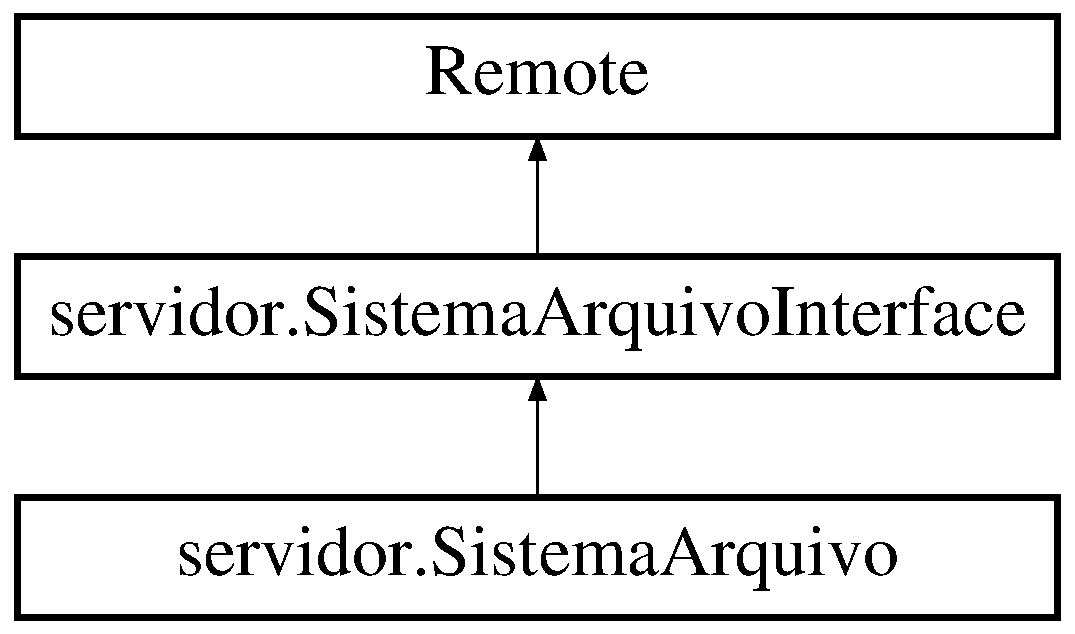
\includegraphics[height=3.000000cm]{interfaceservidor_1_1_sistema_arquivo_interface}
\end{center}
\end{figure}
\subsection*{Public Member Functions}
\begin{DoxyCompactItemize}
\item 
boolean \hyperlink{interfaceservidor_1_1_sistema_arquivo_interface_a8668540815b2886b3816ac23e3e24740}{criar\+Arquivo} (String caminho, \hyperlink{classmodel_1_1_arquivo}{Arquivo} arquivo, String nome\+Usuario)  throws Remote\+Exception, X\+Path\+Expression\+Exception
\item 
boolean \hyperlink{interfaceservidor_1_1_sistema_arquivo_interface_a46a7a411f21d0db4cad12e07425a2259}{criar\+Pasta} (String caminho, String nome\+Usuario)  throws Remote\+Exception, X\+Path\+Expression\+Exception
\item 
boolean \hyperlink{interfaceservidor_1_1_sistema_arquivo_interface_afb7dfa9a67c813d586d9fbce4fb9e001}{deletar\+Arquivo} (String caminho, String nome\+Usuario)  throws Remote\+Exception, X\+Path\+Expression\+Exception
\item 
boolean \hyperlink{interfaceservidor_1_1_sistema_arquivo_interface_ad24ed755bdc26c9e6bcfab426d3649aa}{deletar\+Pasta} (String caminho, String nome\+Usuario)  throws Remote\+Exception, X\+Path\+Expression\+Exception
\item 
boolean \hyperlink{interfaceservidor_1_1_sistema_arquivo_interface_a38ac4858f2f0e0743dea54983b24b860}{renomear\+Arquivo} (String caminho\+Origem, String novo\+Nome, String nome\+Usuario)  throws Remote\+Exception, X\+Path\+Expression\+Exception
\item 
boolean \hyperlink{interfaceservidor_1_1_sistema_arquivo_interface_a187abef3707033620038ceaf7bf61862}{mover\+Arquivo} (String caminho\+Origem, String caminho\+Destino, String nome\+Usuario)  throws Remote\+Exception, X\+Path\+Expression\+Exception
\item 
boolean \hyperlink{interfaceservidor_1_1_sistema_arquivo_interface_a5cb77a26cf0c6ec0868473aca67b15ca}{mover\+Pasta} (String caminho\+Origem, String caminho\+Destino, String nome\+Usuario)  throws Remote\+Exception, X\+Path\+Expression\+Exception
\item 
boolean \hyperlink{interfaceservidor_1_1_sistema_arquivo_interface_a386c5f49538f37522be89af4ca35d245}{copiar\+Arquivo} (String caminho\+Origem, String caminho\+Destino, String nome\+Usuario)  throws Remote\+Exception, X\+Path\+Expression\+Exception
\item 
boolean \hyperlink{interfaceservidor_1_1_sistema_arquivo_interface_ab7818dbb84f0d389cfbf10f0f0bb9580}{copiar\+Pasta} (String caminho\+Origem, String caminho\+Destino, String nome\+Usuario)  throws Remote\+Exception, X\+Path\+Expression\+Exception
\item 
String \hyperlink{interfaceservidor_1_1_sistema_arquivo_interface_a528fb29aaa4b74c7cdfec5dad5803329}{ler\+Arquivo} (String caminho, String nome\+Usuario)  throws Remote\+Exception, X\+Path\+Expression\+Exception
\item 
boolean \hyperlink{interfaceservidor_1_1_sistema_arquivo_interface_a028895ffa088ee8eec9ee83768996b44}{escrever\+Arquivo} (String caminho, String texto, String nome\+Usuario)  throws Remote\+Exception, X\+Path\+Expression\+Exception
\item 
\hyperlink{classmodel_1_1_arquivo}{Arquivo} \hyperlink{interfaceservidor_1_1_sistema_arquivo_interface_aa8a1fa4f295b2f50f0b099182493e81e}{get\+Arquivo} (String caminho, String nome\+Usuario)  throws Remote\+Exception, X\+Path\+Expression\+Exception
\item 
List$<$ \hyperlink{classmodel_1_1_arquivo}{Arquivo} $>$ \hyperlink{interfaceservidor_1_1_sistema_arquivo_interface_a208daf85a9c8026080aa6b389d420339}{backup\+Arquivos\+Usuario} (String nome\+Usuario)  throws Remote\+Exception, X\+Path\+Expression\+Exception
\item 
Document \hyperlink{interfaceservidor_1_1_sistema_arquivo_interface_a7a35e15725ff21dbd8373742cc518b77}{pedir\+X\+M\+L} (String nome\+Usuario)  throws Remote\+Exception, X\+Path\+Expression\+Exception
\item 
void \hyperlink{interfaceservidor_1_1_sistema_arquivo_interface_a29ea9727745ef7e9f6d554ae3cad79cb}{unlock} (String caminho, String nome\+Usuario)  throws Remote\+Exception, X\+Path\+Expression\+Exception
\end{DoxyCompactItemize}


\subsection{Detailed Description}
Interface para operações basicas sobre arquivos 

\subsection{Member Function Documentation}
\hypertarget{interfaceservidor_1_1_sistema_arquivo_interface_a208daf85a9c8026080aa6b389d420339}{\index{servidor\+::\+Sistema\+Arquivo\+Interface@{servidor\+::\+Sistema\+Arquivo\+Interface}!backup\+Arquivos\+Usuario@{backup\+Arquivos\+Usuario}}
\index{backup\+Arquivos\+Usuario@{backup\+Arquivos\+Usuario}!servidor\+::\+Sistema\+Arquivo\+Interface@{servidor\+::\+Sistema\+Arquivo\+Interface}}
\subsubsection[{backup\+Arquivos\+Usuario}]{\setlength{\rightskip}{0pt plus 5cm}List$<${\bf Arquivo}$>$ servidor.\+Sistema\+Arquivo\+Interface.\+backup\+Arquivos\+Usuario (
\begin{DoxyParamCaption}
\item[{String}]{nome\+Usuario}
\end{DoxyParamCaption}
) throws Remote\+Exception, X\+Path\+Expression\+Exception}}\label{interfaceservidor_1_1_sistema_arquivo_interface_a208daf85a9c8026080aa6b389d420339}

\begin{DoxyParams}{Parameters}
{\em nome\+Usuario} & String -\/nome do usuario que se deseja realizar o backup \\
\hline
\end{DoxyParams}
\begin{DoxyReturn}{Returns}
List$<$\+Arquivo$>$ -\/ retorna uma lista com objetos do tipo Arquivo, com os arquivos do usuario 
\end{DoxyReturn}

\begin{DoxyExceptions}{Exceptions}
{\em Remote\+Exception} & \\
\hline
{\em X\+Path\+Expression\+Exception} & \\
\hline
\end{DoxyExceptions}


Implemented in \hyperlink{classservidor_1_1_sistema_arquivo_a73d86137128b1cd630042742cc7f9192}{servidor.\+Sistema\+Arquivo}.

\hypertarget{interfaceservidor_1_1_sistema_arquivo_interface_a386c5f49538f37522be89af4ca35d245}{\index{servidor\+::\+Sistema\+Arquivo\+Interface@{servidor\+::\+Sistema\+Arquivo\+Interface}!copiar\+Arquivo@{copiar\+Arquivo}}
\index{copiar\+Arquivo@{copiar\+Arquivo}!servidor\+::\+Sistema\+Arquivo\+Interface@{servidor\+::\+Sistema\+Arquivo\+Interface}}
\subsubsection[{copiar\+Arquivo}]{\setlength{\rightskip}{0pt plus 5cm}boolean servidor.\+Sistema\+Arquivo\+Interface.\+copiar\+Arquivo (
\begin{DoxyParamCaption}
\item[{String}]{caminho\+Origem, }
\item[{String}]{caminho\+Destino, }
\item[{String}]{nome\+Usuario}
\end{DoxyParamCaption}
) throws Remote\+Exception, X\+Path\+Expression\+Exception}}\label{interfaceservidor_1_1_sistema_arquivo_interface_a386c5f49538f37522be89af4ca35d245}
Copia um arquivo, dado um caminho de origem, onde o ultimo nome após a \char`\"{}/\char`\"{} é o nome do arquivo, para o caminho de destino


\begin{DoxyParams}{Parameters}
{\em caminho\+Origem} & String -\/ caminho de origem do arquivo a ser copiado, concatenado com \char`\"{}/\char`\"{} e o nome do arquivo \\
\hline
{\em caminho\+Destino} & String -\/ caminho de destino do arquivo \\
\hline
{\em nome\+Usuario} & String -\/ nome do usuário para salvar o X\+M\+L \\
\hline
\end{DoxyParams}
\begin{DoxyReturn}{Returns}
boolean -\/ true caso seja possivel mover o arquivo ou false caso não seja possível 
\end{DoxyReturn}

\begin{DoxyExceptions}{Exceptions}
{\em Remote\+Exception} & \\
\hline
{\em javax.\+xml.\+xpath.\+X\+Path\+Expression\+Exception} & \\
\hline
\end{DoxyExceptions}


Implemented in \hyperlink{classservidor_1_1_sistema_arquivo_abe818245ebc8bfdef68e6216b0395d50}{servidor.\+Sistema\+Arquivo}.

\hypertarget{interfaceservidor_1_1_sistema_arquivo_interface_ab7818dbb84f0d389cfbf10f0f0bb9580}{\index{servidor\+::\+Sistema\+Arquivo\+Interface@{servidor\+::\+Sistema\+Arquivo\+Interface}!copiar\+Pasta@{copiar\+Pasta}}
\index{copiar\+Pasta@{copiar\+Pasta}!servidor\+::\+Sistema\+Arquivo\+Interface@{servidor\+::\+Sistema\+Arquivo\+Interface}}
\subsubsection[{copiar\+Pasta}]{\setlength{\rightskip}{0pt plus 5cm}boolean servidor.\+Sistema\+Arquivo\+Interface.\+copiar\+Pasta (
\begin{DoxyParamCaption}
\item[{String}]{caminho\+Origem, }
\item[{String}]{caminho\+Destino, }
\item[{String}]{nome\+Usuario}
\end{DoxyParamCaption}
) throws Remote\+Exception, X\+Path\+Expression\+Exception}}\label{interfaceservidor_1_1_sistema_arquivo_interface_ab7818dbb84f0d389cfbf10f0f0bb9580}
Copia uma pasta recursivamente, dado um caminho de origem, onde o ultimo nome após a \char`\"{}/\char`\"{} é a pasta a ser copiada, para o caminho de destino


\begin{DoxyParams}{Parameters}
{\em caminho\+Origem} & String -\/ caminho de origem da pasta a ser copiada, concatenado com \char`\"{}/\char`\"{} \\
\hline
{\em caminho\+Destino} & String -\/ caminho de destino da pasta \\
\hline
{\em nome\+Usuario} & String -\/ nome do usuário para salvar o X\+M\+L \\
\hline
\end{DoxyParams}
\begin{DoxyReturn}{Returns}
boolean -\/ true caso seja possivel mover o arquivo ou false caso não seja possível 
\end{DoxyReturn}

\begin{DoxyExceptions}{Exceptions}
{\em Remote\+Exception} & \\
\hline
{\em javax.\+xml.\+xpath.\+X\+Path\+Expression\+Exception} & \\
\hline
\end{DoxyExceptions}


Implemented in \hyperlink{classservidor_1_1_sistema_arquivo_ac33210e1f9a88aa0ac8dcfc0169838a6}{servidor.\+Sistema\+Arquivo}.

\hypertarget{interfaceservidor_1_1_sistema_arquivo_interface_a8668540815b2886b3816ac23e3e24740}{\index{servidor\+::\+Sistema\+Arquivo\+Interface@{servidor\+::\+Sistema\+Arquivo\+Interface}!criar\+Arquivo@{criar\+Arquivo}}
\index{criar\+Arquivo@{criar\+Arquivo}!servidor\+::\+Sistema\+Arquivo\+Interface@{servidor\+::\+Sistema\+Arquivo\+Interface}}
\subsubsection[{criar\+Arquivo}]{\setlength{\rightskip}{0pt plus 5cm}boolean servidor.\+Sistema\+Arquivo\+Interface.\+criar\+Arquivo (
\begin{DoxyParamCaption}
\item[{String}]{caminho, }
\item[{{\bf Arquivo}}]{arquivo, }
\item[{String}]{nome\+Usuario}
\end{DoxyParamCaption}
) throws Remote\+Exception, X\+Path\+Expression\+Exception}}\label{interfaceservidor_1_1_sistema_arquivo_interface_a8668540815b2886b3816ac23e3e24740}
Cria um arquivo passando o caminho do arquivo, separado por barra, onde o ultimo nome, após a ultima barra, corresponde ao nome do arquivo


\begin{DoxyParams}{Parameters}
{\em caminho} & String -\/ caminho onde será criado o arquivo, concatenado com \char`\"{}/\char`\"{} e o nome do arquivo \\
\hline
{\em arquivo} & Arquivo -\/ Objeto do arquivo a ser salvo no disco \\
\hline
{\em nome\+Usuario} & String -\/ nome do usuário para salvar o X\+M\+L \\
\hline
\end{DoxyParams}
\begin{DoxyReturn}{Returns}
boolean -\/ true caso seja possivel criar o arquivo ou false caso já exista um arquivo com o nome 
\end{DoxyReturn}

\begin{DoxyExceptions}{Exceptions}
{\em Remote\+Exception} & \\
\hline
{\em javax.\+xml.\+xpath.\+X\+Path\+Expression\+Exception} & \\
\hline
\end{DoxyExceptions}


Implemented in \hyperlink{classservidor_1_1_sistema_arquivo_afa7146862daa7c0f38a1694d3073a7fe}{servidor.\+Sistema\+Arquivo}.

\hypertarget{interfaceservidor_1_1_sistema_arquivo_interface_a46a7a411f21d0db4cad12e07425a2259}{\index{servidor\+::\+Sistema\+Arquivo\+Interface@{servidor\+::\+Sistema\+Arquivo\+Interface}!criar\+Pasta@{criar\+Pasta}}
\index{criar\+Pasta@{criar\+Pasta}!servidor\+::\+Sistema\+Arquivo\+Interface@{servidor\+::\+Sistema\+Arquivo\+Interface}}
\subsubsection[{criar\+Pasta}]{\setlength{\rightskip}{0pt plus 5cm}boolean servidor.\+Sistema\+Arquivo\+Interface.\+criar\+Pasta (
\begin{DoxyParamCaption}
\item[{String}]{caminho, }
\item[{String}]{nome\+Usuario}
\end{DoxyParamCaption}
) throws Remote\+Exception, X\+Path\+Expression\+Exception}}\label{interfaceservidor_1_1_sistema_arquivo_interface_a46a7a411f21d0db4cad12e07425a2259}
Cria uma pasta dado um caminho, onde o último nome, após a última barra, corresponde ao nome da pasta


\begin{DoxyParams}{Parameters}
{\em caminho} & String -\/ caminho onde será criado a pasta, concatenado com \char`\"{}/\char`\"{} e o nome da pasta
\begin{DoxyItemize}
\item 
\end{DoxyItemize}\\
\hline
{\em nome\+Usuario} & String -\/ nome do usuário para salvar o X\+M\+L \\
\hline
\end{DoxyParams}
\begin{DoxyReturn}{Returns}
boolean -\/ true caso seja possivel criar a pasta ou false caso já exista uma pasta com o mesmo nome 
\end{DoxyReturn}

\begin{DoxyExceptions}{Exceptions}
{\em Remote\+Exception} & \\
\hline
{\em javax.\+xml.\+xpath.\+X\+Path\+Expression\+Exception} & \\
\hline
\end{DoxyExceptions}


Implemented in \hyperlink{classservidor_1_1_sistema_arquivo_a54fff1b72f54a538c624c40f239d18f6}{servidor.\+Sistema\+Arquivo}.

\hypertarget{interfaceservidor_1_1_sistema_arquivo_interface_afb7dfa9a67c813d586d9fbce4fb9e001}{\index{servidor\+::\+Sistema\+Arquivo\+Interface@{servidor\+::\+Sistema\+Arquivo\+Interface}!deletar\+Arquivo@{deletar\+Arquivo}}
\index{deletar\+Arquivo@{deletar\+Arquivo}!servidor\+::\+Sistema\+Arquivo\+Interface@{servidor\+::\+Sistema\+Arquivo\+Interface}}
\subsubsection[{deletar\+Arquivo}]{\setlength{\rightskip}{0pt plus 5cm}boolean servidor.\+Sistema\+Arquivo\+Interface.\+deletar\+Arquivo (
\begin{DoxyParamCaption}
\item[{String}]{caminho, }
\item[{String}]{nome\+Usuario}
\end{DoxyParamCaption}
) throws Remote\+Exception, X\+Path\+Expression\+Exception}}\label{interfaceservidor_1_1_sistema_arquivo_interface_afb7dfa9a67c813d586d9fbce4fb9e001}
Deleta um arquivo passando o caminho do arquivo, separado por barra, onde o ultimo nome, após a ultima barra, corresponde ao nome do arquivo


\begin{DoxyParams}{Parameters}
{\em caminho} & String -\/ caminho do arquivo a ser deletado, concatenado com \char`\"{}/\char`\"{} e o nome do arquivo
\begin{DoxyItemize}
\item 
\end{DoxyItemize}\\
\hline
{\em nome\+Usuario} & String -\/ nome do usuário para salvar o X\+M\+L \\
\hline
\end{DoxyParams}
\begin{DoxyReturn}{Returns}
boolean -\/ true caso seja possivel deletar o arquivo ou false caso não seja possível 
\end{DoxyReturn}

\begin{DoxyExceptions}{Exceptions}
{\em Remote\+Exception} & \\
\hline
{\em javax.\+xml.\+xpath.\+X\+Path\+Expression\+Exception} & \\
\hline
\end{DoxyExceptions}


Implemented in \hyperlink{classservidor_1_1_sistema_arquivo_a66be9b03399b2765ade1f5c2d39877a2}{servidor.\+Sistema\+Arquivo}.

\hypertarget{interfaceservidor_1_1_sistema_arquivo_interface_ad24ed755bdc26c9e6bcfab426d3649aa}{\index{servidor\+::\+Sistema\+Arquivo\+Interface@{servidor\+::\+Sistema\+Arquivo\+Interface}!deletar\+Pasta@{deletar\+Pasta}}
\index{deletar\+Pasta@{deletar\+Pasta}!servidor\+::\+Sistema\+Arquivo\+Interface@{servidor\+::\+Sistema\+Arquivo\+Interface}}
\subsubsection[{deletar\+Pasta}]{\setlength{\rightskip}{0pt plus 5cm}boolean servidor.\+Sistema\+Arquivo\+Interface.\+deletar\+Pasta (
\begin{DoxyParamCaption}
\item[{String}]{caminho, }
\item[{String}]{nome\+Usuario}
\end{DoxyParamCaption}
) throws Remote\+Exception, X\+Path\+Expression\+Exception}}\label{interfaceservidor_1_1_sistema_arquivo_interface_ad24ed755bdc26c9e6bcfab426d3649aa}
Deleta uma pasta dado seu caminho, separado por barra, onde o ultimo nome, após a ultima barra, corresponde ao nome da pasta


\begin{DoxyParams}{Parameters}
{\em caminho} & String -\/ caminho do arquivo a ser deletado, concatenado com \char`\"{}/\char`\"{} e o nome do arquivo \\
\hline
{\em nome\+Usuario} & String -\/ nome do usuário para salvar o X\+M\+L \\
\hline
\end{DoxyParams}
\begin{DoxyReturn}{Returns}
boolean -\/ true caso seja possivel deletar o arquivo ou false caso não seja possível 
\end{DoxyReturn}

\begin{DoxyExceptions}{Exceptions}
{\em Remote\+Exception} & \\
\hline
{\em javax.\+xml.\+xpath.\+X\+Path\+Expression\+Exception} & \\
\hline
\end{DoxyExceptions}


Implemented in \hyperlink{classservidor_1_1_sistema_arquivo_a9ca48ba1937eca40566d38aadb888b12}{servidor.\+Sistema\+Arquivo}.

\hypertarget{interfaceservidor_1_1_sistema_arquivo_interface_a028895ffa088ee8eec9ee83768996b44}{\index{servidor\+::\+Sistema\+Arquivo\+Interface@{servidor\+::\+Sistema\+Arquivo\+Interface}!escrever\+Arquivo@{escrever\+Arquivo}}
\index{escrever\+Arquivo@{escrever\+Arquivo}!servidor\+::\+Sistema\+Arquivo\+Interface@{servidor\+::\+Sistema\+Arquivo\+Interface}}
\subsubsection[{escrever\+Arquivo}]{\setlength{\rightskip}{0pt plus 5cm}boolean servidor.\+Sistema\+Arquivo\+Interface.\+escrever\+Arquivo (
\begin{DoxyParamCaption}
\item[{String}]{caminho, }
\item[{String}]{texto, }
\item[{String}]{nome\+Usuario}
\end{DoxyParamCaption}
) throws Remote\+Exception, X\+Path\+Expression\+Exception}}\label{interfaceservidor_1_1_sistema_arquivo_interface_a028895ffa088ee8eec9ee83768996b44}
Escreve no final do arquivo indicado ao final do caminho


\begin{DoxyParams}{Parameters}
{\em caminho} & String -\/ caminho para o arquivo \\
\hline
{\em texto} & String -\/ texto a ser escrito no final do arquivo \\
\hline
{\em nome\+Usuario} & String -\/ nome do usuário para salvar o X\+M\+L \\
\hline
\end{DoxyParams}
\begin{DoxyReturn}{Returns}
boolean -\/ retorna true caso o arquivo seja alterado com sucesso, caso contrário retorna falso 
\end{DoxyReturn}

\begin{DoxyExceptions}{Exceptions}
{\em Remote\+Exception} & \\
\hline
{\em javax.\+xml.\+xpath.\+X\+Path\+Expression\+Exception} & \\
\hline
\end{DoxyExceptions}


Implemented in \hyperlink{classservidor_1_1_sistema_arquivo_a88d924eb3b3fa3cb1978478a9593e3fb}{servidor.\+Sistema\+Arquivo}.

\hypertarget{interfaceservidor_1_1_sistema_arquivo_interface_aa8a1fa4f295b2f50f0b099182493e81e}{\index{servidor\+::\+Sistema\+Arquivo\+Interface@{servidor\+::\+Sistema\+Arquivo\+Interface}!get\+Arquivo@{get\+Arquivo}}
\index{get\+Arquivo@{get\+Arquivo}!servidor\+::\+Sistema\+Arquivo\+Interface@{servidor\+::\+Sistema\+Arquivo\+Interface}}
\subsubsection[{get\+Arquivo}]{\setlength{\rightskip}{0pt plus 5cm}{\bf Arquivo} servidor.\+Sistema\+Arquivo\+Interface.\+get\+Arquivo (
\begin{DoxyParamCaption}
\item[{String}]{caminho, }
\item[{String}]{nome\+Usuario}
\end{DoxyParamCaption}
) throws Remote\+Exception, X\+Path\+Expression\+Exception}}\label{interfaceservidor_1_1_sistema_arquivo_interface_aa8a1fa4f295b2f50f0b099182493e81e}
Retorna um objeto Arquivo com as informações referentes ao arquivo no final do caminho


\begin{DoxyParams}{Parameters}
{\em caminho} & String -\/ caminho para o arquivo que se deseja as informações \\
\hline
{\em nome\+Usuario} & String -\/ nome do usuario \\
\hline
\end{DoxyParams}
\begin{DoxyReturn}{Returns}
Arquivo -\/ retorna um objeto com as informações referentes ao arquivo 
\end{DoxyReturn}

\begin{DoxyExceptions}{Exceptions}
{\em Remote\+Exception} & \\
\hline
{\em javax.\+xml.\+xpath.\+X\+Path\+Expression\+Exception} & \\
\hline
\end{DoxyExceptions}


Implemented in \hyperlink{classservidor_1_1_sistema_arquivo_acdc517b4cd0f061d0f2c6ed9ea2a2911}{servidor.\+Sistema\+Arquivo}.

\hypertarget{interfaceservidor_1_1_sistema_arquivo_interface_a528fb29aaa4b74c7cdfec5dad5803329}{\index{servidor\+::\+Sistema\+Arquivo\+Interface@{servidor\+::\+Sistema\+Arquivo\+Interface}!ler\+Arquivo@{ler\+Arquivo}}
\index{ler\+Arquivo@{ler\+Arquivo}!servidor\+::\+Sistema\+Arquivo\+Interface@{servidor\+::\+Sistema\+Arquivo\+Interface}}
\subsubsection[{ler\+Arquivo}]{\setlength{\rightskip}{0pt plus 5cm}String servidor.\+Sistema\+Arquivo\+Interface.\+ler\+Arquivo (
\begin{DoxyParamCaption}
\item[{String}]{caminho, }
\item[{String}]{nome\+Usuario}
\end{DoxyParamCaption}
) throws Remote\+Exception, X\+Path\+Expression\+Exception}}\label{interfaceservidor_1_1_sistema_arquivo_interface_a528fb29aaa4b74c7cdfec5dad5803329}
Lê o conteudo do arquivo ao final do caminho


\begin{DoxyParams}{Parameters}
{\em caminho} & String -\/ caminho para o arquivo \\
\hline
{\em nome\+Usuario} & String -\/ nome do usuario \\
\hline
\end{DoxyParams}
\begin{DoxyReturn}{Returns}
String -\/ retorna o conteudo do arquivo em forma de texto 
\end{DoxyReturn}

\begin{DoxyExceptions}{Exceptions}
{\em Remote\+Exception} & \\
\hline
{\em javax.\+xml.\+xpath.\+X\+Path\+Expression\+Exception} & \\
\hline
\end{DoxyExceptions}


Implemented in \hyperlink{classservidor_1_1_sistema_arquivo_a71a3848f1d40dbcdf0625fd066435a73}{servidor.\+Sistema\+Arquivo}.

\hypertarget{interfaceservidor_1_1_sistema_arquivo_interface_a187abef3707033620038ceaf7bf61862}{\index{servidor\+::\+Sistema\+Arquivo\+Interface@{servidor\+::\+Sistema\+Arquivo\+Interface}!mover\+Arquivo@{mover\+Arquivo}}
\index{mover\+Arquivo@{mover\+Arquivo}!servidor\+::\+Sistema\+Arquivo\+Interface@{servidor\+::\+Sistema\+Arquivo\+Interface}}
\subsubsection[{mover\+Arquivo}]{\setlength{\rightskip}{0pt plus 5cm}boolean servidor.\+Sistema\+Arquivo\+Interface.\+mover\+Arquivo (
\begin{DoxyParamCaption}
\item[{String}]{caminho\+Origem, }
\item[{String}]{caminho\+Destino, }
\item[{String}]{nome\+Usuario}
\end{DoxyParamCaption}
) throws Remote\+Exception, X\+Path\+Expression\+Exception}}\label{interfaceservidor_1_1_sistema_arquivo_interface_a187abef3707033620038ceaf7bf61862}
Move um arquivo, dado um caminho de origem, onde o ultimo nome após a \char`\"{}/\char`\"{} é o nome do arquivo, para o caminho de destino


\begin{DoxyParams}{Parameters}
{\em caminho\+Origem} & String -\/ caminho de origem do arquivo a ser movido, concatenado com \char`\"{}/\char`\"{} e o nome do arquivo \\
\hline
{\em caminho\+Destino} & -\/ caminho de destino do arquivo. \\
\hline
{\em nome\+Usuario} & String -\/ nome do usuário para salvar o X\+M\+L \\
\hline
\end{DoxyParams}
\begin{DoxyReturn}{Returns}
boolean -\/ true caso seja possivel mover o arquivo ou false caso não seja possível 
\end{DoxyReturn}

\begin{DoxyExceptions}{Exceptions}
{\em Remote\+Exception} & \\
\hline
{\em javax.\+xml.\+xpath.\+X\+Path\+Expression\+Exception} & \\
\hline
\end{DoxyExceptions}


Implemented in \hyperlink{classservidor_1_1_sistema_arquivo_a323b2d7c1e5c7c364029bb6557a6f444}{servidor.\+Sistema\+Arquivo}.

\hypertarget{interfaceservidor_1_1_sistema_arquivo_interface_a5cb77a26cf0c6ec0868473aca67b15ca}{\index{servidor\+::\+Sistema\+Arquivo\+Interface@{servidor\+::\+Sistema\+Arquivo\+Interface}!mover\+Pasta@{mover\+Pasta}}
\index{mover\+Pasta@{mover\+Pasta}!servidor\+::\+Sistema\+Arquivo\+Interface@{servidor\+::\+Sistema\+Arquivo\+Interface}}
\subsubsection[{mover\+Pasta}]{\setlength{\rightskip}{0pt plus 5cm}boolean servidor.\+Sistema\+Arquivo\+Interface.\+mover\+Pasta (
\begin{DoxyParamCaption}
\item[{String}]{caminho\+Origem, }
\item[{String}]{caminho\+Destino, }
\item[{String}]{nome\+Usuario}
\end{DoxyParamCaption}
) throws Remote\+Exception, X\+Path\+Expression\+Exception}}\label{interfaceservidor_1_1_sistema_arquivo_interface_a5cb77a26cf0c6ec0868473aca67b15ca}
Move uma pasta, dado um caminho de origem, onde o ultimo nome após a \char`\"{}/\char`\"{} é o nome da pasta, para o caminho de destino


\begin{DoxyParams}{Parameters}
{\em caminho\+Origem} & String -\/ caminho de origem da pasta a ser movida, concatenado com \char`\"{}/\char`\"{} \\
\hline
{\em caminho\+Destino} & -\/ caminho de destino do arquivo. \\
\hline
{\em nome\+Usuario} & String -\/ nome do usuário para salvar o X\+M\+L \\
\hline
\end{DoxyParams}
\begin{DoxyReturn}{Returns}
boolean -\/ true caso seja possivel mover a pasta ou false caso não seja possível 
\end{DoxyReturn}

\begin{DoxyExceptions}{Exceptions}
{\em Remote\+Exception} & \\
\hline
{\em javax.\+xml.\+xpath.\+X\+Path\+Expression\+Exception} & \\
\hline
\end{DoxyExceptions}


Implemented in \hyperlink{classservidor_1_1_sistema_arquivo_a52d97f440af51e6e7a8673627c9c99a1}{servidor.\+Sistema\+Arquivo}.

\hypertarget{interfaceservidor_1_1_sistema_arquivo_interface_a7a35e15725ff21dbd8373742cc518b77}{\index{servidor\+::\+Sistema\+Arquivo\+Interface@{servidor\+::\+Sistema\+Arquivo\+Interface}!pedir\+X\+M\+L@{pedir\+X\+M\+L}}
\index{pedir\+X\+M\+L@{pedir\+X\+M\+L}!servidor\+::\+Sistema\+Arquivo\+Interface@{servidor\+::\+Sistema\+Arquivo\+Interface}}
\subsubsection[{pedir\+X\+M\+L}]{\setlength{\rightskip}{0pt plus 5cm}Document servidor.\+Sistema\+Arquivo\+Interface.\+pedir\+X\+M\+L (
\begin{DoxyParamCaption}
\item[{String}]{nome\+Usuario}
\end{DoxyParamCaption}
) throws Remote\+Exception, X\+Path\+Expression\+Exception}}\label{interfaceservidor_1_1_sistema_arquivo_interface_a7a35e15725ff21dbd8373742cc518b77}

\begin{DoxyParams}{Parameters}
{\em nome\+Usuario} & String -\/ nome do usuario que se deseja o xml \\
\hline
\end{DoxyParams}
\begin{DoxyReturn}{Returns}
Document -\/ xml com a arvore de arquivos do usuario 
\end{DoxyReturn}

\begin{DoxyExceptions}{Exceptions}
{\em Remote\+Exception} & \\
\hline
{\em X\+Path\+Expression\+Exception} & \\
\hline
\end{DoxyExceptions}


Implemented in \hyperlink{classservidor_1_1_sistema_arquivo_abcead514a91516e7db1b794afe5fdf14}{servidor.\+Sistema\+Arquivo}.

\hypertarget{interfaceservidor_1_1_sistema_arquivo_interface_a38ac4858f2f0e0743dea54983b24b860}{\index{servidor\+::\+Sistema\+Arquivo\+Interface@{servidor\+::\+Sistema\+Arquivo\+Interface}!renomear\+Arquivo@{renomear\+Arquivo}}
\index{renomear\+Arquivo@{renomear\+Arquivo}!servidor\+::\+Sistema\+Arquivo\+Interface@{servidor\+::\+Sistema\+Arquivo\+Interface}}
\subsubsection[{renomear\+Arquivo}]{\setlength{\rightskip}{0pt plus 5cm}boolean servidor.\+Sistema\+Arquivo\+Interface.\+renomear\+Arquivo (
\begin{DoxyParamCaption}
\item[{String}]{caminho\+Origem, }
\item[{String}]{novo\+Nome, }
\item[{String}]{nome\+Usuario}
\end{DoxyParamCaption}
) throws Remote\+Exception, X\+Path\+Expression\+Exception}}\label{interfaceservidor_1_1_sistema_arquivo_interface_a38ac4858f2f0e0743dea54983b24b860}
Renomeia um arquivo passando o caminho de origem do arquivo, separado por barra, onde o ultimo nome, após a ultima barra, corresponde ao nome do arquivo. O caminho de destino corresponde ao caminho do arquivo, separado por barra, onde o ultimo nome é o novo nome do arquivo


\begin{DoxyParams}{Parameters}
{\em caminho\+Origem} & String -\/ caminho do arquivo/pasta a ser renomeado, concatenado com \char`\"{}/\char`\"{} e o nome do arquivo \\
\hline
{\em novo\+Nome} & String -\/ novo nome do arquivo/pasta \\
\hline
{\em nome\+Usuario} & String -\/ nome do usuário para salvar o X\+M\+L \\
\hline
\end{DoxyParams}
\begin{DoxyReturn}{Returns}
boolean -\/ true caso seja possivel renomear o arquivo ou false caso não seja possível 
\end{DoxyReturn}

\begin{DoxyExceptions}{Exceptions}
{\em Remote\+Exception} & \\
\hline
{\em javax.\+xml.\+xpath.\+X\+Path\+Expression\+Exception} & \\
\hline
\end{DoxyExceptions}


Implemented in \hyperlink{classservidor_1_1_sistema_arquivo_ae0423e77b2ed7e597c8eeb292210631f}{servidor.\+Sistema\+Arquivo}.

\hypertarget{interfaceservidor_1_1_sistema_arquivo_interface_a29ea9727745ef7e9f6d554ae3cad79cb}{\index{servidor\+::\+Sistema\+Arquivo\+Interface@{servidor\+::\+Sistema\+Arquivo\+Interface}!unlock@{unlock}}
\index{unlock@{unlock}!servidor\+::\+Sistema\+Arquivo\+Interface@{servidor\+::\+Sistema\+Arquivo\+Interface}}
\subsubsection[{unlock}]{\setlength{\rightskip}{0pt plus 5cm}void servidor.\+Sistema\+Arquivo\+Interface.\+unlock (
\begin{DoxyParamCaption}
\item[{String}]{caminho, }
\item[{String}]{nome\+Usuario}
\end{DoxyParamCaption}
) throws Remote\+Exception, X\+Path\+Expression\+Exception}}\label{interfaceservidor_1_1_sistema_arquivo_interface_a29ea9727745ef7e9f6d554ae3cad79cb}
Destrava o arquivo representado pelo parâmetro caminho do usuário 
\begin{DoxyParams}{Parameters}
{\em caminho} & String -\/ caminho do arquivo a ser destravado \\
\hline
{\em nome\+Usuario} & String -\/ nome do usuario que se deseja o xml \\
\hline
\end{DoxyParams}

\begin{DoxyExceptions}{Exceptions}
{\em Remote\+Exception} & \\
\hline
{\em X\+Path\+Expression\+Exception} & \\
\hline
\end{DoxyExceptions}


Implemented in \hyperlink{classservidor_1_1_sistema_arquivo_a9665a2e279240dac472a74fe3446851d}{servidor.\+Sistema\+Arquivo}.



The documentation for this interface was generated from the following file\+:\begin{DoxyCompactItemize}
\item 
src/servidor/Sistema\+Arquivo\+Interface.\+java\end{DoxyCompactItemize}

\hypertarget{class_testes_1_1_teste}{\section{Testes.\+Teste Class Reference}
\label{class_testes_1_1_teste}\index{Testes.\+Teste@{Testes.\+Teste}}
}
\subsection*{Static Public Member Functions}
\begin{DoxyCompactItemize}
\item 
\hypertarget{class_testes_1_1_teste_ade4eedcbf7d956bd3f3ce42e1f917fb6}{static void {\bfseries main} (String\mbox{[}$\,$\mbox{]} args)  throws Unknown\+Host\+Exception, I\+O\+Exception }\label{class_testes_1_1_teste_ade4eedcbf7d956bd3f3ce42e1f917fb6}

\end{DoxyCompactItemize}


\subsection{Detailed Description}
\begin{DoxyAuthor}{Author}
Guilherme 
\end{DoxyAuthor}


The documentation for this class was generated from the following file\+:\begin{DoxyCompactItemize}
\item 
src/\+Testes/Teste.\+java\end{DoxyCompactItemize}

\hypertarget{class_testes_1_1_vellone}{\section{Testes.\+Vellone Class Reference}
\label{class_testes_1_1_vellone}\index{Testes.\+Vellone@{Testes.\+Vellone}}
}
Inheritance diagram for Testes.\+Vellone\+:\begin{figure}[H]
\begin{center}
\leavevmode
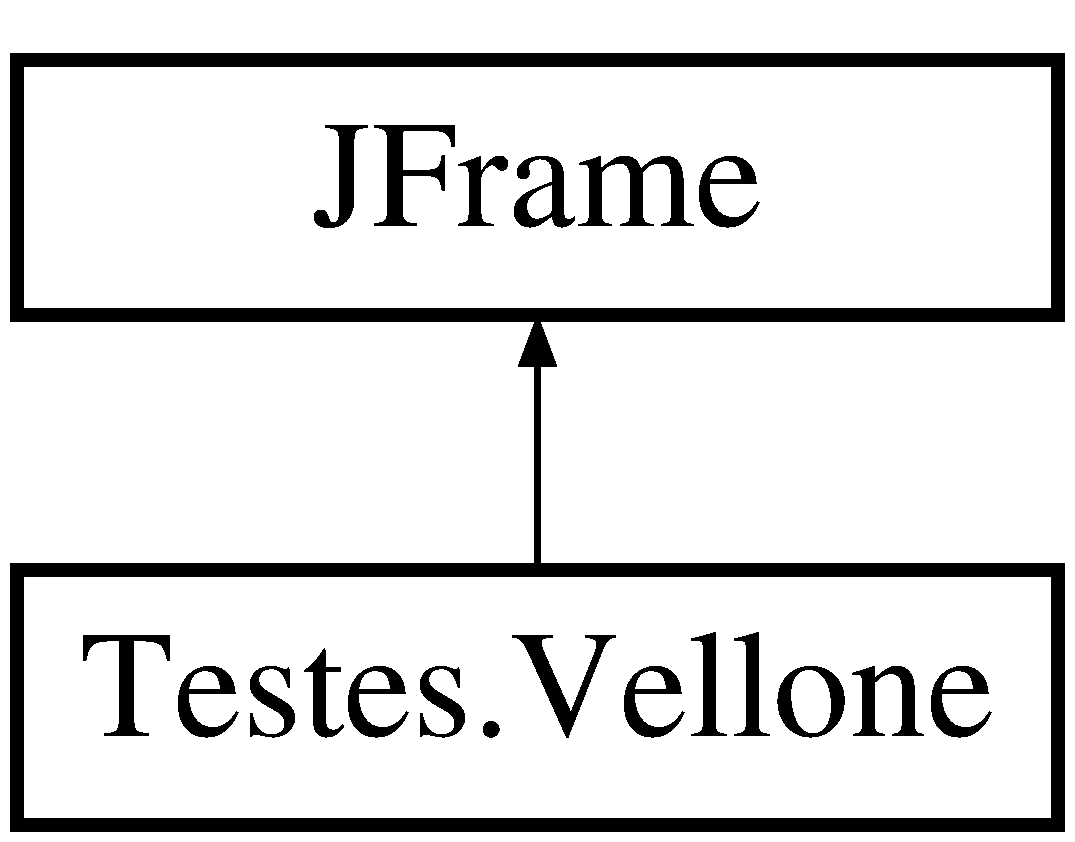
\includegraphics[height=2.000000cm]{class_testes_1_1_vellone}
\end{center}
\end{figure}
\subsection*{Static Public Member Functions}
\begin{DoxyCompactItemize}
\item 
\hypertarget{class_testes_1_1_vellone_a56452800dee4d1d21e6f25565e075201}{static void {\bfseries main} (String\mbox{[}$\,$\mbox{]} args)}\label{class_testes_1_1_vellone_a56452800dee4d1d21e6f25565e075201}

\item 
\hypertarget{class_testes_1_1_vellone_a5011c3ed8cc997410325dbf43b4f429e}{static Document {\bfseries pedir\+X\+M\+L} (String nome\+Usuario)}\label{class_testes_1_1_vellone_a5011c3ed8cc997410325dbf43b4f429e}

\end{DoxyCompactItemize}
\subsection*{Static Public Attributes}
\begin{DoxyCompactItemize}
\item 
\hypertarget{class_testes_1_1_vellone_a0cf37bfea87c820392cbfbaa30854cd3}{static \hyperlink{classservidor_1_1_sistema_arquivo}{Sistema\+Arquivo} {\bfseries teste}}\label{class_testes_1_1_vellone_a0cf37bfea87c820392cbfbaa30854cd3}

\item 
\hypertarget{class_testes_1_1_vellone_a76e1c3aef7cd74444144304ebd41bc5d}{static String {\bfseries username} = \char`\"{}vellone\char`\"{}}\label{class_testes_1_1_vellone_a76e1c3aef7cd74444144304ebd41bc5d}

\item 
\hypertarget{class_testes_1_1_vellone_a6f80c8b7ae8106d2f3ca5c042e55d141}{static \hyperlink{classjtree_1_1_x_m_l_tree_panel}{X\+M\+L\+Tree\+Panel} {\bfseries panel}}\label{class_testes_1_1_vellone_a6f80c8b7ae8106d2f3ca5c042e55d141}

\end{DoxyCompactItemize}


\subsection{Detailed Description}
\begin{DoxyAuthor}{Author}
Matheus 
\end{DoxyAuthor}


The documentation for this class was generated from the following file\+:\begin{DoxyCompactItemize}
\item 
src/\+Testes/Vellone.\+java\end{DoxyCompactItemize}

\hypertarget{classjtree_1_1_x_m_l_info_panel}{\section{jtree.\+X\+M\+L\+Info\+Panel Class Reference}
\label{classjtree_1_1_x_m_l_info_panel}\index{jtree.\+X\+M\+L\+Info\+Panel@{jtree.\+X\+M\+L\+Info\+Panel}}
}
Inheritance diagram for jtree.\+X\+M\+L\+Info\+Panel\+:\begin{figure}[H]
\begin{center}
\leavevmode
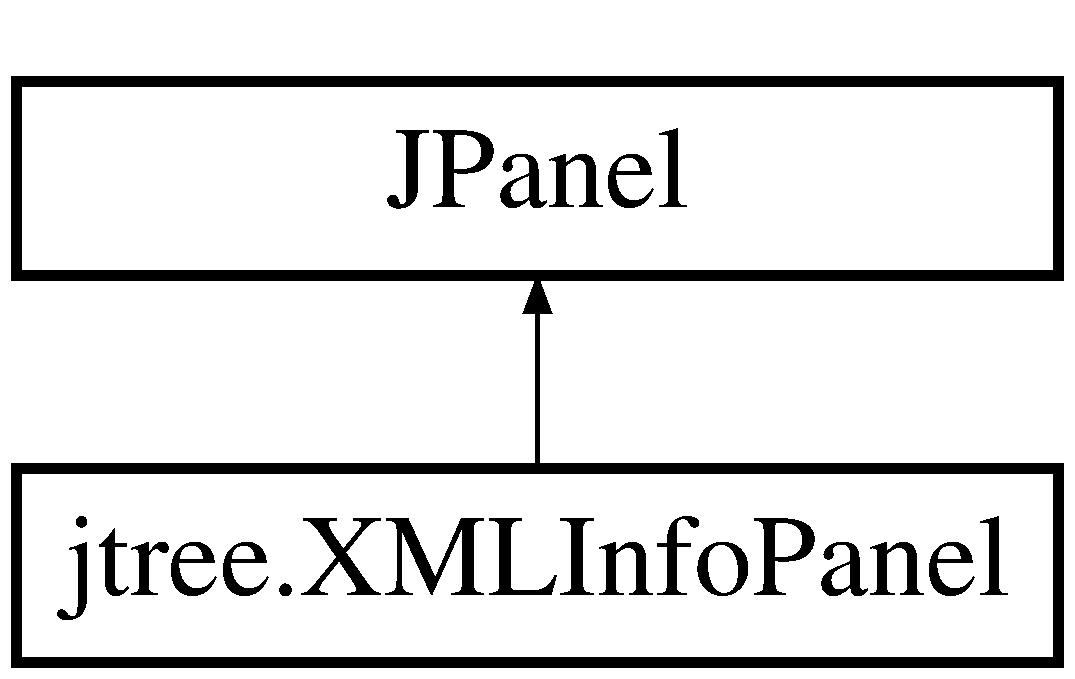
\includegraphics[height=2.000000cm]{classjtree_1_1_x_m_l_info_panel}
\end{center}
\end{figure}
\subsection*{Static Public Member Functions}
\begin{DoxyCompactItemize}
\item 
\hypertarget{classjtree_1_1_x_m_l_info_panel_aa6c86f94d049f3fe3e4a5cc45c22a257}{static void {\bfseries altera\+Info} (\hyperlink{classjtree_1_1_x_m_l_tree_node}{X\+M\+L\+Tree\+Node} node)}\label{classjtree_1_1_x_m_l_info_panel_aa6c86f94d049f3fe3e4a5cc45c22a257}

\end{DoxyCompactItemize}


The documentation for this class was generated from the following file\+:\begin{DoxyCompactItemize}
\item 
src/jtree/X\+M\+L\+Info\+Panel.\+java\end{DoxyCompactItemize}

\hypertarget{classjtree_1_1_x_m_l_menu}{\section{jtree.\+X\+M\+L\+Menu Class Reference}
\label{classjtree_1_1_x_m_l_menu}\index{jtree.\+X\+M\+L\+Menu@{jtree.\+X\+M\+L\+Menu}}
}
Inheritance diagram for jtree.\+X\+M\+L\+Menu\+:\begin{figure}[H]
\begin{center}
\leavevmode
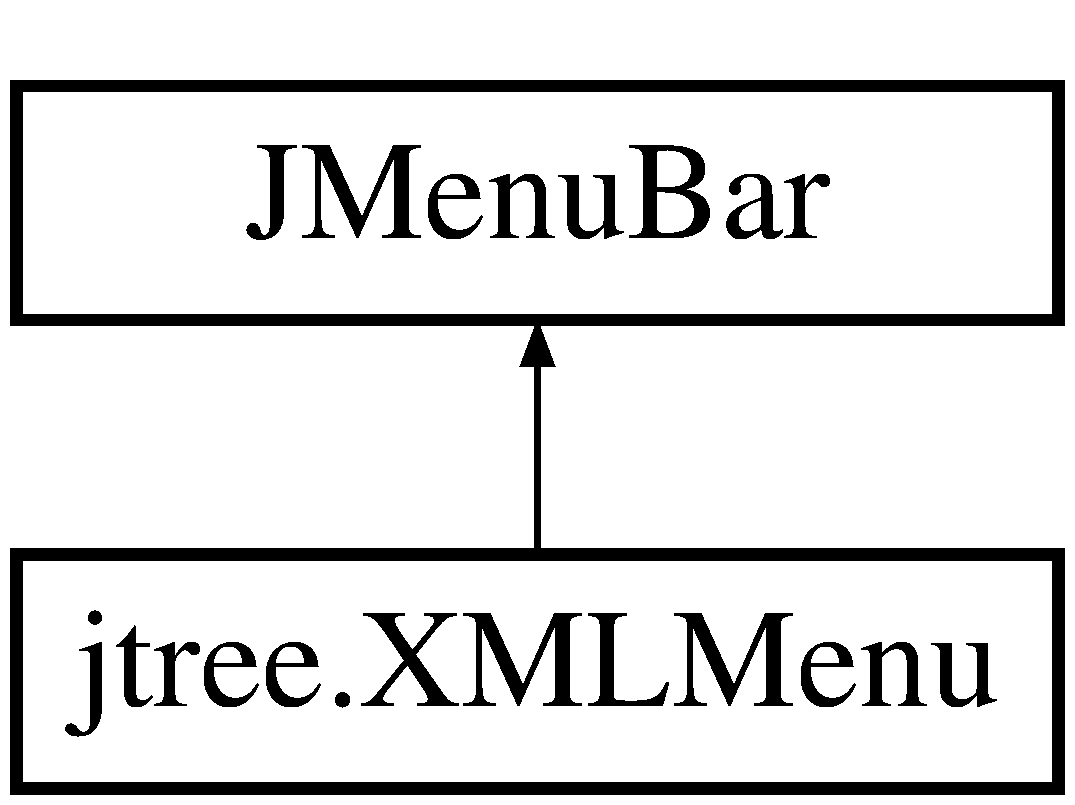
\includegraphics[height=2.000000cm]{classjtree_1_1_x_m_l_menu}
\end{center}
\end{figure}


\subsection{Detailed Description}
\begin{DoxyAuthor}{Author}
Matheus 
\end{DoxyAuthor}


The documentation for this class was generated from the following file\+:\begin{DoxyCompactItemize}
\item 
src/jtree/X\+M\+L\+Menu.\+java\end{DoxyCompactItemize}

\hypertarget{classjtree_1_1_x_m_l_tree_model}{\section{jtree.\+X\+M\+L\+Tree\+Model Class Reference}
\label{classjtree_1_1_x_m_l_tree_model}\index{jtree.\+X\+M\+L\+Tree\+Model@{jtree.\+X\+M\+L\+Tree\+Model}}
}
Inheritance diagram for jtree.\+X\+M\+L\+Tree\+Model\+:\begin{figure}[H]
\begin{center}
\leavevmode
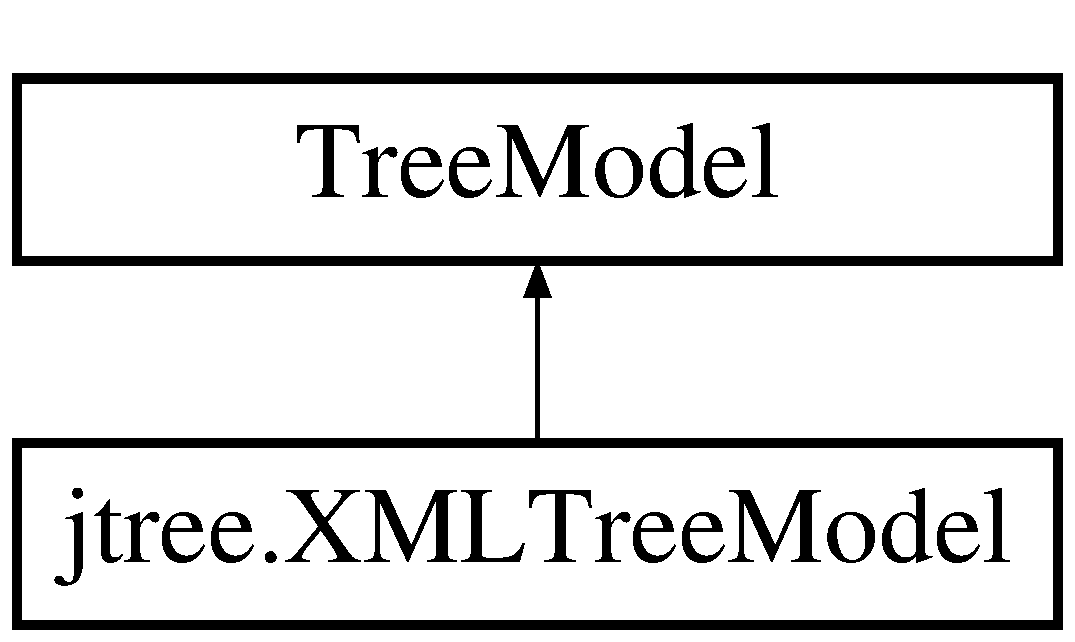
\includegraphics[height=2.000000cm]{classjtree_1_1_x_m_l_tree_model}
\end{center}
\end{figure}
\subsection*{Public Member Functions}
\begin{DoxyCompactItemize}
\item 
\hypertarget{classjtree_1_1_x_m_l_tree_model_a8dee354e383082229278c2141dfded53}{Document {\bfseries get\+Document} ()}\label{classjtree_1_1_x_m_l_tree_model_a8dee354e383082229278c2141dfded53}

\item 
\hypertarget{classjtree_1_1_x_m_l_tree_model_adcae1a6b8e5e922e0f99909c209659c3}{void {\bfseries set\+Document} (Document document)}\label{classjtree_1_1_x_m_l_tree_model_adcae1a6b8e5e922e0f99909c209659c3}

\item 
\hypertarget{classjtree_1_1_x_m_l_tree_model_a33f7d534b268f662104f387dca6edaab}{void {\bfseries add\+Tree\+Model\+Listener} (Tree\+Model\+Listener listener)}\label{classjtree_1_1_x_m_l_tree_model_a33f7d534b268f662104f387dca6edaab}

\item 
\hypertarget{classjtree_1_1_x_m_l_tree_model_af2b56c2a14f7b7e7b5975fae75331c68}{void {\bfseries remove\+Tree\+Model\+Listener} (Tree\+Model\+Listener listener)}\label{classjtree_1_1_x_m_l_tree_model_af2b56c2a14f7b7e7b5975fae75331c68}

\item 
\hypertarget{classjtree_1_1_x_m_l_tree_model_afc6f7bf08e56ddf71b42e64d628f2550}{Object {\bfseries get\+Child} (Object parent, int index)}\label{classjtree_1_1_x_m_l_tree_model_afc6f7bf08e56ddf71b42e64d628f2550}

\item 
\hypertarget{classjtree_1_1_x_m_l_tree_model_a99f4b31d62c1680aaf5d192292f36c40}{int {\bfseries get\+Child\+Count} (Object parent)}\label{classjtree_1_1_x_m_l_tree_model_a99f4b31d62c1680aaf5d192292f36c40}

\item 
\hypertarget{classjtree_1_1_x_m_l_tree_model_a2f17f6ab3e60f455eb26dbf946509224}{int {\bfseries get\+Index\+Of\+Child} (Object parent, Object child)}\label{classjtree_1_1_x_m_l_tree_model_a2f17f6ab3e60f455eb26dbf946509224}

\item 
\hypertarget{classjtree_1_1_x_m_l_tree_model_a8a52ad6dc77d41ebc615968bf8318fd9}{Object {\bfseries get\+Root} ()}\label{classjtree_1_1_x_m_l_tree_model_a8a52ad6dc77d41ebc615968bf8318fd9}

\item 
\hypertarget{classjtree_1_1_x_m_l_tree_model_ae23daf4264ddddc31a92f77962a233df}{boolean {\bfseries is\+Leaf} (Object node)}\label{classjtree_1_1_x_m_l_tree_model_ae23daf4264ddddc31a92f77962a233df}

\item 
\hypertarget{classjtree_1_1_x_m_l_tree_model_ad111c833197734e1f3cbc98258c4f54d}{void {\bfseries value\+For\+Path\+Changed} (Tree\+Path path, Object new\+Value)}\label{classjtree_1_1_x_m_l_tree_model_ad111c833197734e1f3cbc98258c4f54d}

\end{DoxyCompactItemize}


The documentation for this class was generated from the following file\+:\begin{DoxyCompactItemize}
\item 
src/jtree/X\+M\+L\+Tree\+Model.\+java\end{DoxyCompactItemize}

\hypertarget{classjtree_1_1_x_m_l_tree_node}{\section{jtree.\+X\+M\+L\+Tree\+Node Class Reference}
\label{classjtree_1_1_x_m_l_tree_node}\index{jtree.\+X\+M\+L\+Tree\+Node@{jtree.\+X\+M\+L\+Tree\+Node}}
}
\subsection*{Public Member Functions}
\begin{DoxyCompactItemize}
\item 
\hypertarget{classjtree_1_1_x_m_l_tree_node_a2b33670ebc8aedbb46d186b7a74bc9b8}{{\bfseries X\+M\+L\+Tree\+Node} (Element element)}\label{classjtree_1_1_x_m_l_tree_node_a2b33670ebc8aedbb46d186b7a74bc9b8}

\item 
\hypertarget{classjtree_1_1_x_m_l_tree_node_acfff4a1bb9c0f890ab4e7044e6940623}{Element {\bfseries get\+Element} ()}\label{classjtree_1_1_x_m_l_tree_node_acfff4a1bb9c0f890ab4e7044e6940623}

\item 
String \hyperlink{classjtree_1_1_x_m_l_tree_node_ab104ef7b456e65561ca57ba746af991e}{to\+String} ()
\item 
\hypertarget{classjtree_1_1_x_m_l_tree_node_ac71616cf5b64e75ab602f10ad2dd548a}{String {\bfseries get\+Node\+Name} ()}\label{classjtree_1_1_x_m_l_tree_node_ac71616cf5b64e75ab602f10ad2dd548a}

\end{DoxyCompactItemize}


\subsection{Member Function Documentation}
\hypertarget{classjtree_1_1_x_m_l_tree_node_ab104ef7b456e65561ca57ba746af991e}{\index{jtree\+::\+X\+M\+L\+Tree\+Node@{jtree\+::\+X\+M\+L\+Tree\+Node}!to\+String@{to\+String}}
\index{to\+String@{to\+String}!jtree\+::\+X\+M\+L\+Tree\+Node@{jtree\+::\+X\+M\+L\+Tree\+Node}}
\subsubsection[{to\+String}]{\setlength{\rightskip}{0pt plus 5cm}String jtree.\+X\+M\+L\+Tree\+Node.\+to\+String (
\begin{DoxyParamCaption}
{}
\end{DoxyParamCaption}
)}}\label{classjtree_1_1_x_m_l_tree_node_ab104ef7b456e65561ca57ba746af991e}
Retorna o valor do nó

\begin{DoxyReturn}{Returns}
String 
\end{DoxyReturn}


The documentation for this class was generated from the following file\+:\begin{DoxyCompactItemize}
\item 
src/jtree/X\+M\+L\+Tree\+Node.\+java\end{DoxyCompactItemize}

\hypertarget{classjtree_1_1_x_m_l_tree_panel}{\section{jtree.\+X\+M\+L\+Tree\+Panel Class Reference}
\label{classjtree_1_1_x_m_l_tree_panel}\index{jtree.\+X\+M\+L\+Tree\+Panel@{jtree.\+X\+M\+L\+Tree\+Panel}}
}
Inheritance diagram for jtree.\+X\+M\+L\+Tree\+Panel\+:\begin{figure}[H]
\begin{center}
\leavevmode
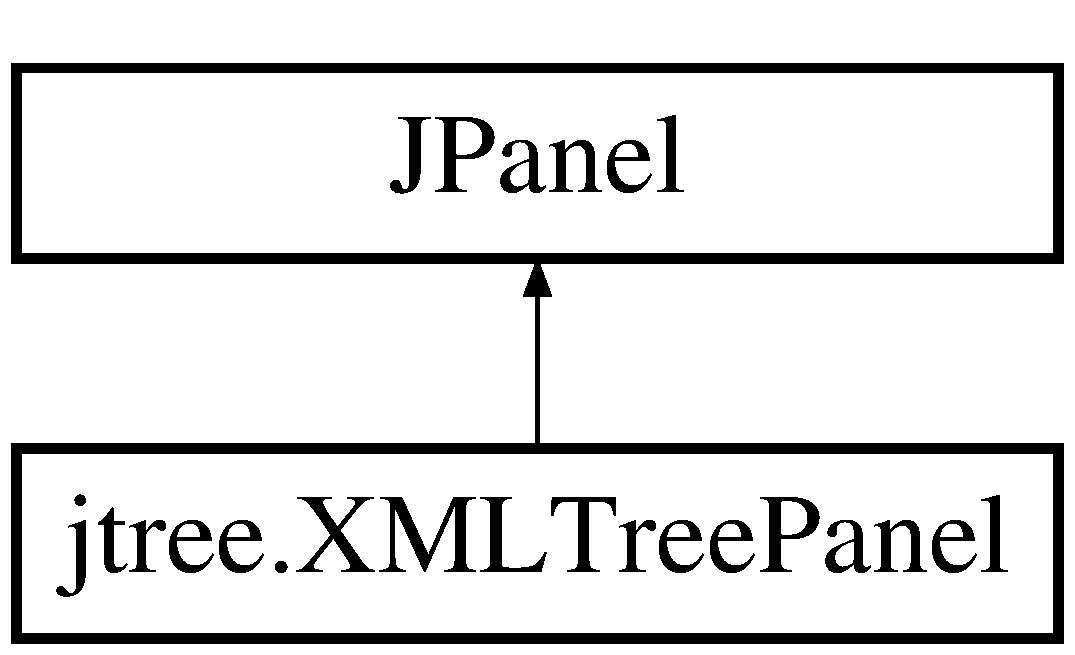
\includegraphics[height=2.000000cm]{classjtree_1_1_x_m_l_tree_panel}
\end{center}
\end{figure}
\subsection*{Public Member Functions}
\begin{DoxyCompactItemize}
\item 
\hypertarget{classjtree_1_1_x_m_l_tree_panel_a5f8ecd1ae6e234f8390d1c721874f316}{void {\bfseries set\+Document} (Document document)}\label{classjtree_1_1_x_m_l_tree_panel_a5f8ecd1ae6e234f8390d1c721874f316}

\item 
\hypertarget{classjtree_1_1_x_m_l_tree_panel_ade28954653ce35c35f40600e0b3e93ba}{Document {\bfseries get\+Document} ()}\label{classjtree_1_1_x_m_l_tree_panel_ade28954653ce35c35f40600e0b3e93ba}

\end{DoxyCompactItemize}
\subsection*{Static Public Member Functions}
\begin{DoxyCompactItemize}
\item 
static String \hyperlink{classjtree_1_1_x_m_l_tree_panel_a81425c3872cdd53e2fd22fbf62525d27}{get\+Caminho\+Selecionado} (boolean excluir\+Ultimo)
\item 
static void \hyperlink{classjtree_1_1_x_m_l_tree_panel_af2187a25fe036fb8fee80bce7827747a}{atualiza\+Arvore} ()
\end{DoxyCompactItemize}
\subsection*{Static Public Attributes}
\begin{DoxyCompactItemize}
\item 
\hypertarget{classjtree_1_1_x_m_l_tree_panel_a63e930f23823e91bb342d49739a68a97}{static J\+Tree {\bfseries tree}}\label{classjtree_1_1_x_m_l_tree_panel_a63e930f23823e91bb342d49739a68a97}

\item 
\hypertarget{classjtree_1_1_x_m_l_tree_panel_af72534f1f5ade0a487c7ef7c886ed737}{static \hyperlink{classjtree_1_1_x_m_l_tree_node}{X\+M\+L\+Tree\+Node} {\bfseries node\+\_\+selecionado}}\label{classjtree_1_1_x_m_l_tree_panel_af72534f1f5ade0a487c7ef7c886ed737}

\end{DoxyCompactItemize}


\subsection{Member Function Documentation}
\hypertarget{classjtree_1_1_x_m_l_tree_panel_af2187a25fe036fb8fee80bce7827747a}{\index{jtree\+::\+X\+M\+L\+Tree\+Panel@{jtree\+::\+X\+M\+L\+Tree\+Panel}!atualiza\+Arvore@{atualiza\+Arvore}}
\index{atualiza\+Arvore@{atualiza\+Arvore}!jtree\+::\+X\+M\+L\+Tree\+Panel@{jtree\+::\+X\+M\+L\+Tree\+Panel}}
\subsubsection[{atualiza\+Arvore}]{\setlength{\rightskip}{0pt plus 5cm}static void jtree.\+X\+M\+L\+Tree\+Panel.\+atualiza\+Arvore (
\begin{DoxyParamCaption}
{}
\end{DoxyParamCaption}
)\hspace{0.3cm}{\ttfamily [static]}}}\label{classjtree_1_1_x_m_l_tree_panel_af2187a25fe036fb8fee80bce7827747a}
Função para atualizar a árvore de hierarquia após modificar o X\+M\+L \hypertarget{classjtree_1_1_x_m_l_tree_panel_a81425c3872cdd53e2fd22fbf62525d27}{\index{jtree\+::\+X\+M\+L\+Tree\+Panel@{jtree\+::\+X\+M\+L\+Tree\+Panel}!get\+Caminho\+Selecionado@{get\+Caminho\+Selecionado}}
\index{get\+Caminho\+Selecionado@{get\+Caminho\+Selecionado}!jtree\+::\+X\+M\+L\+Tree\+Panel@{jtree\+::\+X\+M\+L\+Tree\+Panel}}
\subsubsection[{get\+Caminho\+Selecionado}]{\setlength{\rightskip}{0pt plus 5cm}static String jtree.\+X\+M\+L\+Tree\+Panel.\+get\+Caminho\+Selecionado (
\begin{DoxyParamCaption}
\item[{boolean}]{excluir\+Ultimo}
\end{DoxyParamCaption}
)\hspace{0.3cm}{\ttfamily [static]}}}\label{classjtree_1_1_x_m_l_tree_panel_a81425c3872cdd53e2fd22fbf62525d27}
Monta uma String com o caminho do item selecionado. Se o item selecionado é um arquivo e o parametro é true, o último elemento é excluido do caminho


\begin{DoxyParams}{Parameters}
{\em excluir\+Ultimo} & boolean -\/ true\+: excluir o último item do caminho, caso este seja um arquivo; false\+: não tira o último elemento, seja um arquivo ou não \\
\hline
\end{DoxyParams}
\begin{DoxyReturn}{Returns}
String -\/ caminho do item selecionado na árvore de hierarquia 
\end{DoxyReturn}


The documentation for this class was generated from the following file\+:\begin{DoxyCompactItemize}
\item 
src/jtree/X\+M\+L\+Tree\+Panel.\+java\end{DoxyCompactItemize}

%--- End generated contents ---

% Index
\newpage
\phantomsection
\addcontentsline{toc}{chapter}{Index}
\printindex

\end{document}
